% presentation

%\documentclass{beamer}
%\usetheme[height=7mm]{Rochester}
%\usecolortheme{rose}

% handout

\documentclass[handout]{beamer}
\usepackage{pgfpages} \pgfpagesuselayout{16 on 1}[a4paper,landscape]

%\documentclass[mathserif]{article}
%\usepackage{beamerarticle}

\usepackage{amsmath}
\usepackage{amssymb,amsfonts}
\usepackage[T1]{fontenc}
\usepackage{lmodern}
\usepackage{tikz}
\usepackage{comment}
\usepackage{simpsons}
\usepackage{marvosym}
\usepackage{color}
\usepackage{multirow}
\usepackage{pgffor}
\usepackage{pgfplots}
\usepackage[slide,algoruled,titlenumbered,vlined,noend,linesnumbered,]{algorithm2e}

% handout
%\usefonttheme{structurebold}

\setbeamertemplate{footline}[frame number]
\setbeamertemplate{navigation symbols}{}
\setbeamerfont{smallverb}{size*={73}}
\usefonttheme[onlymath]{serif}
\setbeamertemplate{theorems}[numbered]
\newtheorem{construction}[theorem]{Construction}
\newtheorem{proposition}[theorem]{Proposition}

%\AtBeginSection[] { 
%  \begin{frame} 
%    \frametitle{Content} 
%    \tableofcontents[currentsection]
%  \end{frame} 
%  \addtocounter{framenumber}{-1} 
%}

\usetikzlibrary[shapes.arrows]
\usetikzlibrary{shapes.geometric}
\usetikzlibrary{backgrounds}
\usetikzlibrary{positioning}
\usetikzlibrary{calc}
\usetikzlibrary{intersections}
\usetikzlibrary{fadings}
\usetikzlibrary{decorations.footprints}
\usetikzlibrary{patterns}
\usetikzlibrary{shapes.callouts}
\usetikzlibrary{fit}
%handout

\providecommand{\abs}[1]{\lvert#1\rvert}

%\tikzset{every picture/.style={line width=1pt,show background rectangle},background rectangle/.style={fill=blue!10,rounded corners=2ex}}

\newcommand{\Bob}[3]{ \begin{scope}[shift={(#1,#2)},scale=#3]
    \draw (0,0) circle (0.95 and 1);
    \fill (-0.3,-0.1) circle (0.1);
    \fill (+0.3,-0.1) circle (0.1);
    \draw (0.35,-0.5) arc (-70:-110: 1 and 0.4);
    \draw (-0.3,0.5) arc (-10:-80: 0.8 and 0.8);
    \draw (-0.5,0.8) arc (190:255: 2 and 1);
    \draw (-0.7,0.9) -- +(0.2,-0.09) -- +(0.25,0.2);
    \end{scope} }
  
\newcommand{\Alice}[3]{ \begin{scope}[shift={(#1,#2)},scale=#3]
  \draw (0,0) circle (0.95 and 1);
  \fill (-0.3,-0.1) circle (0.1);
  \fill (+0.3,-0.1) circle (0.1);
  \draw (0.35,-0.5) arc (-70:-110: 1 and 0.4);
  \draw (0.3,1.3) arc (20:-100: 1.4 and 1);
  \draw (0.5,1.3) arc (150:260: 1 and 1);
  \draw (0.41,1.3) circle (0.35);
  \end{scope} }

  \newcommand{\Evil}[3]{ \begin{scope}[shift={(#1,#2)},scale=#3]
    \draw (0,0) circle (0.95 and 1);
    \fill (-0.1,-0.1) -- +(-0.2,-0.1) -- +(-0.4,0.2); %eye
    \fill (0.1,-0.1) -- +(0.2,-0.1) -- +(0.4,0.2);
    \draw (0.35,-0.5) arc (-70:-110: 1 and 0.4);
    %\fill (0.3,-0.5) -- +(-0.1,-0.2) -- +(-0.2,-0.02);
    %\fill (-0.3,-0.5) -- +(0.1,-0.2) -- +(0.2,-0.02);
    \fill (0.3,0.7) -- +(0.5,0.4) -- +(0.4,-0.2); % horn
    \fill (-0.3,0.7) -- +(-0.5,0.4) -- +(-0.4,-0.2);
    %\draw (0.3,1.3) arc (20:-100: 1.4 and 1);
    %\draw (0.5,1.3) arc (150:260: 1 and 1);
    %\draw (0.41,1.3) circle (0.35);
    \end{scope} }

\newcommand{\Charlie}[3]{ \begin{scope}[shift={(#1,#2)},scale=#3]
    \draw (0,0) circle (0.95 and 1);
    \filldraw[fill=black!20] (-0.35,-0.1) circle (0.25);
    \filldraw[fill=black!20] (+0.35,-0.1) circle (0.25);
    %\draw (0.9,0.2) to [bend left] (-0.9,0.2);
    \draw (0.2,0) to [bend left] (-0.2,0);


    %\draw (0.3,0.7) to [bend right] (-0.3,0.7);
    %\draw (0.4,0.5) to [bend right] (-0.4,0.5);
    %\draw (0.35,-0.5) arc (-70:-110: 1 and 0.4);
    \draw (-0.7,-0.6) to [bend right] (0,-0.6) to [bend right] (0.7,-0.6) to [bend right]  (0,-0.5)  to [bend right]  cycle ;
    %\draw (0.3,1.3) arc (20:-100: 1.4 and 1);
    %\draw (0.5,1.3) arc (150:260: 1 and 1);
    %\draw (0.41,1.3) circle (0.35);
    \end{scope} }

\author{Yu Zhang}
\institute{HIT/CST/NIS}
\date[Crypt'12S]{Cryptography, Spring, 2012}

%% presentation
\documentclass{beamer}
\usetheme[height=7mm]{Rochester}
\usecolortheme{rose}

% handout

%\documentclass[handout]{beamer}
%\usepackage{pgfpages} \pgfpagesuselayout{8 on 1}[a4paper]

%\documentclass[mathserif]{article}
%\usepackage{beamerarticle}

\usepackage{amsmath}
\usepackage{comment}
\usepackage{amssymb,amsfonts}
\usepackage[T1]{fontenc}
\usepackage{lmodern}
\usepackage{tikz}
%\usepackage{simpsons}
\usepackage{marvosym}
\usepackage{color}
\usepackage{multirow}
\usepackage{pgffor}
\usepackage{pgfplots}
\usepackage[slide,algoruled,titlenumbered,vlined,noend,linesnumbered,]{algorithm2e}

\usefonttheme{structurebold}

\setbeamertemplate{footline}[frame number]
\setbeamertemplate{navigation symbols}{}
\setbeamerfont{smallverb}{size*={73}}
\usefonttheme[onlymath]{serif}
\setbeamertemplate{theorems}[numbered]
\newtheorem{construction}[theorem]{Construction}
\newtheorem{proposition}[theorem]{Proposition}

\AtBeginSection[] {
  \begin{frame}
    \frametitle{Content}
    \tableofcontents[currentsection]
  \end{frame}
  \addtocounter{framenumber}{-1}
}

\usetikzlibrary[shapes.arrows]
\usetikzlibrary{shapes.geometric}
\usetikzlibrary{backgrounds}
\usetikzlibrary{positioning}
\usetikzlibrary{calc}
\usetikzlibrary{intersections}
\usetikzlibrary{fadings}
\usetikzlibrary{decorations.footprints}
\usetikzlibrary{patterns}
\usetikzlibrary{shapes.callouts}
\usetikzlibrary{fit}
%handout

\providecommand{\abs}[1]{\lvert#1\rvert}

\tikzset{every picture/.style={line width=1pt,show background rectangle},background rectangle/.style={fill=blue!10,rounded corners=2ex}}

\newcommand{\Bob}[3]{ \begin{scope}[shift={(#1,#2)},scale=#3]
  \draw (0,0) circle (0.95 and 1);
  \fill (-0.3,-0.1) circle (0.1);
  \fill (+0.3,-0.1) circle (0.1);
  \draw (0.35,-0.5) arc (-70:-110: 1 and 0.4);
  \draw (-0.3,0.5) arc (-10:-80: 0.8 and 0.8);
  \draw (-0.5,0.8) arc (190:255: 2 and 1);
  \draw (-0.7,0.9) -- +(0.2,-0.09) -- +(0.25,0.2);
  \end{scope} }

\newcommand{\Alice}[3]{ \begin{scope}[shift={(#1,#2)},scale=#3]
  \draw (0,0) circle (0.95 and 1);
  \fill (-0.3,-0.1) circle (0.1);
  \fill (+0.3,-0.1) circle (0.1);
  \draw (0.35,-0.5) arc (-70:-110: 1 and 0.4);
  \draw (0.3,1.3) arc (20:-100: 1.4 and 1);
  \draw (0.5,1.3) arc (150:260: 1 and 1);
  \draw (0.41,1.3) circle (0.35);
  \end{scope} }

  \newcommand{\Evil}[3]{ \begin{scope}[shift={(#1,#2)},scale=#3]
    \draw (0,0) circle (0.95 and 1);
    \fill (-0.1,-0.1) -- +(-0.2,-0.1) -- +(-0.4,0.2); %eye
    \fill (0.1,-0.1) -- +(0.2,-0.1) -- +(0.4,0.2);
    \draw (0.35,-0.5) arc (-70:-110: 1 and 0.4);
    %\fill (0.3,-0.5) -- +(-0.1,-0.2) -- +(-0.2,-0.02);
    %\fill (-0.3,-0.5) -- +(0.1,-0.2) -- +(0.2,-0.02);
    \fill (0.3,0.7) -- +(0.5,0.4) -- +(0.4,-0.2); % horn
    \fill (-0.3,0.7) -- +(-0.5,0.4) -- +(-0.4,-0.2);
    %\draw (0.3,1.3) arc (20:-100: 1.4 and 1);
    %\draw (0.5,1.3) arc (150:260: 1 and 1);
    %\draw (0.41,1.3) circle (0.35);
    \end{scope} }

\newcommand{\Charlie}[3]{ \begin{scope}[shift={(#1,#2)},scale=#3]
    \draw (0,0) circle (0.95 and 1);
    \filldraw[fill=black!20] (-0.35,-0.1) circle (0.25);
    \filldraw[fill=black!20] (+0.35,-0.1) circle (0.25);
    %\draw (0.9,0.2) to [bend left] (-0.9,0.2);
    \draw (0.2,0) to [bend left] (-0.2,0);


    %\draw (0.3,0.7) to [bend right] (-0.3,0.7);
    %\draw (0.4,0.5) to [bend right] (-0.4,0.5);
    %\draw (0.35,-0.5) arc (-70:-110: 1 and 0.4);
    \draw (-0.7,-0.6) to [bend right] (0,-0.6) to [bend right] (0.7,-0.6) to [bend right]  (0,-0.5)  to [bend right]  cycle ;
    %\draw (0.3,1.3) arc (20:-100: 1.4 and 1);
    %\draw (0.5,1.3) arc (150:260: 1 and 1);
    %\draw (0.41,1.3) circle (0.35);
    \end{scope} }

\author{Yu Zhang}
\institute{Harbin Institute of Technology}
\date[Crypto'22A]{Cryptography, Autumn, 2022}

%\input{1introduction.tex}
%\input{2perfectlysecret.tex}
%\input{3privatekey.tex}


\title{Introduction}

\begin{document}
\maketitle
\begin{frame}
\frametitle{Outline}
\tableofcontents
\end{frame}
\section{Cryptography and Modern Cryptography}
\begin{frame}\frametitle{What is Cryptography?}
\begin{itemize}
\item \textbf{Cryptography}: from Greek \emph{krypt\'os}, ``hidden, secret''; and \emph{gr\'{a}phin}, ``writing''
\item \textbf{Cryptography}: the art of writing or solving codes.\\ (Concise oxford dictionary 2006)
\item \textbf{Codes}: a system of prearranged signals, especially used to ensure secrecy in transmitting messages. \\ (\emph{code word} in cryptography)
\item \textbf{1980s}: from Classic to Modern; from Military to Everyone
\item \textbf{Modern cryptography}: the scientific study of mathematical techniques for securing digital information, systems, and distributed computations against adversarial attacks
\end{itemize}
\end{frame}
\begin{frame}\frametitle{What is cryptography? [xkcd:504]}
\begin{figure}
\begin{center}
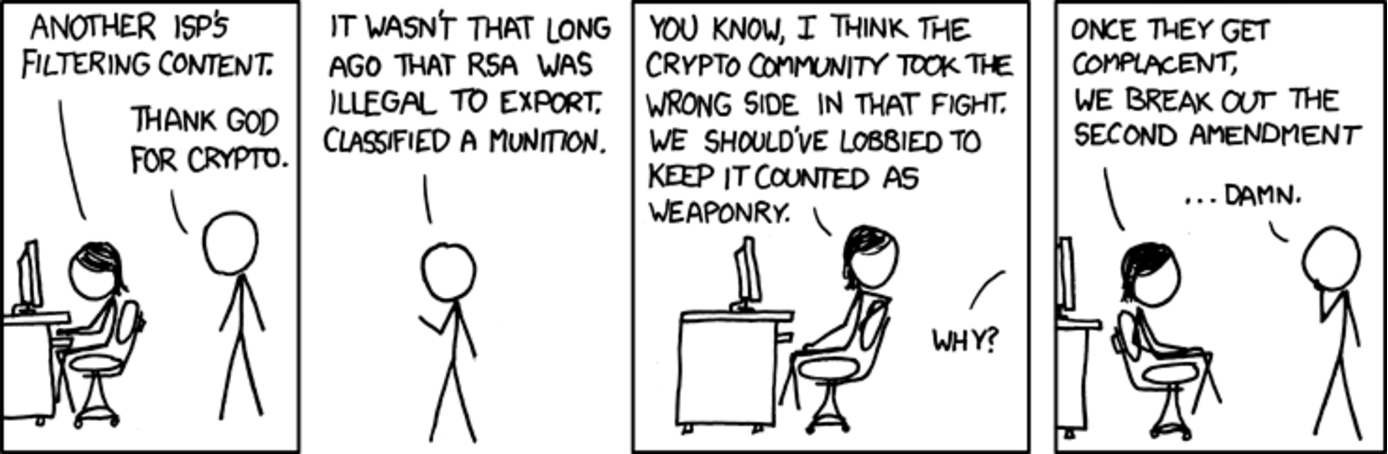
\includegraphics[width=100mm]{pic/legal} 
\end{center}
\end{figure}
\end{frame}
\section{The Setting of Private-Key Encryption}
\begin{frame}\frametitle{Private-Key Encryption}
\begin{itemize}
\item \textbf{Goal}: to construct \textbf{ciphers} (encryption schemes) for providing secret communication between two parties sharing \textbf{private-key} (the symmetric-key) in advance
\item \textbf{Implicit assumption}: there is some way of initially sharing a key in a secret manner
\item \textbf{Disk encryption}: the same user at different points in time
\end{itemize}
\end{frame}
\begin{frame}\frametitle{Alice, Bob  [xkcd:1323]}
Changing the names would be easier, but if you're not comfortable lying, try only making friends with people named Alice, Bob, Carol, etc.
\begin{figure}
\begin{center}
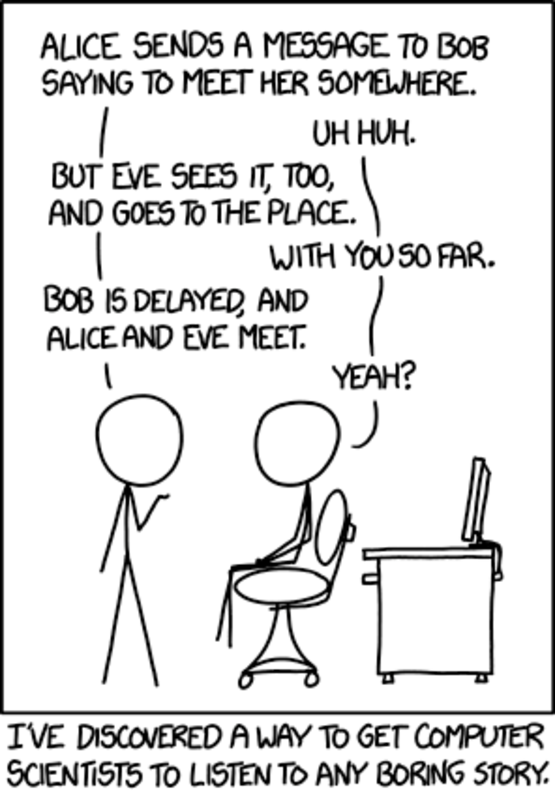
\includegraphics[width=45mm]{pic/alice-bob} 
\end{center}
\end{figure}
\end{frame}
\begin{frame}\frametitle{The Syntax of Encryption}
\begin{figure}
\begin{center}
\begin{tikzpicture}
\node (sender) [minimum size=1cm] {}; \Alice{0}{0}{0.4};
\node (bart) [below of = sender, node distance = 0.7cm] {Alice};
\node (enc) [draw, right of = sender, rounded corners=1ex,node distance = 2cm] {$\mathsf{Enc}$};
\node (k1) [above of = enc, node distance = 1cm] {$k$};
\node (c) [right of = enc, node distance = 2cm] {$c$};
\node (gen) [draw, above of = c, rounded corners=1ex,node distance = 1cm] {$\mathsf{Gen}$};
\node (adv) [below of = c, node distance = 1cm, minimum size=1cm] {}; \Evil{4cm}{-1cm}{0.4};
\node (burns) [below of = adv, node distance = 0.7cm] {Adversary};
\node (dec) [draw, right of = c, rounded corners=1ex,node distance = 2cm] {$\mathsf{Dec}$};
\node (k2) [above of = dec, node distance = 1cm] {$k$};
\node (receiver) [right of = dec, node distance = 2cm, minimum size=1cm] {}; \Bob{8cm}{0}{0.4};
\node (lisa) [below of = receiver, node distance = 0.7cm] {Bob};
\draw[-latex] (sender) -- (enc) node [midway, above] {$m$};
\draw (enc) -- (c); \draw[-latex] (c) -- (dec);
\draw[-latex] (dec) -- (receiver) node [midway, above] {$m$};
\draw[-latex] (k1) -- (enc);
\draw[-latex] (gen) -- (k1);
\draw[-latex] (gen) -- (k2);								
\draw[-latex] (k2) -- (dec);		
\end{tikzpicture}
\end{center}
\end{figure}
\begin{itemize}
\item key $k \in \mathcal{K}$, plaintext (or message) $m \in \mathcal{M}$, ciphertext $c \in \mathcal{C}$
\item \textbf{Key-generation} algorithm~$k \gets \mathsf{Gen}$
\item \textbf{Encryption} algorithm~$c:= \mathsf{Enc}_k(m)$
\item \textbf{Decryption} algorithm~$m:= \mathsf{Dec}_k(c)$
\item \textbf{Encryption scheme}: $\Pi = (\mathsf{Gen}, \mathsf{Enc}, \mathsf{Dec})$
\item \textbf{Basic correctness requirement}: $\mathsf{Dec}_k(\mathsf{Enc}_k(m)) = m$
\end{itemize}
\end{frame}
\begin{frame}\frametitle{Securing Key vs Obscuring Algorithm}
\begin{itemize}
\item Easier to maintain secrecy of a short key
\item In case the key is exposed, easier for the honest parties to change the key
\item In case many pairs of people, easier to use the same algorithm, but different keys
\end{itemize}
\begin{alertblock}{Kerckhoffs's principle}
\begin{quote}
The cipher method must not be required to be secret, and it must be able to fall into the hands of the enemy without inconvenience.
\end{quote}	
\end{alertblock}
\begin{alertblock}{Shannon's maxim}
	\begin{quote}
		The enemy knows the system.
	\end{quote}	
\end{alertblock}
\end{frame}
\begin{frame}\frametitle{Why ``Open Cryptographic Design''}
\begin{itemize}
\item Published designs undergo public scrutiny are to be stronger
\item Better for security flaws to be revealed by ``ethical hackers''
\item Reverse engineering of the code (or leakage by industrial espionage) poses a serious threat to security
\item Enable the establishment of standards.
\end{itemize}
\begin{exampleblock}{Dual EC: A Standardized Back Door}
	``Dual EC was standardized by NIST, ANSI, and ISO among other algorithms to generate pseudorandom numbers.'' ``The Snowden revelations, and in particular reports on Project Bullrun and the SIGINT Enabling Project, have indicated that Dual EC was part of a systematic effort by NSA to subvert standards.'' ``Reuters reported that NSA paid RSA ``\$10 million in a deal that set [Dual EC] as the preferred, or default, method for number generation in the BSafe software.''''	
\end{exampleblock}
\end{frame}
\begin{frame}\frametitle{Attack Scenarios}	
\begin{itemize}
\item \textbf{Ciphertext-only}: the adversary just observes ciphertext
\item \textbf{Known-plaintext}: the adversary learns pairs of plaintexts/ciphertexts under the same key
\item \textbf{Chosen-plaintext}: the adversary has the ability to obtain the encryption of plaintexts of its choice
\item \textbf{Chosen-ciphertext}: the adversary has the ability to obtain the decryption of \textbf{other} ciphertexts of its choice
\item \textbf{Passive attack}: COA KPA
\begin{itemize}
\item because not all ciphertext are confidential
\end{itemize}
\item \textbf{Active attack}: CPA CCA
\begin{itemize}
\item when to encrypt/decrypt whatever an adversary wishes?
\end{itemize}
\end{itemize}	
\end{frame}
\section{Historical Ciphers and Their Cryptanalysis}
\begin{comment}
	\begin{frame}\frametitle{Why We Learn Broken Ciphers?}
	\begin{itemize}
	\item To understand the weaknesses of an ``ad-hoc'' approach
	\item To learn that ``simple'' approaches are unlikely to succeed
	\item To feel that ``we are smart enough to do some crypt-analyzing''
	\end{itemize}
	\end{frame}
\end{comment}

\begin{frame}[fragile]\frametitle{Caesar's Cipher}
\begin{quote}
If he had anything confidential to say, he wrote it in cipher, that is, by so changing the order of the letters of the alphabet, that not a word could be made out. If anyone wishes to \alert{decipher} these, and get at their meaning, he must \alert{substitute the fourth letter of the alphabet, namely D, for A}, and so with the others

\rightline{--Suetonius,``Life of Julius Caesar''}
\end{quote}
\begin{itemize}
	\item $\mathsf{Enc}(m)=m+3\mod 26$ \footnote{In fact the quote indicates that decryption involved rotating letters of the alphabet forward 3 positions, $\mathsf{Dec}(c)=c+3\mod 26$}
	\item \textbf{Weakness}: ? %\alert{What is the key?}
\end{itemize}
\begin{exampleblock}{Example}
\verb|begintheattacknow|
%\verb|EHJLQWKHDWWDFNQRZ|
\end{exampleblock}
\end{frame}
\begin{frame}[fragile]\frametitle{Shift Cipher}
\begin{itemize}
\item $\mathsf{Enc}_k(m)=m+k\mod 26$
\item $\mathsf{Dec}_k(c)=c-k\mod 26$
\item \textbf{Weakness}: ? %Fragile under \textbf{Brute-force attack} (exhaustive search)
\end{itemize}
\begin{exampleblock}{Example: Decipher the string}	
\verb|EHJLQWKHDWWDFNQRZ|
\end{exampleblock}
\begin{alertblock}{Sufficient Key Space Principle}
Any secure encryption scheme must have a key space that is not vulnerable to exhaustive search.\footnote{If the plaintext space is larger than the key space.}
\end{alertblock}
\end{frame}
\begin{frame}\frametitle{Index of Coincidence (IC) Method (to find $k$)}
\textbf{How to automatically determine that the deciphered text makes sense?}

\textbf{Index of Coincidence (IC)}: the probability that two randomly selected letters (pick-then-return) will be identical.

Let $p_i$ denote the probability of $i$th letter in English text.
\[I \overset{\text{def}}{=}\sum_{i=0}^{25} p_i^2 \]
\begin{exampleblock}{Example}
What's the IC of `apple'?
\end{exampleblock}

For a long English text, the IC is $\approx 0.065$.
For $j = 0, 1, \dotsc , 25$, $q_j$ is the probability of $j$th letter in the ciphertext.
\[I_j \overset{\text{def}}{=}\sum_{i=0}^{25} p_i \cdot q_{i+j}\]
\alert{Q: For shift cipher, if $j = k$, then $I_j \approx$ ?}
\end{frame}

\begin{frame}[fragile]\frametitle{Mono-Alphabetic Substitution}
\begin{itemize}
\item \textbf{Idea}: To map each character to a different one in an arbitrary manner
\item \textbf{Strength}: Key space is large $\approx 2^{88}$. \alert{Q: how to count?}
\item \textbf{Weakness}: ? %The mapping of each letter is fixed
\end{itemize}
\begin{exampleblock}{Example}
\verb|abcdefghijklmnopqrstuvwxyz|\\
\verb|XEUADNBKVMROCQFSYHWGLZIJPT|

Plaintext: \verb|tellhimaboutme|\\
Ciphertext: \verb|??????????????|
\end{exampleblock}
\end{frame}
\begin{frame}[fragile]\frametitle{Attack with Statistical Patterns}
\begin{enumerate}
\item Tabulate the frequency of letters in the ciphertext
\item Compare it to those in English text
\item Guess the most frequent letter corresponds to \verb|e|, and so on
\item Choose the plaintext that does ``make sense'' (Not trivial)
\end{enumerate}
\begin{table}
\begin{center}
\caption{Average letter frequencies for English-language text}
\begin{tabular}{|cc|cc|cc|cc|cc|} \hline
e & 12.7\% & t & 9.1\% & a & 8.2\% & o & 7.5\% & i & 7.0\%\\
n & 6.7\% & \_ & 6.4\% & s & 6.3\% & h & 6.1\% & r & 6.0\%\\
d & 4.3\% & l & 4.0\% & c & 2.8\% & u & 2.8\% & m & 2.4\%\\
w & 2.4\% & f & 2.2\% & g & 2.0\% & y & 2.0\% & p & 1.9\%\\
b & 1.5\% & v & 1.0\% & k & 0.8\% & j & 0.2\% & x & 0.2\%\\
q & 0.1\% & z & 0.1\% & & & & & &\\ \hline
\end{tabular}
\end{center}
\end{table}
\end{frame}
\begin{frame}[fragile]\frametitle{Example of Frequency Analysis (Ciphertext)}
\begin{verbatim}
LIVITCSWPIYVEWHEVSRIQMXLEYVEOIEWHRXEXIPFEMVEWHKVS
TYLXZIXLIKIIXPIJVSZEYPERRGERIMWQLMGLMXQERIWGPSRIH
MXQEREKIETXMJTPRGEVEKEITREWHEXXLEXXMZITWAWSQWXSWE
XTVEPMRXRSJGSTVRIEYVIEXCVMUIMWERGMIWXMJMGCSMWXSJO
MIQXLIVIQIVIXQSVSTWHKPEGARCSXRWIEVSWIIBXVIZMXFSJX
LIKEGAEWHEPSWYSWIWIEVXLISXLIVXLIRGEPIRQIVIIBGIIHM
WYPFLEVHEWHYPSRRFQMXLEPPXLIECCIEVEWGISJKTVWMRLIHY
SPHXLIQIMYLXSJXLIMWRIGXQEROIVFVIZEVAEKPIEWHXEAMWY
EPPXLMWYRMWXSGSWRMHIVEXMSWMGSTPHLEVHPFKPEZINTCMXI
VJSVLMRSCMWMSWVIRCIGXMWYMX
\end{verbatim}
\end{frame}
\begin{frame}[fragile]\frametitle{Example of Frequency Analysis (Analysis)}
Count and Guess, Trial and Error.
\begin{table}
\begin{center}
\caption{Analysis Steps}
\begin{tabular}{|r|l|} \hline
Ciphertext & Plaintext \\ \hline
\alert{I}   & \alert{e} \\
\alert{XLI} & \alert{the} \\
\alert{E} & \alert{a} \\
\alert{R}tate & \alert{s}tate \\
atthatt\alert{MZ}e & atthatt\alert{im}e \\
he\alert{V}e & he\alert{r}e \\
remar\alert{A} & remar\alert{k} \\ \hline
\end{tabular}
\end{center}
\end{table}
\end{frame}
\begin{frame}[fragile]\frametitle{Example of Frequency Analysis (Plaintext)}
\begin{quote}
Hereupon Legrand arose, with a grave and stately air, and brought me the beetle
from a glass case in which it was enclosed. It was a beautiful scarabaeus, and, at
that time, unknown to naturalists -- of course a great prize in a scientific point
of view. There were two round black spots near one extremity of the back, and a
long one near the other. The scales were exceedingly hard and glossy, with all the
appearance of burnished gold. The weight of the insect was very remarkable, and,
taking all things into consideration, I could hardly blame Jupiter for his opinion
respecting it.

\rightline{--Edgar Allan Poe's ``The Gold-Bug''}
\end{quote}
\end{frame}

\begin{frame}[fragile]\frametitle{Vigen\`{e}re (poly-alphabetic shift) Cipher}
\begin{itemize}
\item \textbf{Idea}: To ``smooth out'' the distribution in the ciphertext by mapping different instances of the same letter in the plaintext to different ones in the ciphertext
\item \textbf{Encryption}: $c_i=m_i+k_{[i\bmod t]}$, $t$ is the length (period) of $k$
\item \textbf{Cryptanalysis}: Need find $t$; if $t$ is known, need know whether the decryption ``makes sense'', but brute force ($26^t$) is infeasible for $t > 15$
\end{itemize}
\begin{exampleblock}{Example (Key is `cafe')}
\begin{description}[Ciphertext]
\item[Plaintext]  \verb|tellhimaboutme| \\
\item[Key]        \verb|cafecafecafeca| \\
\item[Ciphertext] \verb|??????????????| %\verb|WFRQKJSFEPAYPF|
\end{description}
\end{exampleblock}
\end{frame}
\begin{frame}[fragile]\frametitle{Kasiski's Method (to find $t$)}
\begin{itemize}
\item To identify repeated patterns of length 2 or 3
\item The distance between such appearances is a multiple of $t$
\item $t$ is the greatest common divisor of all the distances
\end{itemize}
\begin{exampleblock}{Example (Key is `beads')}
\begin{semiverbatim}
themanandthewomanretrievedtheletterfromthepostoffice
beadsbeadsbeadsbeadsbeadsbeansdeadsbeadsbeadsbeadbea
VMFQTPFOH\alert{MJJ}XSFCSSIMTNFZXFYISEIYUIKHWPQ\alert{MJJ}QSLVTGJKGF
\end{semiverbatim}
\end{exampleblock}
\end{frame}
\begin{frame}\frametitle{Index of Coincidence (IC) Method (to find $t$)}
For $\tau = 1, 2, \dotsc$, $q_i$ is the probability of $i$th letter in $c_1, c_{1+\tau}, c_{1+2\tau}, \dotsc$, IC is
\[I_\tau \overset{\text{def}}{=}\sum_{i=0}^{25} q_i^2\]
\alert{If $\tau = t$, then $I_\tau \approx ?$} ; otherwise $q_i \approx \frac{1}{26}$ and
\[I_\tau \approx \sum_{i=0}^{25} \left(\frac{1}{26}\right)^2 \approx 0.038\]
Then reuse IC method to find $k_i$.
\begin{alertblock}{Arbitrary Adversary Principle}
Security must be guaranteed for any adversary within the class of adversaries having the specified power
\end{alertblock}
\end{frame}
\begin{frame}\frametitle{Cryptanalytic Attacks (homework assignment)}
\begin{itemize}
\item Under COA, the requirement for ciphertext related to the size of the key space.  Vig\`{e}nere > mono-alphabetic sub. > shift
\item Under KPA, trivially broken.
\end{itemize}
\begin{alertblock}{Lessons learned}
\begin{itemize}
\item Sufficient key space principle
\item Designing secure cipher is a hard task
\item Complexity does not imply security (then what does?)
\item Arbitrary adversary principle
\end{itemize}
\end{alertblock}
\end{frame}
\section{The Basic Principles of Modern Cryptography}
\begin{frame}\frametitle{Three Main Principles of Modern Cryptography}
\begin{enumerate}
\item The formulation of a rigorous \textbf{definition} of security / threat model
\item When the security of a cipher relies on an unproven \textbf{assumption}, this assumption must be precisely stated and be as minimal as possible
\item Cipher should be accompanied by a rigorous \textbf{proof} of security with the above definition and the above assumption
\end{enumerate}
\end{frame}
\begin{frame}\frametitle{Why Principle 1 -- Formulation of Exact Definitions}
\begin{exampleblock}{Q: how would you formalize the security for private-key encryption?}
\begin{enumerate}
\item \emph{No adversary can find the secret key when given a ciphertext.}\\
$\mathsf{Enc}_k(m)=m$
\item \emph{No adversary can find the plaintext that corresponds to the ciphertext.}\\
$\mathsf{Enc}_k(m)=m_{0}\| \mathsf{AES}_k(m)$
\item \emph{No adversary can determine any character of the plaintext that corresponds to the ciphertext.}\\
$m=1000$, someone can learn $ 800 < m < 1200$
\item \emph{No adversary can derive any meaningful information about the plaintext from the ciphertext.}\\
Could you define so-called `meaningful'?
\end{enumerate}
\emph{\alert{Definitions of security should suffice for all potential applications.}}
\end{exampleblock}
\end{frame}
\begin{frame}\frametitle{Why Principle 1 -- How to define}
%\begin{exampleblock}{General Form}
%A cryptographic scheme for a given \textbf{task} is secure if no adversary of a specified \textbf{power} can achieve a specified \textbf{break}
%\end{exampleblock}

How To Define Security -- Lesson From Alan Turing
\begin{itemize}
\item What's computation?\footnote{Q: Any ``mathematical proof that there exist well-defined problems that computers cannot solve''? A: Halting Problem in computability theory}
\begin{enumerate}
\item A direct appeal to \textbf{intuition}
\item A \textbf{proof of the equivalence} of two definitions\\ (The new one has a greater intuitive appeal)
\item Giving \textbf{examples} solved using a definition
\end{enumerate}
\item Additional method for security: \textbf{Test of time}
\end{itemize}
\end{frame}	
\begin{frame}\frametitle{Principle 2 -- Reliance on Precise Assumptions}
Most cryptographic constructions \textbf{cannot be proven secure unconditionally}
\begin{itemize}
	\item \textbf{Why?} 
	\begin{enumerate}
		\item Validation of the assumption
		\item Comparison of schemes
		\item Facilitation of proofs of security
	\end{enumerate}
	\textbf{The construction is secure if the assumption is true.}
	\item \textbf{How?} 
	\begin{enumerate}
		\item old, so well tested
		\item simple and lower-level, so easy to study, refute \& correct
	\end{enumerate}
\end{itemize}
\end{frame}
\begin{frame}\frametitle{Principle 3 -- Rigorous Proofs of Security}
\begin{itemize}
\item \textbf{Why?} Proofs are more desirable in computer security than in other fields.
\item \textbf{The reductionist approach}: 
\begin{theorem}	Given that Assumption X is true, Construction Y is secure according to the given definition.
\end{theorem}
\begin{proof} Reduce the problem given by X to the problem of breaking Y.
\end{proof}
\item \textbf{Ad-hoc approaches}: for those who need a ``quick and dirty'' solution, or who are just simply unaware.
\end{itemize}
\end{frame}
\begin{frame}\frametitle{Summary}
\begin{itemize}
\item Cryptography secures information, transactions and computations
\item Kerckhoffs's principle \& Open cryptographic design
\item Caesar's, shift, Mono-Alphabetic sub., Vigen\`{e}re
\item Brute force, letter frequency, Kasiski's, IC
\item Sufficient key space principle
\item Arbitrary adversary principle
\item Rigorously proven security
\end{itemize}
\end{frame}
\end{document}


%% presentation
\documentclass{beamer}
\usetheme[height=7mm]{Rochester}
\usecolortheme{rose}

% handout

%\documentclass[handout]{beamer}
%\usepackage{pgfpages} \pgfpagesuselayout{8 on 1}[a4paper]

%\documentclass[mathserif]{article}
%\usepackage{beamerarticle}

\usepackage{amsmath}
\usepackage{comment}
\usepackage{amssymb,amsfonts}
\usepackage[T1]{fontenc}
\usepackage{lmodern}
\usepackage{tikz}
%\usepackage{simpsons}
\usepackage{marvosym}
\usepackage{color}
\usepackage{multirow}
\usepackage{pgffor}
\usepackage{pgfplots}
\usepackage[slide,algoruled,titlenumbered,vlined,noend,linesnumbered,]{algorithm2e}

\usefonttheme{structurebold}

\setbeamertemplate{footline}[frame number]
\setbeamertemplate{navigation symbols}{}
\setbeamerfont{smallverb}{size*={73}}
\usefonttheme[onlymath]{serif}
\setbeamertemplate{theorems}[numbered]
\newtheorem{construction}[theorem]{Construction}
\newtheorem{proposition}[theorem]{Proposition}

\AtBeginSection[] {
  \begin{frame}
    \frametitle{Content}
    \tableofcontents[currentsection]
  \end{frame}
  \addtocounter{framenumber}{-1}
}

\usetikzlibrary[shapes.arrows]
\usetikzlibrary{shapes.geometric}
\usetikzlibrary{backgrounds}
\usetikzlibrary{positioning}
\usetikzlibrary{calc}
\usetikzlibrary{intersections}
\usetikzlibrary{fadings}
\usetikzlibrary{decorations.footprints}
\usetikzlibrary{patterns}
\usetikzlibrary{shapes.callouts}
\usetikzlibrary{fit}
%handout

\providecommand{\abs}[1]{\lvert#1\rvert}

\tikzset{every picture/.style={line width=1pt,show background rectangle},background rectangle/.style={fill=blue!10,rounded corners=2ex}}

\newcommand{\Bob}[3]{ \begin{scope}[shift={(#1,#2)},scale=#3]
  \draw (0,0) circle (0.95 and 1);
  \fill (-0.3,-0.1) circle (0.1);
  \fill (+0.3,-0.1) circle (0.1);
  \draw (0.35,-0.5) arc (-70:-110: 1 and 0.4);
  \draw (-0.3,0.5) arc (-10:-80: 0.8 and 0.8);
  \draw (-0.5,0.8) arc (190:255: 2 and 1);
  \draw (-0.7,0.9) -- +(0.2,-0.09) -- +(0.25,0.2);
  \end{scope} }

\newcommand{\Alice}[3]{ \begin{scope}[shift={(#1,#2)},scale=#3]
  \draw (0,0) circle (0.95 and 1);
  \fill (-0.3,-0.1) circle (0.1);
  \fill (+0.3,-0.1) circle (0.1);
  \draw (0.35,-0.5) arc (-70:-110: 1 and 0.4);
  \draw (0.3,1.3) arc (20:-100: 1.4 and 1);
  \draw (0.5,1.3) arc (150:260: 1 and 1);
  \draw (0.41,1.3) circle (0.35);
  \end{scope} }

  \newcommand{\Evil}[3]{ \begin{scope}[shift={(#1,#2)},scale=#3]
    \draw (0,0) circle (0.95 and 1);
    \fill (-0.1,-0.1) -- +(-0.2,-0.1) -- +(-0.4,0.2); %eye
    \fill (0.1,-0.1) -- +(0.2,-0.1) -- +(0.4,0.2);
    \draw (0.35,-0.5) arc (-70:-110: 1 and 0.4);
    %\fill (0.3,-0.5) -- +(-0.1,-0.2) -- +(-0.2,-0.02);
    %\fill (-0.3,-0.5) -- +(0.1,-0.2) -- +(0.2,-0.02);
    \fill (0.3,0.7) -- +(0.5,0.4) -- +(0.4,-0.2); % horn
    \fill (-0.3,0.7) -- +(-0.5,0.4) -- +(-0.4,-0.2);
    %\draw (0.3,1.3) arc (20:-100: 1.4 and 1);
    %\draw (0.5,1.3) arc (150:260: 1 and 1);
    %\draw (0.41,1.3) circle (0.35);
    \end{scope} }

\newcommand{\Charlie}[3]{ \begin{scope}[shift={(#1,#2)},scale=#3]
    \draw (0,0) circle (0.95 and 1);
    \filldraw[fill=black!20] (-0.35,-0.1) circle (0.25);
    \filldraw[fill=black!20] (+0.35,-0.1) circle (0.25);
    %\draw (0.9,0.2) to [bend left] (-0.9,0.2);
    \draw (0.2,0) to [bend left] (-0.2,0);


    %\draw (0.3,0.7) to [bend right] (-0.3,0.7);
    %\draw (0.4,0.5) to [bend right] (-0.4,0.5);
    %\draw (0.35,-0.5) arc (-70:-110: 1 and 0.4);
    \draw (-0.7,-0.6) to [bend right] (0,-0.6) to [bend right] (0.7,-0.6) to [bend right]  (0,-0.5)  to [bend right]  cycle ;
    %\draw (0.3,1.3) arc (20:-100: 1.4 and 1);
    %\draw (0.5,1.3) arc (150:260: 1 and 1);
    %\draw (0.41,1.3) circle (0.35);
    \end{scope} }

\author{Yu Zhang}
\institute{Harbin Institute of Technology}
\date[Crypto'22A]{Cryptography, Autumn, 2022}

%\input{1introduction.tex}
%\input{2perfectlysecret.tex}
%\input{3privatekey.tex}


\title{Perfectly Secret Encryption}

\begin{document}
\maketitle
\begin{frame}\frametitle{Outline}
\tableofcontents
\end{frame}
\section{Definitions and Basic Properties}
\begin{frame}\frametitle{Recall The Syntax of Encryption}
\begin{figure}
\begin{center}
\begin{tikzpicture}
\node (sender) [minimum size=1cm] {}; \Alice{0}{0}{0.4};
\node (bart) [below of = sender, node distance = 0.7cm] {Alice};
\node (enc) [draw, right of = sender, rounded corners=1ex,node distance = 2cm] {$\mathsf{Enc}$};
\node (k1) [above of = enc, node distance = 1cm] {$k$};
\node (c) [right of = enc, node distance = 2cm] {$c$};
\node (gen) [draw, above of = c, rounded corners=1ex,node distance = 1cm] {$\mathsf{Gen}$};
\node (adv) [below of = c, node distance = 1cm, minimum size=1cm] {}; \Evil{4cm}{-1cm}{0.4};
\node (burns) [below of = adv, node distance = 0.7cm] {Adversary};
\node (dec) [draw, right of = c, rounded corners=1ex,node distance = 2cm] {$\mathsf{Dec}$};
\node (k2) [above of = dec, node distance = 1cm] {$k$};
\node (receiver) [right of = dec, node distance = 2cm, minimum size=1cm] {}; \Bob{8cm}{0}{0.4};
\node (lisa) [below of = receiver, node distance = 0.7cm] {Bob};
\draw[-latex] (sender) -- (enc) node [midway, above] {$m$};
\draw (enc) -- (c); \draw[-latex] (c) -- (dec);
\draw[-latex] (dec) -- (receiver) node [midway, above] {$m$};
\draw[-latex] (k1) -- (enc);
\draw[-latex] (gen) -- (k1);
\draw[-latex] (gen) -- (k2);								
\draw[-latex] (k2) -- (dec);		
\end{tikzpicture}
\end{center}
\end{figure}
\begin{itemize}
\item $k \in \mathcal{K}, m \in \mathcal{M}, c \in \mathcal{C}$.
\item $k \gets \mathsf{Gen}, c:= \mathsf{Enc}_k(m), m:= \mathsf{Dec}_k(c)$.
\item \textbf{Encryption scheme}: $\Pi = (\mathsf{Gen}, \mathsf{Enc}, \mathsf{Dec})$.
\item \textbf{Random Variable}: $K, M, C$ for key, plaintext, ciphertext.
\item \textbf{Probability}: $\Pr[K=k], \Pr[M=m], \Pr[C=c].$
\item \alert{What's the basic correctness requirement?}
\end{itemize}
\end{frame}
\begin{frame}\frametitle{Definition of `Perfect Secrecy'}
\textbf{Intuition}: An adversary knows the probability distribution over $\mathcal{M}$. $c$ should have no effect on the knowledge of the adversary; the a \emph{posteriori} likelihood that some $m$ was sent should be no different from the a \emph{priori} probability that $m$ would be sent. 
\begin{definition}
$\Pi$ over $\mathcal{M}$ is \textbf{perfectly secret} if for every probability distribution over $\mathcal{M}$, $\forall m \in \mathcal{M}$ and $\forall c \in \mathcal{C}$ for which $\Pr[C = c] > 0$:
\[ \Pr[M=m | C=c] = \Pr[M=m].\]
\end{definition}
\textbf{Simplify}: non-zero probabilities for $\forall m \in \mathcal{M}$ and $\forall c \in \mathcal{C}$.\\

\begin{exampleblock}{Is the below scheme perfectly secret?}{ For $\mathcal{M}=\mathcal{K} = \{ 0,1 \} , \mathsf{Enc}_k(m)= m \oplus k$.}\end{exampleblock}
\end{frame}

\begin{frame}\frametitle{Perfect Secrecy On One Bit}

\begin{exampleblock}{XORing one bit is perfectly secret.}
Let $\Pr[M=1] = p$ and $\Pr[M=0] = 1-p$.
Let us consider a case that $M=1$ and $C=1$.
\[ \Pr[M=1 | C=1] = \Pr[C=1 | M=1 ] \cdot \Pr[ M=1 ] / \Pr[C=1] \]
\[ = \frac{\Pr[K = 1\oplus 1] \cdot p }{ \Pr[C=1 | M=1] \cdot \Pr[M=1] + \Pr[C=1 | M=0] \cdot \Pr[M=0]} \]
\[ = \frac{1/2 \cdot p }{ 1/2 \cdot p + 1/2 \cdot (1-p)} = p = \Pr[M=1] \]
We can do the same for other cases.
\end{exampleblock}
Note that $\Pr[M=1 | C=1] \neq \Pr[M=1, C=1] = \Pr[C=1 | M=1] \cdot \Pr[M=1] = 1/2 \cdot p$.
\end{frame}

\begin{frame}\frametitle{An Equivalent Formulation}
\begin{lemma} \label{lem:ps} 
$\Pi$ over $\mathcal{M}$ is perfectly secret $\iff$ for every probability distribution over $\mathcal{M}$, $\forall m \in \mathcal{M}$ and $\forall c \in \mathcal{C}$:
\[ \Pr[C=c | M=m] = \Pr[C=c].\]
\end{lemma}
\begin{proof}
$\Leftarrow$: Multiplying both sides by $\Pr[M=m]/\Pr[C=c]$, then use Bayes' Theorem.\footnote{If $\Pr[B]\neq 0$ then $ \Pr[A|B] = \left( \Pr[A] \cdot \Pr[B|A] \right) / \Pr[B] $} \\
$ \Pr[C=c | M=m] \cdot \Pr[M=m] / \Pr[C=c] = \Pr[M=m]$\\
$ \Pr[M=m | C=c] \cdot \Pr[C=c] / \Pr[C=c] = \Pr[M=m | C=c]$
$\Rightarrow$: Multiplying both sides by $\Pr[C=c]/\Pr[M=m]$, then use Bayes' Theorem.
\end{proof}
\end{frame}
\begin{frame}\frametitle{Perfect Indistinguishability}
\begin{lemma}\label{lem:pi}
$\Pi$ over $\mathcal{M}$ is perfectly secret $\iff$ for every probability distribution over $\mathcal{M}$, $\forall m_0, m_1 \in \mathcal{M}$ and $\forall c \in \mathcal{C}$:
\[ \Pr[C=c | M=m_0] = \Pr[C=c | M=m_1].\]
\end{lemma}
\begin{proof}
$\Rightarrow$: By Lemma \ref{lem:ps}: $\Pr[C=c | M=m] = \Pr[C=c]$. \\
$\Leftarrow$: $p \overset{\text{def}}{=} \Pr[C=c | M=m_0]$.
\[
\begin{split}
	\Pr[C=c] &= \sum_{m \in \mathcal{M}} \Pr[C=c|M=m] \cdot \Pr[M=m] \\
	&= \sum_{m \in \mathcal{M}} p \cdot \Pr[M=m] = p = \Pr[C=c|M=m_0].
\end{split}
\]
\end{proof}
\end{frame}
\section{The One-Time Pad (Vernam's Cipher)}
\begin{frame}\frametitle{One-Time Pad (Vernam's Cipher)}
\begin{itemize}
	\item $\mathcal{M} = \mathcal{K} = \mathcal{C} = \{0,1\}^{\ell}$.
	\item $\mathsf{Gen}$ chooses a $k$ randomly with probability exactly $2^{-\ell}$.
	\item $c := \mathsf{Enc}_k(m) = k \oplus m$. 
	\item $m := \mathsf{Dec}_k(c) = k \oplus c$. 
\end{itemize}
\begin{theorem}
The one-time pad encryption scheme is perfectly-secret.
\end{theorem}
\begin{proof}
\[\begin{split} \Pr[C=c|M=m] &= \Pr[M \oplus K=c|M=m] \\
&= \Pr[m \oplus K=c] = \Pr[K = m \oplus c] = 2^{-\ell}.
\end{split}
\]
Then Lemma \ref{lem:pi}: $\Pr[C=c | M=m_0] = \Pr[C=c | M=m_1]$.
\end{proof}
\end{frame}
\section{Limitations of Perfect Secrecy}
\begin{frame}\frametitle{Limitations of OTP and Perfect Secrecy}
Key $k$ is as long as $m$, difficult to store and share $k$.
\begin{theorem}
Let $\Pi$ be perfectly-secret over $\mathcal{M}$, and let $\mathcal{K}$ be determined by $\mathsf{Gen}$. Then $|\mathcal{K}|\ge |\mathcal{M}|$. 
\end{theorem}
\begin{proof}
Assume $|\mathcal{K}| < |\mathcal{M}|$.
$\mathcal{M}(c) \overset{\text{def}}{=} \{ \hat{m} | \hat{m} = \mathsf{Dec}_k(c)\  \text{for some}\ \hat{k} \in \mathcal{K} \}$. Since for one $k$, there is at most one $m$ such that $m = \mathsf{Dec}_k(c)$, $|\mathcal{M}(c)|\le |\mathcal{K}| < |\mathcal{M}|$. So $\exists m' \notin \mathcal{M}(c)$. Then
\[ \Pr[M=m'|C=c] = 0 \neq \Pr[M = m'] \]
and so not perfectly secret.
\end{proof}
\end{frame}
\begin{frame}\frametitle{Two Time Pad: Real World Cases}
Only used once for the same key, otherwise
\[c\oplus c'=(m\oplus k)\oplus (m'\oplus k)=m\oplus m'.\]
Learn $m$ from $m\oplus m'$ due to the redundancy of language.
\begin{exampleblock}{MS-PPTP (Win NT)}
\begin{figure}
\begin{center}
\begin{tikzpicture}
\node (sender) [minimum size=1cm,label=below:Client, label=above:$k$] {}; \Alice{0}{0}{0.4};
\node (c) at ($(sender)+(4cm,0.5cm)$) {$\left[ m_1\|m_2\|m_3\right] \oplus PRG(k)$};
\node (c1) [below of = c, node distance = 1cm] {$\left[s_1\|s_2\|s_3\right] \oplus PRG(k)$};
\node (receiver) at ($(sender)+(8cm,0)$) [minimum size=1cm,label=below:Server, label=above:$k$] {}; \Bob{8cm}{0}{0.4};
\draw[-latex] (sender.east |- c) -- (c) -- (receiver.west |- c);
\draw[-latex] (receiver.west |- c1) -- (c1) -- (sender.east |- c1);
\end{tikzpicture}
\end{center}
\end{figure}
Improvement: use two keys for C-to-S and S-to-C separately.
\end{exampleblock}
\end{frame}
\section{Shannon's Theorem}
\begin{frame}\frametitle{Shannon's Theorem}
\begin{theorem}
For $|\mathcal{M}| = |\mathcal{K}| = |\mathcal{C}|$, $\Pi$ is perfectly secret $\iff$
\begin{enumerate}
\item Every $k \in \mathcal{K}$ is chosen with probability $1/|\mathcal{K}|$ by $\mathsf{Gen}$.
\item $\forall m \in \mathcal{M}$ and $\forall c \in \mathcal{C}$, $\exists$ unique $k \in \mathcal{K}$: $c := \mathsf{Enc}_k(m)$.
\end{enumerate}
\end{theorem}
\begin{proof}
$\Leftarrow$: $\Pr[C=c|M=m]=1/|\mathcal{K}|$, use Lemma \ref{lem:pi}. \\
$\Rightarrow (2)$: At least one $k$, otherwise $\Pr[C=c|M=m]=0$; \\
at most one $k$, because $\{\mathsf{Enc}_k(m)\}_{k\in \mathcal{K}} = \mathcal{C}$ and $|\mathcal{K}| = |\mathcal{C}|$.\\
$\Rightarrow (1)$: $k_i$ is such that $\mathsf{Enc}_{k_i}(m_i)=c$.
\[ \begin{split}
\Pr[M = m_i] &= \Pr[M=m_i|C=c] \\
             &= \left( \Pr[C =c|M=m_i] \cdot \Pr[M = m_i] \right) / \Pr[C=c] \\
 &= \left( \Pr[K=k_i] \cdot \Pr[M = m_i] \right) / \Pr[C=c],
\end{split}
\]
so $\Pr[K=k_i] = \Pr[C = c] = 1/|\mathcal{K}|$.
\end{proof}
\end{frame}

\begin{frame}\frametitle{Application of Shannon's Theorem}
\begin{exampleblock}{Is the below scheme perfectly secret?}
Let $\mathcal{M} = \mathcal{C} = \mathcal{K} = \{ 0, 1, 2,\dots , 255 \} $\\
$\mathsf{Enc}_k(m) = m  + k \mod 256$\\
$\mathsf{Dec}_k(c) = c - k \mod 256$
\end{exampleblock}
\end{frame}
\section{Eavesdropping Indistinguishability}
\begin{frame}\frametitle{Eavesdropping Indistinguishability Experiment}
$\mathsf{PrivK}^{\mathsf{eav}}_{\mathcal{A},\Pi}$ denote a \textbf{priv}ate-\textbf{k}ey encryption experiment for a given $\Pi$ over $\mathcal{M}$ and an \textbf{eav}esdropping adversary $\mathcal{A}$.
\begin{enumerate}
	\item $\mathcal{A}$ outputs a pair of messages $m_0, m_1 \in \mathcal{M}$.
	\item $k \gets \mathsf{Gen}$, a random bit $b \gets \{0,1\}$ is chosen. Then $c \gets \mathsf{Enc}_k(m_b)$ is given to $\mathcal{A}$.
	\item $\mathcal{A}$ outputs a bit $b'$
	\item If $b' = b$, $\mathcal{A}$ succeeded $\mathsf{PrivK}^{\mathsf{eav}}_{\mathcal{A},\Pi}=1$, otherwise 0.
\end{enumerate}
\begin{figure}
\begin{center}
\begin{tikzpicture}
%\node (A) at (0,0) {\Homer};
%\node (B) [right of = A, node distance = 4cm] {\Left\Burns};
\node (A) at (0,0) [minimum size=1cm] {}; \Charlie{0}{0}{0.4};
\node (B) [right of = A, node distance = 4cm, minimum size=1cm] {}; \Evil{4cm}{0}{0.4};
\node (1a) [below of=A, node distance=1cm] {};
\node (1b) [below of=B, node distance=1cm] {$m_0, m_1$};
\draw[-latex] (1b) -- (1a) node [midway,above] {};
\node (2a) [below of=1a, node distance=0.5cm] {Gen $b, k$};
\node (2b) [below of=1b, node distance=0.5cm] {};
%\draw[-latex] (2b) -- (2a) node [midway,above] {};
%\node (3a) [below of=2a, node distance=0.5cm] {};
%\node (3b) [below of=2b, node distance=0.5cm] {};
\node (4a) [below of=2a, node distance=0.5cm] {$\mathsf{Enc}_k(m_b)$};
\node (4b) [below of=2b, node distance=0.5cm] {};
\draw[-latex] (4a) -- (4b) node [midway,above] {};
\node (5a) [below of=4a, node distance=0.5cm] {};
\node (5b) [below of=4b, node distance=0.5cm] {$b'$};
\draw[-latex] (5b) -- (5a) node [midway,above] {};
\node (6a) [below of=5a, node distance=0.5cm] {};
\node (6b) [below of=5b, node distance=0.5cm] {};
\node (result) [right of = 6a, node distance = 2cm] {Win if $b = b'$};
\end{tikzpicture}

\end{center}
\end{figure}
\end{frame}
\begin{frame}\frametitle{Adversarial Indistinguishability}
\begin{definition}
$\Pi$ over $\mathcal{M}$ is \textbf{perfectly secret} if for every $\mathcal{A}$ it holds that
\[ \Pr[\mathsf{PrivK}^{\mathsf{eav}}_{\mathcal{A},\Pi}=1] = \frac{1}{2}.\]
\end{definition}
\begin{exampleblock}{Which in the below schemes are perfectly secret?}
\begin{itemize}
\item $\mathsf{Enc}_{k,k'}(m)= \mathsf{OTP}_k(m) \| \mathsf{OTP}_{k'}(m)$
\item $\mathsf{Enc}_{k}(m)= reverse(\mathsf{OTP}_k(m))$
\item $\mathsf{Enc}_{k}(m)= \mathsf{OTP}_k(m) \| k$
%To break semantic security, an attacker would read the secret key from the challenge ciphertext and use it to decrypt the challenge ciphertext. Basically, any ciphertext reveals the secret key.
\item $\mathsf{Enc}_{k}(m)= \mathsf{OTP}_k(m) \| \mathsf{OTP}_k(m) $
\item $\mathsf{Enc}_{k}(m)= \mathsf{OTP}_{0^{n}}(m)$
%To break semantic security, an attacker would ask for the encryption of $0^n$ and $1^n$ and can easily distinguish EXP(0) from EXP(1) because it knows the secret key, namely 0n.
\item $\mathsf{Enc}_{k}(m)= \mathsf{OTP}_k(m) \| LSB(m)$
%To break semantic security, an attacker would ask for the encryption of $0^n$ and $0^{n-1}1$ and can distinguish EXP(0) from EXP(1).
\end{itemize}
\end{exampleblock}
\end{frame}

\begin{frame}\frametitle{Summary}
\begin{itemize}
\item Perfect secrecy $=$ Perfect indistinguishability $=$ Adversarial indistinguishability
\item Perfect secrecy is attainable. The One-Time Pad (Vernam's cipher)
\item Shannon's theorem
\end{itemize}	
\end{frame}
\end{document}

%\input{3privatekey.tex}

\begin{document}
\begin{frame} \frametitle{1outof2}
\begin{figure}
\begin{center}
\begin{tikzpicture}[font=\footnotesize]
\node (A) at (0,0) [minimum size=1cm] {}; \Alice{0}{0}{0.4};
\node (B) [right of = A, node distance = 4cm, minimum size=1cm] {}; \Bob{4cm}{0}{0.4};
\node (0a1) [below of=A, node distance=1cm] {RSA: $N,e$};
\node (0b1) [below of=B, node distance=1cm] {};
\draw[-latex] (0a1) -- (0b1) node [midway,above] {};
\node (0a) [below of=0a1, node distance=0.5cm] {random $x_0,x_1$};
\node (0b) [below of=0b1, node distance=0.5cm] {};
\draw[-latex] (0a) -- (0b) node [midway,above] {};
\node (1a) [below of=0a, node distance=0.5cm] {};
\node (1b) [below of=0b, node distance=0.5cm] {pick $b$, random $k$};
%\draw[-latex] (1a) -- (1b) node [midway,above] {};
\node (2a) [below of=1a, node distance=0.5cm] {};
\node (2b) [below of=1b, node distance=0.5cm] {$v = x_b+k^e$};
\draw[-latex] (2b) -- (2a) node [midway,above] {};
\node (3a) [below of=2a, node distance=0.5cm] {$k_0 = (v - x_0)^d$, $k_1 = (v - x_1)^d$};
\node (3b) [below of=2b, node distance=0.5cm] {};
%\draw[-latex] (3a) -- (3b) node [midway,above] {};
\node (4a) [below of=3a, node distance=0.5cm] {$m_0'= m_0+k_0, m_1'= m_1+k_1$};
\node (4b) [below of=3b, node distance=0.5cm] {};
\draw[-latex] (4a) -- (4b) node [midway,above] {};
\node (5a) [below of=4a, node distance=0.5cm] {};
\node (5b) [below of=4b, node distance=0.5cm] {$m_b = m_b' - k$};
%\node (6b) [below of=5b, node distance=0.5cm] {Win if $b=b'$};
\end{tikzpicture}

\end{center}
\end{figure}
\end{frame}
\begin{frame} \frametitle{3ballot}
\begin{figure}
\begin{center}
\begin{tikzpicture}[scale=0.7, every node/.style={scale=0.7}]
\foreach \n in {0, 1} {
\foreach \x in {1, 2, 3} {
\node (f\n\x) at ($\x*(2cm,0) + \n*(7cm,0)$) [minimum width=2cm, minimum height=2.5cm, align=left, draw] {Alice\\ Bob\\ Charlie\\[2ex] ID\pgfmathparse{random(1000,9000)}\pgfmathresult};
	\foreach \y in {1, 2, 3} {
	\filldraw [draw=black,fill=white] ($\x*(2cm,0) + (0.7cm,1.4cm) - \y*(0,0.5cm) + \n*(7cm,0)$) circle (4pt);
	}
} }
\filldraw [black] ($3*(2cm,0) + (0.7cm,1.4cm) - 1*(0,0.5cm) + 1*(7cm,0)$) circle (4pt);
\filldraw [black] ($1*(2cm,0) + (0.7cm,1.4cm) - 2*(0,0.5cm) + 1*(7cm,0)$) circle (4pt);
\filldraw [black] ($2*(2cm,0) + (0.7cm,1.4cm) - 2*(0,0.5cm) + 1*(7cm,0)$) circle (4pt);
\filldraw [black] ($2*(2cm,0) + (0.7cm,1.4cm) - 3*(0,0.5cm) + 1*(7cm,0)$) circle (4pt);
\node [below of=f02, node distance=1.6cm] {Empty ballots};
\node [below of=f12, node distance=1.6cm] {Vote for Bob};
\end{tikzpicture}

\end{center}
\end{figure}
\end{frame}
\begin{frame} \frametitle{3parties-DHKE}
\begin{figure}
\begin{center}
\begin{tikzpicture}[scale=0.7, every node/.style={scale=0.7}]
\node (A) at (0,0) [minimum size=1.4cm] {}; \Alice{0}{0}{0.4};
\node [below of = A, node distance = 0.7cm] {A};
\node (B) [right of = A, node distance = 4cm, minimum size=1cm] {}; \Bob{4cm}{0}{0.4};
\node [below of = B, node distance = 0.7cm] {B};
\node (C) at (2,3.5) [rounded corners=1ex,minimum size=1cm,label distance=-1cm,label=right:C] {};
\Charlie{2}{3.5}{0.4};
\draw[-latex] (A) -- (B) node [midway,above] {(1) $g^a$};
\draw[-latex] (A.350) -- (B.190) node [midway,below] {(2) $g^{ca}$};
\draw[-latex] (C.240) -- (A.90)  node [sloped,midway,above] {(1) $g^c$};
\draw[-latex] (C.250) -- (A.80)  node [sloped,midway,below] {(2) $g^{bc}$};
\draw[-latex] (B.90) -- (C.300) node [sloped,midway,above] {(1) $g^b$};
\draw[-latex] (B.100) -- (C.290) node [sloped,midway,below] {(2) $g^{ab}$.};
\end{tikzpicture}
\end{center}
\end{figure}
\end{frame}
\begin{frame} \frametitle{3parties-JOUX}
\begin{figure}
\begin{center}
\begin{tikzpicture}[scale=0.7, every node/.style={scale=0.7}]
\node (A) at (0,0) [minimum size=1.4cm] {}; \Alice{0}{0}{0.4};
\node [below of = A, node distance = 0.7cm] {A};
\node (B) [right of = A, node distance = 4cm, minimum size=1cm] {}; \Bob{4cm}{0}{0.4};
\node [below of = B, node distance = 0.7cm] {B};
\node (C) at (2,3.5) [rounded corners=1ex,minimum size=1cm,label distance=-1cm,label=right:C] {};
\Charlie{2}{3.5}{0.4};
\draw[-latex] (A) -- (B) node [midway,above] {$aP$};
\draw[-latex] (B.190) -- (A.350) node [midway,below] {$bP$};
\draw[-latex] (C.240) -- (A.90)  node [sloped,midway,above] {$cP$};
\draw[-latex] (A.80) -- (C.250)  node [sloped,midway,below] {$aP$};
\draw[-latex] (B.90) -- (C.300)  node [sloped,midway,above] {$bP$};
\draw[-latex] (C.290) -- (B.100) node [sloped,midway,below] {$cP$};
\end{tikzpicture}
\end{center}
\end{figure}
\end{frame}
\begin{frame} \frametitle{CBC-MAC}
\begin{figure}
\begin{center}
\begin{tikzpicture}[scale=0.7, every node/.style={scale=0.7}]
\foreach \x in {1, 2, 3} {
\node (f\x) at ($\x*(2.5cm,0)$) [minimum size=1.25cm,rounded corners=1ex,draw] {\Large $F_k$};
\node (m\x) [above of=f\x, node distance=2cm] {$m_\x$};
\node (p\x) [above of=f\x, node distance=1.2cm, circle, draw] {};
\draw[-] (p\x.north) -- (p\x.south);
\draw[-] (p\x.east) -- (p\x.west);
\draw[-latex] (m\x) -- (p\x);
\draw[-latex] (p\x) -- (f\x);
}

\foreach \x in {1, 2} {
\draw[-latex] (f\x.south) -- +(0cm,-0.3cm) -| +(1.25cm,1.85cm) -- ($(p\x.west) + (2.5cm,0)$);
}
\node (m) [left of=p1, node distance = 1cm] {$0^n$};
\draw[-latex] (m) -- (p1);
\draw[-latex] (f3.south) |- +(0.5cm,-0.3cm) node [anchor=west] {t}; 
\end{tikzpicture}
\end{center}
\end{figure}
\end{frame}
\begin{frame} \frametitle{CBC-small}
\begin{figure}
\begin{center}
\begin{tikzpicture}[scale=0.7, every node/.style={scale=0.7}]
\foreach \x in {1, 2, 3} {
\node (f\x) at ($\x*(2.5cm,0)$) [minimum size=1.25cm,rounded corners=1ex,draw] {\Large $F_k$};
\node (m\x) [above of=f\x, node distance=2.5cm] {$m_\x$};
\node (c\x) [below of=f\x, node distance=1.5cm] {$c_\x$};
\node (p\x) [above of=f\x, node distance=1.5cm, circle, draw] {};
\draw[-] (p\x.north) -- (p\x.south);
\draw[-] (p\x.east) -- (p\x.west);
\draw[-latex] (m\x) -- (p\x);
\draw[-latex] (p\x) -- (f\x);
\draw[-latex] (f\x) -- (c\x);
}

\node (iv) [left of=p1, node distance=1.5cm] {$IV$};
\node (iv2) [left of=c1, node distance=1.5cm] {$IV$};
\draw[-latex] (iv) -- (iv2);
\draw[-latex] (iv) -- (p1);

\foreach \x in {1, 2} {
\draw[-latex] ($(c\x) + (0,0.6cm)$) -| +(1.25cm,2.4cm) -- ($(p\x.west) + (2.5cm,0)$);
}

\end{tikzpicture}
\end{center}
\end{figure}
\end{frame}
\begin{frame} \frametitle{CBC}
\begin{figure}
\begin{center}
\begin{tikzpicture}
\foreach \x in {1, 2, 3} {
\node (f\x) at ($\x*(2.5cm,0)$) [minimum size=1.25cm,rounded corners=1ex,draw] {\Large $F_k$};
\node (m\x) [above of=f\x, node distance=2.5cm] {$m_\x$};
\node (c\x) [below of=f\x, node distance=1.5cm] {$c_\x$};
\node (p\x) [above of=f\x, node distance=1.5cm, circle, draw] {};
\draw[-] (p\x.north) -- (p\x.south);
\draw[-] (p\x.east) -- (p\x.west);
\draw[-latex] (m\x) -- (p\x);
\draw[-latex] (p\x) -- (f\x);
\draw[-latex] (f\x) -- (c\x);
}

\node (iv) [left of=p1, node distance=1.5cm] {$IV$};
\node (iv2) [left of=c1, node distance=1.5cm] {$IV$};
\draw[-latex] (iv) -- (iv2);
\draw[-latex] (iv) -- (p1);

\foreach \x in {1, 2} {
\draw[-latex] ($(c\x) + (0,0.6cm)$) -| +(1.25cm,2.4cm) -- ($(p\x.west) + (2.5cm,0)$);
}

\end{tikzpicture}
\end{center}
\end{figure}
\end{frame}
\begin{frame} \frametitle{CCA-PKCS}
\begin{figure}
\begin{center}
\begin{tikzpicture}
\node (sender) [minimum size=1cm,label=below:Client, label=above:$pk$] {}; \Alice{0}{0}{0.4};
\node (c) at ($(sender)+(4cm,0.5cm)$) {$[c' = (2^{r})^{e}\cdot c]$};
\node (c1) [below of = c, node distance = 1cm] {[Yes/No: $MSB(m') = $`1']};
\node (receiver) at ($(sender)+(8cm,0)$) [minimum size=1cm,label=below:Server, label=above:$sk$] {}; \Bob{8cm}{0}{0.4};
\draw[-latex] (sender.east |- c) -- (c) -- (receiver.west |- c);
\draw[-latex] (receiver.west |- c1) -- (c1) -- (sender.east |- c1);
\end{tikzpicture}
\end{center}
\end{figure}
\end{frame}
\begin{frame} \frametitle{CCA}
\begin{figure}
\begin{center}
\begin{tikzpicture}
\node (sender) [minimum size=1cm] {}; \Alice{0}{0}{0.4};
\node (bart) [below of = sender, node distance = 0.7cm] {Alice};
\node (enc) [draw, right of = sender, rounded corners=1ex,node distance = 2cm] {$\mathsf{Enc}'$};
\node (k1) [above of = enc, node distance = 1cm] {$k_1,k_2$};
\node (c) [right of = enc, node distance = 2cm] {$\left< c,t \right>$};
\node (gen) [draw, above of = c, rounded corners=1ex,node distance = 1cm] {$\mathsf{Gen}'$};
\node (adv) [below of = c, node distance = 1cm, minimum size=1cm] {}; \Evil{4cm}{-1cm}{0.4};
\node (burns) [below of = adv, node distance = 0.7cm] {Adversary};
\node (dec) [draw, right of = c, rounded corners=1ex,node distance = 2cm] {$\mathsf{Dec}'$};
\node (k2) [above of = dec, node distance = 1cm] {$k_1,k_2$};
\node (receiver) [right of = dec, node distance = 2cm, minimum size=1cm] {}; \Bob{8cm}{0}{0.4};
\node (lisa) [below of = receiver, node distance = 0.7cm] {Bob};
\draw[-latex] (sender) -- (enc) node [midway, above] {$m$};
\draw (enc) -- (c); \draw[-latex] (c) -- (dec);
\draw[-latex] (dec) -- (receiver) node [midway, above] {$m$};
\draw[-latex] (k1) -- (enc);
\draw[-latex] (gen) -- (k1);
\draw[-latex] (gen) -- (k2);								
\draw[-latex] (k2) -- (dec);
\node (perp) [below of=dec, node distance = 1.5cm] {$\bot$};
\draw[dotted,-latex] (adv) -- (dec);
\draw[dotted,-latex] (dec) -- (perp);
\end{tikzpicture}
\end{center}
\end{figure}
\end{frame}
\begin{frame} \frametitle{CMAC}
\begin{figure}
\begin{center}
\begin{tikzpicture}[scale=0.7, every node/.style={scale=0.7}]
\foreach \x in {1, 2, 3} {
\node (f\x) at ($\x*(2.5cm,0)$) [minimum size=1.25cm,rounded corners=1ex,draw] {\Large $F_k$};
\node (m\x) [above of=f\x, node distance=2cm] {$m_\x$};
\node (p\x) [above of=f\x, node distance=1.2cm, circle, draw] {};
\draw[-] (p\x.north) -- (p\x.south);
\draw[-] (p\x.east) -- (p\x.west);
\draw[-latex] (m\x) -- (p\x);
\draw[-latex] (p\x) -- (f\x);
}

\foreach \x in {1, 2} {
\draw[-latex] (f\x.south) -- +(0cm,-0.3cm) -| +(1.25cm,1.85cm) -- ($(p\x.west) + (2.5cm,0)$);
}
\node (m) [right of=p3, node distance = 2cm] {$k_1$ or $k_2$};
\draw[-latex] (m) -- (p3);
\node (m) [left of=p1, node distance = 1cm] {$0^n$};
\draw[-latex] (m) -- (p1);
\draw[-latex] (f3.south) |- +(0.5cm,-0.3cm) node [anchor=west] {t}; 
\end{tikzpicture}
\end{center}
\end{figure}
\end{frame}
\begin{frame} \frametitle{CTR}
\begin{figure}
\begin{center}
\begin{tikzpicture}
\foreach \x in {1, 2, 3} {
\node (f\x) at ($\x*(2.5cm,0)$) [minimum size=1.25cm,rounded corners=1ex,draw] {\Large $F_k$};
\node (c\x) [below of=f\x, node distance=2.5cm] {$c_\x$};
\node (p\x) [below of=f\x, node distance=1.5cm, circle, draw] {};
\node (m\x) [left of=p\x, node distance=1.0cm] {$m_\x$};
\node (ctr\x) [above of=f\x, node distance=1.5cm] {$\mathsf{ctr}+\x$};
\draw[-] (p\x.north) -- (p\x.south);
\draw[-] (p\x.east) -- (p\x.west);
\draw[-latex] (m\x) -- (p\x);
\draw[-latex] (f\x) -- (p\x);
\draw[-latex] (p\x) -- (c\x);
\draw[-latex] (ctr\x) -- (f\x);
}
\node (iv2) [left of=c1, node distance=1.5cm] {$\mathsf{ctr}$};
\node (iv) [above of=iv2, node distance=4cm] {$\mathsf{ctr}$};
\draw[-latex] (iv) -- (iv2);
\end{tikzpicture}
\end{center}
\end{figure}
\end{frame}
\begin{frame} \frametitle{DESkey}
\begin{figure}
\begin{center}
\begin{tikzpicture}[rc/.style={rounded corners=1ex}]
\node (k1) [minimum width=4cm, draw] {56-bit key};
\node (lh) at ($(k1)+(-1.1cm, -1cm)$) [minimum width=1.8cm, draw] {28-bit};
\node (rh) at ($(k1)+(+1.1cm, -1cm)$) [minimum width=1.8cm, draw] {28-bit};
\node (ls) at ($(k1)+(-1.1cm, -2cm)$) [minimum width=1.2cm, rc, draw] {L-Shift};
\node (rs) at ($(k1)+(+1.1cm, -2cm)$) [minimum width=1.2cm, rc, draw] {L-Shift};
%\node (pc) at ($(k1)+(0, -3cm)$) [minimum width=3cm, rc, draw] {Permutation Choice};
\node (lpc) at ($(k1)+(-1.1cm, -3cm)$) [minimum width=1.2cm, rc, draw] {L PC};
\node (rpc) at ($(k1)+(+1.1cm, -3cm)$) [minimum width=1.2cm, rc, draw] {R PC};
\node (sk) at ($(k1)+(0, -4cm)$) [minimum width=3cm, draw] {48-bit sub-key};
\node (k2) at ($(k1)+(0, -6cm)$) [minimum width=4cm, draw] {56-bit key};
\draw[-latex] (lh |- k1.south) -- (lh);
\draw[-latex] (rh |- k1.south) -- (rh);
\draw[-latex] (lh) -- (ls);
\draw[-latex] (rh) -- (rs);
\draw[-latex] (ls) -- (ls |- lpc.north);
\draw[-latex] (rs) -- (rs |- rpc.north);
\draw[-latex] ($(ls.south)+(0,-0.15cm)$) -| ($(k2.north)+(-2cm,0.5cm)$) -| ($(k2.north)+(-1.1cm, 0)$);
\draw[-latex] ($(rs.south)+(0,-0.15cm)$) -| ($(k2.north)+(2cm,0.5cm)$) -| ($(k2.north)+(1.1cm, 0)$);
\draw[-latex] (lpc) -- (lpc |- sk.north);
\draw[-latex] (rpc) -- (rpc |- sk.north);
\end{tikzpicture}
\end{center}
\end{figure}
\end{frame}
\begin{frame} \frametitle{DHkey}
\begin{figure}
\begin{center}
\begin{tikzpicture}[font=\footnotesize]
%\node (A) at (0,0) {\Lisa};
%\node (B) [right of = A, node distance = 3cm] {\Left\Bart};
\node (A) at (0,0) [minimum size=1cm] {}; \Alice{0}{0}{0.4};
\node (B) [right of = A, node distance = 3cm, minimum size=1cm] {}; \Bob{3cm}{0}{0.4};
\node (g) [below of =A, node distance = 1cm] {$(\mathbb{G},q,g)\gets \mathcal{G}$};
\node (x) [below of=g, node distance=1cm] {$x \gets \mathbb{Z}_q$};
\node (h1) [below of=x, node distance=0.5cm] {$h_1 := g^x$};
\node (kA) [below of= g, node distance = 3cm] {$k_A := h_2^x$};
\node (y) [below of=B, node distance=3cm] {$y \gets \mathbb{Z}_q$};
\node (h2) [below of=y, node distance=0.5cm] {$h_2 := g^y$};
\node (kB) [below of= B, node distance = 4cm] {$k_B := h_1^y$};
\draw[-latex] ($(h1)+(0.8,0)$) -- +(1.5cm,0) node [midway,above] {$\mathbb{G},q,g,h_1$};
\draw[-latex] ($(h2)-(0.8,0)$) -- +(-1.5cm,0) node [midway,above] {$h_2$};
\end{tikzpicture}
\end{center}
\end{figure}
\end{frame}
\begin{frame} \frametitle{Davies-Meyer}
\begin{figure}
\begin{center}
\begin{tikzpicture}
%[scale=0.7, every node/.style={scale=0.7}]

\node (f) at (0,0) [minimum size=1cm,rounded corners=1ex,draw] {\Large $F$};
\node (m) [above of=f, node distance=1.5cm] {$m_i$};
\node (h) [left of=f, node distance=1.5cm] {$h_{i-1}$};
\node (p) [right of=f, node distance=1.5cm, circle, draw] {};
\node (H) [right of=p, node distance=1cm] {$h_i$};
\draw node at (f.north) [fill,draw] {};
\draw[-] (p.north) -- (p.south);
\draw[-] (p.east) -- (p.west);
\draw[-] (m) -- (f);
\draw[-latex] (h) -- (f);
\draw[-latex] (f) -- (p);
\draw[-latex] (p) -- (H);
\draw[-latex] (h.south) -- +(0cm,-0.5cm) -|  (p.south);

\end{tikzpicture}
\end{center}
\end{figure}
\end{frame}
\begin{frame} \frametitle{ECB}
\begin{figure}
\begin{center}
\begin{tikzpicture}
\foreach \x in {1, 2, 3} {
\node (f\x) at ($\x*(2.5cm,0)$) [minimum size=1.25cm,rounded corners=1ex,draw] {\Large $F_k$};
\node (m\x) [above of=f\x, node distance=2cm] {$m_\x$};
\node (c\x) [below of=f\x, node distance=2cm] {$c_\x$};
\draw[-latex] (m\x) -- (f\x);
\draw[-latex] (f\x) -- (c\x);
}
\end{tikzpicture}

\end{center}
\end{figure}
\end{frame}
\begin{frame} \frametitle{ElGamal}
\begin{figure}
\begin{center}
\begin{tikzpicture}
\draw (0,0) rectangle (5,4);
\draw (4.25,0.2) rectangle (4.75,3);
\draw[-latex] (-2.5,3.5) -- (0,3.5) node [midway, above] {$\mathbb{G},q,g$} node [midway, below] {$g^x, g^y$};
\draw[-latex] (-2.5,2) -- (0,2) node [midway, above] {$g_3 = g^z$ or $g^{xy}$};
%\draw[-latex] (-2.5,1.5) -- (0,1.5) node [midway, above] {$c^2_b$};
\draw[-latex] (4.5,3.5) node [left] {$pk=\langle \mathbb{G},q,g,g^x \rangle$} -| (4.5,3);
\draw[-latex] (0,0.5) -- (-2.5,0.5) node [midway, above] {1 if $b'=b$};
\draw (1,3.5) node {{\Large $D$}};
\draw (4.5,1.75) node {\Large $\mathcal{A}$};
\draw[-latex] (4.25,2.5) -- (0.5,2.5) node [midway, above] {$m_1, m_2$};
\draw[-latex] (2,1.45) node [left] {$b \gets \{0,1\}$} -- (4.25,1.45) node [midway, above] {$(g^y,g_3\cdot m_b)$};
\draw[-latex] (4.25,0.5) -- (0.5,0.5) node [midway, above] {$b'$};
%\draw[-latex] (4.5,3.5) node[above] {$pk$} -- (4.5,3);
\end{tikzpicture}
\end{center}
\end{figure}
\end{frame}
\begin{frame} \frametitle{HMAC}
\begin{figure}
\begin{center}
\begin{tikzpicture}[cf/.style={trapezium left angle=65, trapezium right angle=90, minimum height=1cm,minimum width=1cm,trapezium, rounded corners=1ex,shape border rotate=270, draw}]
\foreach \i in {1,2,...,6} {
\ifnum \i = 3
\node (h\i) at ($\i*(1.5cm,0)$) [trapezium left angle=65, trapezium right angle=90, minimum height=1cm,minimum width=1cm,trapezium, rounded corners=1ex,shape border rotate=270] {$\cdots$};
\else
\node (h\i) at ($\i*(1.5cm,0)$) [cf] {$h^s$};
\fi
}
\foreach \i/\j in {1/2,2/3,3/4,4/5,5/6} {
\ifnum \i = 3
\node (x\i) at ($\i*(1.5cm,0)+(0,1.5cm)$) [minimum height=0.6cm, minimum width=1.5cm] {$\cdots$};
\else
\ifnum \i = 4
\node (x\i) at ($\i*(1.5cm,0)+(0,1.5cm)$) [minimum height=0.6cm, minimum width=1.5cm] {$|m|$};
\else
\ifnum \i = 5
\node (x\i) at ($\i*(1.5cm,0)+(0.9cm,1.5cm)$) [minimum height=0.6cm, minimum width=1.5cm] {$k\oplus opad$};
\node (iv2) at ($\i*(1.5cm,0)+(-0.5cm,1.5cm)$) [minimum height=0.6cm, minimum width=1.5cm] {$IV$};
\draw [-latex] (iv2) -- (h\i);
\else
\ifnum \i = 1
\node (x\i) at ($\i*(1.5cm,0)+(0,1.5cm)$) [minimum height=0.6cm, minimum width=1.5cm] {$k\oplus ipad$};
\else
\ifnum \i = 2
\node (x\i) at ($\i*(1.5cm,0)+(0,1.5cm)$) [minimum height=0.6cm, minimum width=1.3cm,draw] {$m_{1}$};
\else
\node (x\i) at ($\i*(1.5cm,0)+(0,1.5cm)$) [minimum height=0.6cm, minimum width=1.5cm,draw] {$k\oplus opad$};
\fi
\fi
\fi
\fi
\draw[-latex] (x\i) -- (h\i);
\fi
\ifnum \i = 4 
\draw[-latex] (h4) -| +(0.75cm,-0.7) -- +(2.1cm,-0.7) |- ($(h6.west)+(0,-0.1cm)$);
\else
\ifnum \i = 5
\draw[-latex] ($(h5.east)+(0,0.3cm)$) -- ($(h6.west)+(0,0.3cm)$);
\else 
\draw[-latex] (h\i) -- (h\j);
\fi
\fi
}
\node (iv) at (0.2cm,0) {$IV$};
\node (hs) at (10.1cm,0) {$t$};
\draw[-latex] (iv) -- (h1);
\draw[-latex] (h6) -- (hs);
\end{tikzpicture}
\end{center}
\end{figure}
\end{frame}
\begin{frame} \frametitle{IBE}
\begin{figure}
\begin{center}
\begin{tikzpicture}[font=\footnotesize,scale=0.7, every node/.style={scale=0.7}]
%\node (A) at (0,0) [label=below:Alice] {\Lisa};
%\node (B) [right of = A, node distance = 4cm,label=below:Bob] {\Left\Bart};
\node (A) at (0,0) [minimum size=1cm] {}; \Alice{0}{0}{0.4}; \node at (0,-0.7) {Alice};
\node (B) [right of = A, node distance = 4cm, minimum size=1cm] {}; \Bob{4cm}{0}{0.4}; \node at (4cm,-0.7) {Bob};
\node (KGC) at (2,3) [rounded corners=1ex,minimum width=2cm,draw] {KGC};  
\node at (0,2) [text width=3.6cm, draw, rounded corners=1ex] {generate KGC $pk$ and $sk$; generate Bob's $sk_B$ from $sk$ and "Bob"};
\draw[-latex] (A) -- (B) node [midway,above] {$E_{pk_{B}}(m)$};
%\draw[-latex] (B.70) -- (KGC.350) node [sloped,midway,above] {I want to talk to Bob.};
\draw[-latex] (KGC.340) -- (B.90) node [sloped,midway,below] {$sk_{B}$ for Bob};
\node at (0,-1.5) [text width=3.5cm, draw, rounded corners=1ex] {generate Bob's $pk_{B}$ from KGC's $pk$ and "Bob"};
\end{tikzpicture}
\end{center}
\end{figure}
\end{frame}
\begin{frame} \frametitle{KDC}
\begin{figure}
\begin{center}
\begin{tikzpicture}[font=\footnotesize,scale=0.7, every node/.style={scale=0.7}]
%\node (A) at (0,0) [label=below:Alice] {\Lisa};
%\node (B) [right of = A, node distance = 4cm,label=below:Bob] {\Left\Bart};
\node (A) at (0,0) [minimum size=1.5cm] {}; \Alice{0}{0}{0.4}; \node at (0,-0.7) {Alice};
\node (B) [right of = A, node distance = 4cm, minimum size=1cm] {}; \Bob{4cm}{0}{0.4}; \node at (4cm,-0.7) {Bob};
\node (KDC) at (2,4) [rounded corners=1ex,minimum width=2cm,draw] {KDC};  
\draw[-latex] (A) -- (B) node [midway,above] {Let's talk, $E_{Bob}(k)$};
\draw[-latex] (A.90) -- (KDC.195) node [sloped,midway,above] {I want to talk to Bob.};
\draw[-latex] (KDC.200) -- (A.70) node [sloped,midway,below] {$E_{Alice}(k),E_{Bob}(k)$};
\end{tikzpicture}
\end{center}
\end{figure}
\end{frame}
\begin{frame} \frametitle{MDtransform}
\begin{figure}
\begin{center}
\begin{tikzpicture}[cf/.style={trapezium left angle=65, trapezium right angle=90, minimum height=1cm,minimum width=1cm,trapezium, rounded corners=1ex,shape border rotate=270, draw}]
\foreach \i in {1,2,...,5} {
\ifnum \i = 3
\node (h\i) at ($\i*(1.5cm,0)$) [trapezium left angle=65, trapezium right angle=90, minimum height=1cm,minimum width=1cm,trapezium, rounded corners=1ex,shape border rotate=270] {$\cdots$};
\else
\node (h\i) at ($\i*(1.5cm,0)$) [cf] {$h^s$};
\fi
}
\foreach \i/\j in {1/2,2/3,3/4,4/5} {
\ifnum \i = 4
\node (x\i) at ($\i*(1.5cm,0)+(0,1.5cm)$) [minimum height=0.6cm, minimum width=1.5cm,draw] {$x_{B}$};
\draw[-latex] (x\i) -- (h\i);
\else
\ifnum \i = 3
\node (x\i) at ($\i*(1.5cm,0)+(0,1.5cm)$) [minimum height=0.6cm, minimum width=1.5cm] {$\cdots$};
\else
\node (x\i) at ($\i*(1.5cm,0)+(0,1.5cm)$) [minimum height=0.6cm, minimum width=1.5cm,draw] {$x_{\i}$};
\draw[-latex] (x\i) -- (h\i);
\fi
\fi

\ifnum \j = 5
\node (x\j) at ($\j*(1.5cm,0)+(0,1.5cm)$) [minimum height=0.6cm, minimum width=1.5cm,draw] {$L$};
\draw[-latex] (x\j) -- (h\j);
\fi
\draw[-latex] (h\i) -- (h\j);
}
\node (iv) at (0,0) {$IV$};
\node (hs) at (9cm,0) {$H^s(x)$};
\draw[-latex] (iv) -- (h1);
\draw[-latex] (h5) -- (hs);
\end{tikzpicture}
\end{center}
\end{figure}
\end{frame}
\begin{frame} \frametitle{MS-PPTP}
\begin{figure}
\begin{center}
\begin{tikzpicture}
\node (sender) [minimum size=1cm,label=below:Client, label=above:$k$] {}; \Alice{0}{0}{0.4};
\node (c) at ($(sender)+(4cm,0.5cm)$) {$\left[ m_1\|m_2\|m_3\right] \oplus PRG(k)$};
\node (c1) [below of = c, node distance = 1cm] {$\left[s_1\|s_2\|s_3\right] \oplus PRG(k)$};
\node (receiver) at ($(sender)+(8cm,0)$) [minimum size=1cm,label=below:Server, label=above:$k$] {}; \Bob{8cm}{0}{0.4};
\draw[-latex] (sender.east |- c) -- (c) -- (receiver.west |- c);
\draw[-latex] (receiver.west |- c1) -- (c1) -- (sender.east |- c1);
\end{tikzpicture}
\end{center}
\end{figure}
\end{frame}
\begin{frame} \frametitle{Miyaguchi-Preneel}
\begin{figure}
\begin{center}
\begin{tikzpicture}
%[scale=0.7, every node/.style={scale=0.7}]

\node (f) at (0,0) [minimum size=1cm,rounded corners=1ex,draw] {\Large $F$};
\node (m) [above of=f, node distance=1.5cm] {$h_{i-1}$};
\node (h) [left of=f, node distance=1.5cm] {$m$};
\node (p) [right of=f, node distance=1.5cm, circle, draw] {};
\node (H) [right of=p, node distance=1cm] {$h_i$};
\draw node at (f.north) [fill,draw] {};
\draw[-] (p.north) -- (p.south);
\draw[-] (p.east) -- (p.west);
\draw[-] (m) -- (f);
\draw[-latex] (h) -- (f);
\draw[-latex] (f) -- (p);
\draw[-latex] (p) -- (H);
\draw[-latex] (h.south) -- +(0cm,-0.5cm) -|  (p.south);
\draw[-latex] (m.east) -|  (p.north);
\end{tikzpicture}
\end{center}
\end{figure}
\end{frame}
\begin{frame} \frametitle{NMAC}
\begin{figure}
\begin{center}
\begin{tikzpicture}[cf/.style={trapezium left angle=65, trapezium right angle=90, minimum height=1cm,minimum width=1cm,trapezium, rounded corners=1ex,shape border rotate=270, draw}]
\foreach \i in {1,2,...,5} {
\ifnum \i = 3
\node (h\i) at ($\i*(1.5cm,0)$) [trapezium left angle=65, trapezium right angle=90, minimum height=1cm,minimum width=1cm,trapezium, rounded corners=1ex,shape border rotate=270] {$\cdots$};
\else
\node (h\i) at ($\i*(1.5cm,0)$) [cf] {$h^s$};
\fi
}
\foreach \i/\j in {1/2,2/3,3/4} {
\ifnum \i = 3
\node (x\i) at ($\i*(1.5cm,0)+(0,1.5cm)$) [minimum height=0.6cm, minimum width=1.5cm] {$\cdots$};
\else
\node (x\i) at ($\i*(1.5cm,0)+(0,1.5cm)$) [minimum height=0.6cm, minimum width=1.5cm,draw] {$m_{\i}$};
\draw[-latex] (x\i) -- (h\i);
\fi
\draw[-latex] (h\i) -- (h\j);
}
\node (x4) at ($4*(1.5cm,0)+(0,1.5cm)$) [minimum height=0.6cm, minimum width=1.5cm] {$|m|$};
\draw[-latex] (x4) -- (h4);
\node (x5) at ($5*(1.5cm,0)+(0,1.5cm)$) [minimum height=0.6cm, minimum width=1.5cm] {$k_1$};
\draw[-latex] (x5) -- (h5);
\draw[-latex] (h4) -- (h5);

\node (iv) at (0,0) {$k_2$};
\node (hs) at (9cm,0) {$t$};
\draw[-latex] (iv) -- (h1);
\draw[-latex] (h5) -- (hs);
\end{tikzpicture}
\end{center}
\end{figure}
\end{frame}
\begin{frame} \frametitle{OAEP-plus}
\begin{figure}
\begin{center}
\begin{tikzpicture}[scale=0.8, every node/.style={scale=0.8}]
\node (m) [draw,minimum width=1.5cm, minimum height=0.5cm] {$m$};
\node (p0) at (2cm,0) [draw, minimum width=1.5cm, minimum height=0.5cm] {$W(m,r)$};
\node (r) at (4.5cm,0) [draw,minimum width=3cm, minimum height=0.5cm] {$r$};

\node (xor) at (1cm,-1cm) [circle, draw] {};
\draw[-] (xor.north) -- (xor.south);
\draw[-] (xor.east) -- (xor.west);
\node (xor2) at (4.5cm,-2cm) [circle, draw] {};
\draw[-] (xor2.north) -- (xor2.south);
\draw[-] (xor2.east) -- (xor2.west);

\node (G) at (2.75cm,-1cm) [draw,rounded corners=1ex] {$G$};
\node (H) at (2.75cm,-2cm) [draw,rounded corners=1ex] {$H$};

\node (m1) at (1cm,-3cm) [draw,minimum width=3cm, minimum height=0.5cm] {$\hat{m}_1$};
\node (mh) at (4.5cm,-3cm) [draw,minimum width=3cm, minimum height=0.5cm] {$\hat{m}$};

\draw [-] (m) |- (1cm,-0.5cm);
\draw [-] (p0) |- (1cm,-0.5cm) -- (xor);
\draw [-] (xor) -- (G);
\draw [-latex] (r) |- (G);
\draw [-latex] (xor) |- (H);
\draw [-] (r) |- (H);
\draw [-latex] (xor) -- (m1);
\draw [-latex] (xor2) -- (mh);
\end{tikzpicture}
\end{center}
\end{figure}
\end{frame}
\begin{frame} \frametitle{OAEP}
\begin{figure}
\begin{center}
\begin{tikzpicture}[scale=0.8, every node/.style={scale=0.8}]
\node (m) [draw,minimum width=1.5cm, minimum height=0.5cm] {$m$};
\node (p0) at (2cm,0) [draw, minimum width=1.5cm, minimum height=0.5cm] {$00\cdots 0$};
\node (r) at (4.5cm,0) [draw,minimum width=3cm, minimum height=0.5cm] {$r$};

\node (xor) at (1cm,-1cm) [circle, draw] {};
\draw[-] (xor.north) -- (xor.south);
\draw[-] (xor.east) -- (xor.west);
\node (xor2) at (4.5cm,-2cm) [circle, draw] {};
\draw[-] (xor2.north) -- (xor2.south);
\draw[-] (xor2.east) -- (xor2.west);

\node (G) at (2.75cm,-1cm) [draw,rounded corners=1ex] {$G$};
\node (H) at (2.75cm,-2cm) [draw,rounded corners=1ex] {$H$};

\node (m1) at (1cm,-3cm) [draw,minimum width=3cm, minimum height=0.5cm] {$s$};
\node (mh) at (4.5cm,-3cm) [draw,minimum width=3cm, minimum height=0.5cm] {$t$};

\draw [-] (m) |- (1cm,-0.5cm);
\draw [-] (p0) |- (1cm,-0.5cm) -- (xor);
\draw [-] (xor) -- (G);
\draw [-latex] (r) |- (G);
\draw [-latex] (xor) |- (H);
\draw [-] (r) |- (H);
\draw [-latex] (xor) -- (m1);
\draw [-latex] (xor2) -- (mh);
\end{tikzpicture}
\end{center}
\end{figure}
\end{frame}
\begin{frame} \frametitle{OFB}
\begin{figure}
\begin{center}
\begin{tikzpicture}
\foreach \x in {1, 2, 3} {
\node (f\x) at ($\x*(2.5cm,0)$) [minimum size=1.25cm,rounded corners=1ex,draw] {\Large $F_k$};
\node (c\x) [below of=f\x, node distance=2.5cm] {$c_\x$};
\node (p\x) [below of=f\x, node distance=1.5cm, circle, draw] {};
\node (m\x) [left of=p\x, node distance=1.0cm] {$m_\x$};
\draw[-] (p\x.north) -- (p\x.south);
\draw[-] (p\x.east) -- (p\x.west);
\draw[-latex] (m\x) -- (p\x);
\draw[-latex] (f\x) -- (p\x);
\draw[-latex] (p\x) -- (c\x);
}

\node (iv2) [left of=c1, node distance=1.5cm] {$IV$};
\node (iv) [above of=iv2, node distance=4cm] {$IV$};
\draw[-latex] (iv) -- (iv2);
\draw[-latex] (iv) -| (f1.north);

\foreach \x in {1, 2} {
%\draw[-] ($(p\x) + (0,0.6cm)$) -| +(1.25cm,2.4cm);
%\draw[-latex] ($(p\x) + (1.25,3cm)$) -| ($(f\x.north) + (2.5cm,0)$);
\draw[-latex] ($(p\x) + (0,0.6cm)$) -| +(1.25cm,2.4cm) -| ($(f\x.north) + (2.5cm,0)$);
}

\end{tikzpicture}
\end{center}
\end{figure}
\end{frame}
\begin{frame} \frametitle{OWF}
\begin{figure}
\begin{center}
\begin{tikzpicture}
\node (x) [circle, minimum size=1.5cm, draw] {$x$};
\node (fx) [circle, draw, right of=x, minimum size=1.5cm, node distance=4cm] {$f(x)$};

\draw[-latex,blue] (x) to [bend left=30,-latex,above] node {easy} (fx);
\draw[-latex,red] (fx) to [bend left=30,-latex,below] node {hard} (x);
\end{tikzpicture}

\end{center}
\end{figure}
\end{frame}
\begin{frame} \frametitle{SAEP-plus}
\begin{figure}
\begin{center}
\begin{tikzpicture}[scale=0.8, every node/.style={scale=0.8}]
\node (m) [draw,minimum width=1.5cm, minimum height=0.5cm] {$m$};
\node (p0) at (2cm,0) [draw, minimum width=1.5cm, minimum height=0.5cm] {$W(m,r)$};
\node (r) at (4.5cm,0) [draw,minimum width=3cm, minimum height=0.5cm] {$r$};

\node (xor) at (1cm,-1cm) [circle, draw] {};
\draw[-] (xor.north) -- (xor.south);
\draw[-] (xor.east) -- (xor.west);
%\node (xor2) at (4.5cm,-2cm) [circle, draw] {};
%\draw[-] (xor2.north) -- (xor2.south);
%\draw[-] (xor2.east) -- (xor2.west);

\node (G) at (2.75cm,-1cm) [draw,rounded corners=1ex] {$H$};
%\node (H) at (2.75cm,-2cm) [draw,rounded corners=1ex] {$H$};

\node (m1) at (1cm,-2cm) [draw,minimum width=3cm, minimum height=0.5cm] {$\hat{m}_1$};
\node (mh) at (4.5cm,-2cm) [draw,minimum width=3cm, minimum height=0.5cm] {$\hat{m}$};

\draw [-] (m) |- (1cm,-0.5cm);
\draw [-] (p0) |- (1cm,-0.5cm) -- (xor);
\draw [-] (xor) -- (G);
\draw [-latex] (r) |- (G);
%\draw [-latex] (xor) |- (H);
%\draw [-] (r) |- (H);
\draw [-latex] (xor) -- (m1);
\draw [-latex] (r) -- (mh);
\end{tikzpicture}
\end{center}
\end{figure}
\end{frame}
\begin{frame} \frametitle{SIV-CTR}
\begin{figure}
\begin{center}
\begin{tikzpicture}[scale=0.7, every node/.style={scale=0.7}]
\foreach \x in {1, 2, 3} {
\node (f\x) at ($\x*(2.5cm,0)$) [minimum size=1.25cm,rounded corners=1ex,draw] {\Large $F_{k_2}$};
\node (c\x) [below of=f\x, node distance=2.5cm] {$c_\x$};
\node (p\x) [below of=f\x, node distance=1.5cm, circle, draw] {};
\node (m\x) [left of=p\x, node distance=1.0cm] {$m_\x$};
\node (ctr\x) [above of=f\x, node distance=1.5cm] {$SIV+\x$};
\draw[-] (p\x.north) -- (p\x.south);
\draw[-] (p\x.east) -- (p\x.west);
\draw[-latex] (m\x) -- (p\x);
\draw[-latex] (f\x) -- (p\x);
\draw[-latex] (p\x) -- (c\x);
\draw[-latex] (ctr\x) -- (f\x);
}
\node (iv2) [left of=c1, node distance=1.5cm] {$t := SIV$};
\node (iv) [above of=iv2, node distance=4cm] {$SIV$};
\draw[-latex] (iv) -- (iv2);
\node (f0) [left of=f1, node distance=3cm, minimum size=1.25cm,rounded corners=1ex,draw] {\Large $F_{k_1}$};
\node (m) [below of=f0, node distance=1.5cm] {$m$};
\draw[-latex] (m) -- (f0);
\draw[-latex] (f0.north) |- (iv.west);
\end{tikzpicture}


\end{center}
\end{figure}
\end{frame}
\begin{frame} \frametitle{TDES}
\begin{figure}
\begin{center}
\begin{tikzpicture}
\node (x)  {$x$};
\node (f1) [right of=x, rounded corners=1ex, minimum width=1cm, draw, node distance = 1.5cm] {$F$};
\node (f2) [right of=f1, rounded corners=1ex, draw, minimum width=1cm, node distance = 1.5cm] {$F^{-1}$};
\node (f3) [right of=f2, rounded corners=1ex, draw, minimum width=1cm, node distance = 1.5cm] {$F$};
\node (y)  [right of=f3, , node distance = 1.5cm] {$y$};
\node (k1) [above of=f1] {$k_1$};
\node (k2) [above of=f2] {$k_2$};
\node (k3) [above of=f3] {$k_3$};
\draw [-latex] (x) -- (f1);
\draw [-latex] (f1) -- (f2);
\draw [-latex] (f2) -- (f3);
\draw [-latex] (f3) -- (y);
\draw [-latex] (k1) -- (f1);
\draw [-latex] (k2) -- (f2);
\draw [-latex] (k3) -- (f3);
\end{tikzpicture}
\end{center}
\end{figure}
\end{frame}
\begin{frame} \frametitle{VCBC-MAC}
\begin{figure}
\begin{center}
\begin{tikzpicture}[scale=0.7, every node/.style={scale=0.7}]
\foreach \x in {1, 2, 3, 4} {
\node (f\x) at ($\x*(2.5cm,0)$) [minimum size=1.25cm,rounded corners=1ex,draw] {\Large $F_k$};
}
\node (p1) [above of=f1, node distance=1.2cm] {};
\foreach \x/\y in {2/1,3/2,4/3} {
\node (m\x) [above of=f\x, node distance=2cm] {$m_\y$};
\node (p\x) [above of=f\x, node distance=1.2cm, circle, draw] {};
\draw[-] (p\x.north) -- (p\x.south);
\draw[-] (p\x.east) -- (p\x.west);
\draw[-latex] (m\x) -- (p\x);
\draw[-latex] (p\x) -- (f\x);
}

\foreach \x in {1, 2, 3} {
\draw[-latex] (f\x.south) -- +(0cm,-0.3cm) -| +(1.25cm,1.85cm) -- ($(p\x.west) + (2.5cm,0)$);
}
\node (m) [above of=f1, node distance = 2cm] {$|m|$};
\draw[-latex] (m) -- (f1);
\draw[-latex] (f4.south) |- +(0.5cm,-0.3cm) node [anchor=west] {t}; 
\end{tikzpicture}
\end{center}
\end{figure}
\end{frame}
\begin{frame} \frametitle{alice}
\begin{figure}
\begin{center}
\begin{tikzpicture}
    %\draw[help lines] (-1,-3) grid (10,3);

    \Alice{0}{0}{1};

    \Bob{2.5}{0}{1};

    \Evil{5}{0}{1};

    \Charlie{7.5}{0}{1};

\end{tikzpicture}

\end{center}
\end{figure}
\end{frame}
\begin{frame} \frametitle{attack-spn}
\begin{figure}
\begin{center}
\begin{tikzpicture}[font=\tiny,thin,
	fw/.style={inner sep=0pt, black,fill=white},
	rv/.style={blue, very thick},
	uk/.style={inner sep=1pt, minimum width=5pt, circle, fill=red},
	kk/.style={inner sep=1pt, minimum width=5pt, circle, fill=green},
	kc/.style={inner sep=1pt, minimum width=5pt, circle, fill=blue}]
]
\foreach \z in {1, 2} {
\node (km\z) at ($\z*(0,-2.2cm)$) [minimum width=6cm,rounded corners=1ex,draw] {$K_\z$};
\foreach \x in {1, 2,...,4} {
\node (s\z\x) at ($(km\z)+\x*(1.5cm,0)-(3.75cm,0.7cm)$) [minimum width=1.2cm,rounded corners=1ex,draw] {$S_{\z,\x}$};
}
\foreach \x in {1, 2,...,4} {
\foreach \y in {1, 2,...,4} {
\draw[-] ($(s\z\x.north)+\y*(0.3cm,0)-(0.75cm,0)$) -- +(0,0.22cm);
\draw[-] ($(s\z\x.south)+\y*(0.3cm,0)-(0.75cm,0)$) -- +(0,-0.22cm) -- ($(s\z\y.south)+\x*(0.3cm,0)-(0.75cm,0.8cm)$) -- +(0,-0.22cm);
}
}
}

\foreach \z in {1} {
\foreach \x in {1, 2,...,4} {
\foreach \y in {1, 2,...,4} {
%\draw[-] ($(s\z\x.north)+\y*(0.3cm,0)-(0.75cm,0)$);
\node (a\y) at ($(s\z\x.north |- km1)+\y*(0.3cm,0)-(0.75cm,0cm)$) [uk] {};
\node (a\y) at ($(s\z\x.north |- km1.north)+\y*(0.3cm,0)-(0.75cm,0cm)$) [kk] {};
}
\node (w1) at ($(s\z\x.south)+1*(0.3cm,0)-(0.75cm,0cm)$) [kc] {};
\draw[-,rv] ($(s\z\x.south)+1*(0.3cm,0)-(0.75cm,0)$) -- +(0,-0.22cm) -- ($(s\z1.south)+\x*(0.3cm,0)-(0.75cm,0.8cm)$) -- +(0,-0.22cm);
}
}

\foreach \y in {1, 2,...,4} {
\node (w\y) at ($(s21.north)+\y*(0.3cm,0)-(0.75cm,0cm)$) [kk] {};
\node (a\y) at ($(s21.north |- km2)+\y*(0.3cm,0)-(0.75cm,0cm)$) [uk] {};
\node (a\y) at ($(s21.north |- km2.north)+\y*(0.3cm,0)-(0.75cm,0cm)$) [kc] {};
%\node (a\y) at ($(s21.north |- km2.north)+\y*(0.3cm,0)-(0.75cm,-0.2cm)$) [cc] {};
}

\node at (3.3cm,-3.5cm) [kk,label=right:20 bits known] {};
\node at (3.3cm,-4cm) [uk,label=right:20 bits unknown] {};
\node at (3.3cm,-4.5cm) [kc,label=right:4 bits compared] {};

%\foreach \z in {4} {
%\node (km\z) at ($\z*(0,-2.2cm)$) [minimum width=6cm,rounded corners=1ex,draw] %{$K_\z$};
%}
%\foreach \x in {1, 2,...,4} {
%\foreach \y in {1, 2,...,4} {
%\draw[-] ($(s3\x.north)+\y*(0.3cm,0)-(0.75cm,2.2cm)$) -- +(0,0.22cm);
%\draw[-] ($(s3\x.south)+\y*(0.3cm,0)-(0.75cm,-5.8cm)$) -- +(0,-0.22cm);
%}
%}
%\node at ($(s11.north)+1*(0.3cm,0)-(0.75cm,-5.4cm)$) {$P_1$};
%\node at ($(s14.north)+4*(0.3cm,0)-(0.75cm,-5.4cm)$) {$P_{16}$};
%\node at ($(s12.north)+(1.5cm,0)-(0.75cm,-5.4cm)$) {\textbf{Plaintext}};

%\node (p5) at ($(s12.north)+1*(0.3cm,0)-(0.75cm,-0.8cm)$) [anchor=south, fw] {};
%\node (p7) at ($(s12.north)+3*(0.3cm,0)-(0.75cm,-0.8cm)$) [anchor=south, fw] {};
%\node (p8) at ($(s12.north)+4*(0.3cm,0)-(0.75cm,-0.8cm)$) [anchor=south, fw] {};

%\draw[rv,-] (p5) -- +(0,-1cm) -- ($(s12.south)+2*(0.3cm,0)-(0.75cm,0)$);
%\draw[rv,-] (p7) -- +(0,-1cm) -- ($(s12.south)+2*(0.3cm,0)-(0.75cm,0)$);
%\draw[rv,-] (p8) -- +(0,-1cm) -- ($(s12.south)+2*(0.3cm,0)-(0.75cm,0)$);
%\draw[rv,-latex] ($(s12.south)+2*(0.3cm,0)-(0.75cm,0)$) -- ($(s32.north)+2*(0.3cm,0)-(0.75cm,0)$)  node [pos=1,left, fw] {\small $u_{3,6}$};
%\draw[rv,-latex] ($(s22.north)+2*(0.3cm,0)-(0.75cm,0)$) -- ($(s22.south)+4*(0.3cm,0)-(0.75cm,0)$) -- +(0,-0.22cm) -- ($(s24.south)+2*(0.3cm,0)-(0.75cm,0.8cm)$) -- ($(s34.north)+2*(0.3cm,0)-(0.75cm,0)$) node [pos=1,right, fw] {\small $u_{3,14}$};
%\node (k41) at (1.5cm,-8.8cm) [fw] {\small $k_{4,2\cdot i}$};
%\node (e1) at ($(km1)+5.8*(1.5cm,0)-(3.75cm,0.7cm)$) [fw] {\small $S_{1,2}$: $\Delta X = B \to \Delta Y = 4$};
%\node (e2) at ($(km2)+5.8*(1.5cm,0)-(3.75cm,0.7cm)$) [fw] {\small $S_{2,2}$: $\Delta X = 4 \to \Delta Y = 5$};
%\node (e3) at ($(km3)+5.9*(1.5cm,0)-(3.75cm,0.7cm)$) [fw] {\small $\Delta U=$ [0000 0100 0000 0100]};
%\node (e4) at ($(km3)+5.5*(1.5cm,0)-(3.75cm,1.2cm)$) [fw] {};
%\node (e5) [below of=e4,fw] {\small Guess $k_{4,2\cdot i}$};
\end{tikzpicture}
\end{center}
\end{figure}
\end{frame}
\begin{frame} \frametitle{authentication}
\begin{figure}
\begin{center}
\begin{tikzpicture}
\node (sender) [minimum size=1cm] {}; \Alice{0}{0}{0.4};
\node (bart) [below of = sender, node distance = 0.7cm] {Alice};
\node (enc) [draw, right of = sender, rounded corners=1ex,node distance = 2cm] {$\mathsf{Enc}$};
\node (k1) [above of = enc, node distance = 1cm] {$k$};
\node (c) [right of = enc, node distance = 2cm] {};
\node (gen) [draw, above of = c, rounded corners=1ex,node distance = 1cm] {$\mathsf{Gen}$};
\node (adv) [below of = c, node distance = 1cm, minimum size=1cm] {}; \Evil{4cm}{-1cm}{0.4};
\node (burns) [below of = adv, node distance = 0.7cm] {Adversary};
\node (dec) [draw, right of = c, rounded corners=1ex,node distance = 2cm] {$\mathsf{Dec}$};
\node (k2) [above of = dec, node distance = 1cm] {$k$};
\node (receiver) [right of = dec, node distance = 2cm, minimum size=1cm] {}; \Bob{8cm}{0}{0.4};
\node (lisa) [below of = receiver, node distance = 0.7cm] {Bob};
\draw[-, dotted] (sender) -- (enc);
\draw[-, dotted] (enc) -- (dec);
\draw[-latex] (adv) to node [auto,swap] {$c'$} (dec);
\draw[-latex] (dec) -- (receiver) node [midway, above] {$m'$};
\draw[-latex] (k1) -- (enc);
\draw[-latex] (gen) -- (k1);
\draw[-latex] (gen) -- (k2);								
\draw[-latex] (k2) -- (dec);		
\end{tikzpicture}
\end{center}
\end{figure}
\end{frame}
\begin{frame} \frametitle{baby-giant}
\begin{figure}
\begin{center}
\begin{tikzpicture}[thin,giant/.style={decorate,fill=blue!60,decoration={footprints,foot length=20pt, stride length=5cm, foot sep=-10pt}}, baby/.style = {decorate,fill=red!60, decoration = {footprints, foot length=10pt, stride length=1cm, foot sep=-5pt}}]
\clip (-0.1,-0.5) rectangle (10.5,1);
\fill[giant] (0,0.5cm) -- (13cm,0.5cm);
\fill[baby] (4cm,-0.0cm) -- (7cm,-0.0cm);
\foreach \x in {0,0.5,...,10}{
\draw[thin] (\x,0.2) circle (1pt);
\draw[thin] ($(\x,0.2)+(0.1,0)$) -- +(0.3,0);
}
\draw[-] (0,-0.5cm) -- (0,0.1cm);
\draw[-] (2.5,-0.5cm) -- (2.5,0.1cm);
%\draw[-] (4,-0.3cm) -- (4,0.1cm);
%\draw[-] (6.5,-0.3cm) -- (6.5,0.1cm);
\node (t) at (1.25,-0.3) {\small $t = \lfloor \sqrt{q}\rfloor$};
\draw[->] (t) -- (0,-0.3);
\draw[->] (t) -- (2.5,-0.3);
\draw[-] (4,0.1) -- (4,-0.2) node [below=-0.1] {$y$};
\draw[-] (6.5,0.1) -- (6.5,-0.3) node {\small $y\cdot g^t$};
\draw[-] (5,0.7) node [above=-0.2] {\small $g^{k\cdot t}$} -- (5,0.3);
\draw[-] (5,0.1) -- (5,-0.3) node {\small $y\cdot g^{i}$}; 
\draw[fill] (4,0.2) circle (2pt);
\end{tikzpicture}
\end{center}
\end{figure}
\end{frame}
\begin{frame} \frametitle{bilinear-map}
\begin{figure}
\begin{center}
\begin{tikzpicture}
\node (g1) at (-0.5,0.17) [ellipse,minimum width=4cm,minimum height=1.5cm,draw] {};
\node (g1n) [left of=g1, node distance=2.5cm] {$G_1$};
%\node (p) at (-2,0) [circle, minimum size=0.1cm] {\tiny $P$};
\fill (-2,0) circle (2pt) node (p) [above] {$P$};
\fill (-1,0) circle (2pt) node (abp) [above] {$abP$};

%\node (ap) at (-1,0) [circle,minimum size=0.1cm] {\tiny $aP$};
\fill (0,0) circle (2pt) node (ap) [above] {$aP$};

%\node (bp) at (0,0) [circle, minimum size=0.1cm] {\tiny $bP$};
\fill (1,0) circle (2pt) node (bp) [above] {$bP$};

%\node (abp) at (1,0) [circle, minimum size=0.1cm] {\tiny $abP$};

\node (g2) at (-0.5,-2) [ellipse,minimum width=4cm,minimum height=1cm,draw] {};
\node (g2n) [left of=g2, node distance=2.5cm] {$G_2$};

\fill (-0.5,-1.8) circle (2pt) node (gab) [below] {$e(P,P)^{ab}$};

\filldraw [blue!40] (-1.7,-1.1) rectangle (0.7,-0.7);
\node at (-0.5, -0.9) {mapping $e$};

\node (e1) at (-1.5,-0.9) {};
\draw[-latex,blue] (p) -- (e1);
\draw[-latex,blue] (abp) -- (e1);
\draw[-latex,blue] (e1) -- (gab);

\node (e2) at (0.5,-0.9) {};
\draw[-latex,red] (ap) -- (e2);
\draw[-latex,red] (bp) -- (e2);
\draw[-latex,red] (e2) -- (gab);

%\node (fx) [circle, draw, right of=x, minimum size=1.5cm, node distance=4cm] {$f(x)$};
%\node (hc) at ($(x)+(2cm,-1cm)$) [circle, draw] {$\mathsf{hc}(x)$};
%\node (tp) [draw, right of=x, node distance=2cm] {$\mathsf{tp}$};
%\node (ez) [above of=tp, node distance=0.5cm, blue] {easy};

%\draw[-latex,blue] (x) to [bend left=30,-latex,above] node {easy} (fx);
%\draw[-latex,red] (fx) to [bend left=30,-latex,right] node {hard} (hc);
%\draw[-latex,blue] (x) to [bend right=30,-latex,left] node {easy} (hc);
%\draw[-latex,blue] (fx) -- (tp)  -- (x);
%\draw[-latex,red] (fx) to [bend right=-120,-latex,below] node {hard} (x);
\end{tikzpicture}
\end{center}
\end{figure}
\end{frame}
\begin{frame} \frametitle{birthdayattack}
\begin{figure}
\begin{center}
\begin{tikzpicture}
\draw[-] (0,0) -- (9.5,0);
\foreach \x in {0,1.5,...,7.6}{
\fill[red!60] (\x,-3pt) rectangle +(1.43,-3pt);
}
\node (I) at (3.6,0.2) [above] {$I$};
\node (J) at (5.1,0.2) [above] {$J$};
\foreach \x in {3,4.5,...,7.5}{
\fill[blue!60] (\x+0.6,3pt) rectangle +(1.43,3pt);
}
\node (i) at (4.5,-0.2) [below] {$i$};
\node (2i) at (9,-0.2) [below] {$2i$};
\node (x0) at (-0,0) [left] {$x_0$};
\end{tikzpicture}
\end{center}
\end{figure}
\end{frame}
\begin{frame} \frametitle{blindsignature}
\begin{figure}
\begin{center}
\begin{tikzpicture}[font=\footnotesize]
\node (A) at (0,0) [minimum size=1.4cm] {}; \Alice{0}{0}{0.4};
\node (B) [right of = A, node distance = 4cm, minimum size=1cm] {}; \Bob{4cm}{0}{0.4};
\node (r) at (0,-0.7) {Generate a random $r$};
\node (KDC) at (2,3.5) [rounded corners=1ex,minimum size=1.4cm,label distance=-1cm,label=right:Signer] {};
\Charlie{2}{3.5}{0.4};
\node at (3,2.7) {$pk=e$, $sk = d$};  
\draw[-latex] (A) -- (B) node [midway,above] {$s \equiv s'r^{-1}$};
\draw[-latex] (A.90) -- (KDC.240) node [sloped,midway,above] {$m' \equiv mr^e$
};
\draw[-latex] (KDC.250) --  (A.80) node [sloped,midway,below] {$s' \equiv m'^d$};
%\draw[-latex] (KDC.320) to [bend left=40] node [sloped,midway,above] {$\mathsf{cert}_{C\to B}$} (B.70);
%\draw[-latex,dotted] (B.100) -- (KDC.290) node [sloped,midway,below] {Charlie knows $pk_B$.} node [sloped,midway,above] {Bob trusts Charlie.};
\end{tikzpicture}
\end{center}
\end{figure}
\end{frame}
\begin{frame} \frametitle{cPRF}
\begin{figure}
\begin{center}
\begin{tikzpicture}[nn/.style={draw,minimum width=1cm, minimum height=0.5cm, rounded corners=1ex},level distance=1cm,
level 1/.style={sibling distance=5cm}, level 2/.style={sibling distance=2.5cm}, level 3/.style={sibling distance=1.2cm}]
%\draw[help lines] (-5,-5) grid (5,1);
\node at (0,0) [nn] {$k$}
child foreach \x in {0,1} {
  node [nn] {$G_{\x}(k)$} 
  child foreach \y in {0,1} {
    node [nn] {$G_{\y}(G_{\x}(k))$}
    child foreach \z in {0,1} {
      node [nn] {}
      \ifnum \z = 0
    edge from parent node[midway,left] {$\z$}
    \else
    edge from parent node[midway,right] {$\z$}
    \fi
    }
    \ifnum \y = 0
    edge from parent node[midway,left] {$\y$}
    \else
    edge from parent node[midway,right] {$\y$}
    \fi
  }
  \ifnum \x = 0
  edge from parent node[midway,left,above] {$\x$}
  \else
  edge from parent node[midway,right,above] {$\x$}
  \fi
};
\node (f3) at (-0.5,-4) {$F_k(011) = G_1(G_1(G_0(k)))$};
\draw[-latex] (f3) -- (-0.5,-3);
\end{tikzpicture}
\end{center}
\end{figure}
\end{frame}
\begin{frame} \frametitle{certificates}
\begin{figure}
\begin{center}
\begin{tikzpicture}[font=\footnotesize]
\node (A) at (0,0) [minimum size=1.4cm] {}; \Alice{0}{0}{0.4}; \node at (0,-0.7) {Alice};
\node (B) [right of = A, node distance = 4cm, minimum size=1cm] {}; \Bob{4cm}{0}{0.4}; \node at (4cm,-0.7) {Bob};
%\node (KDC) at (2,4) [rounded corners=1ex,minimum width=2cm,label distance=-2cm,label=right:Charlie] {\Homer};
\node (KDC) at (2,4) [rounded corners=1ex,minimum size=1cm,label distance=-1cm,label=right:CA] {};
\Charlie{2}{4}{0.4};
%\node at (4,3.5) {CA};  
\draw[-latex] (B) -- (A) node [midway,above] {$pk_B, \mathsf{cert}_{C\to B}$};
\draw[-latex,dotted] (A.90) -- (KDC.240) node [sloped,midway,above] {Alice trusts Charlie} node [sloped,midway,below] {and knows $pk_C$.};
\draw[-latex] (KDC.320) to [bend left=40] node [sloped,midway,above] {$\mathsf{cert}_{C\to B}$} (B.70);
\draw[-latex,dotted] (B.100) -- (KDC.290) node [sloped,midway,below] {Charlie knows $pk_B$.} node [sloped,midway,above] {Bob trusts Charlie.};
\end{tikzpicture}
\end{center}
\end{figure}
\end{frame}
\begin{frame} \frametitle{chain-sig}
\begin{figure}
\begin{center}
\begin{tikzpicture}[ps/.style={fill=blue!30},ss/.style={fill=red!30},ms/.style={fill=green!30},gs/.style={fill=yellow!30}]
\node (p1) [ps] {$pk_1$};
\node (s1) [ss,below of=p1] {$sk_1$};
\node (m1) [ms,right of=p1] {$m_1$};
\node (p2) [ps,right of=m1] {$pk_2$};
\node (g1) [gs,right of=s1] {$\sigma_1$};
\node (s2) [ss,right of=g1] {$sk_2$};
\node (m2) [ms,right of=p2] {$m_2$};
\node (g2) [gs,right of=s2] {$\sigma_2$};
\node (p3) [ps,right of=m2] {$pk_3$};
\node (s3) [ss,right of=g2] {$sk_3$};
\node (d1) [right of=p3] {$\cdots$};
\node (d2) [right of=s3] {$\cdots$};
\node (pi) [ps,right of=d1] {$pk_i$};
\node (si) [ss,right of=d2] {$sk_i$};
\node (mi) [ms,right of=pi] {$m_i$};
\node (gi) [gs,right of=si] {$\sigma_i$};
\node (pi1) [ps,right of=mi] {$pk_{i+1}$};
\node (si1) [ss,right of=gi] {$sk_{i+1}$};
\node (i1) [right of=m1, node distance=0.5cm, minimum width=1.8cm, minimum height=0.6cm,draw] {};
\node (i2) [right of=m2, node distance=0.5cm, minimum width=1.8cm, minimum height=0.6cm,draw] {};
\node (ii) [right of=mi, node distance=0.5cm, minimum width=1.8cm, minimum height=0.6cm,draw] {};
\draw[-latex] (i1) -- (g1);
\draw[-latex] (s1) -- (g1);
\draw[-latex] (i2) -- (g2);
\draw[-latex] (s2) -- (g2);
\draw[-latex] (ii) -- (gi);
\draw[-latex] (si) -- (gi);
\draw[-latex,dotted] (g1) -- (p1);
\draw[-latex,dotted] (g2) -- (p2);
\draw[-latex,dotted] (gi) -- (pi);
\end{tikzpicture}
\end{center}
\end{figure}
\end{frame}
\begin{frame} \frametitle{cipher-stealing}
\begin{figure}
\begin{center}
\begin{tikzpicture}[scale=0.7, every node/.style={scale=0.7,minimum size=0.5cm}]
\node (m2) at (0,0) [minimum width=1.5cm, draw] {$m_{l-1}$};
\node (f2) [right of=m2, node distance=2cm, minimum width=0.5cm, rounded corners=0.5ex, draw] {$F$};
\node (c2) [right of=f2, node distance=2cm, minimum width=1.5cm, draw] {$c_{l-1}$};
\node (m1) at (-0.25cm,-2cm) [minimum width=1cm, draw] {$m_{l}$};
\node (f1) [below of=f2, node distance=2cm, minimum width=0.5cm, rounded corners=0.5ex, draw] {$F$};
\node (p1) at (0.5cm,-2cm) [minimum width=0.5cm, draw, pattern=north east lines] {};
\node (p2) [left of = c2, node distance=0.5cm, minimum width=0.5cm, draw, pattern=north east lines] {};
\node (c1) [below of=c2, node distance=2cm, minimum width=1.5cm, draw] {$c_{l}$};
\node (l2) [right of=c2, node distance=3cm, minimum width=1.5cm, draw] {$c_{l}$};
\node (l1) at ($(m1) + (7cm,0)$) [minimum width=1cm, draw] {$c_{l-1}$};
\draw[-latex] (m2) -- (f2) -- (c2);
\draw[-latex] (p1) -- (f1) -- (c1);
\draw[-, dashed] (p1.north west) -- (p2.south west); 
\draw[-, dashed] (p1.north east) -- (p2.south east); 
\draw[-, dashed] (c2.south east) -- (l1.north east);
\draw[-, dashed] (p2.south east) -- (l1.north west);
\draw[-, dashed] (c1.north west) -- (l2.south west); 
\draw[-, dashed] (c1.north east) -- (l2.south east);
\end{tikzpicture}



\end{center}
\end{figure}
\end{frame}
\begin{frame} \frametitle{coinflipping}
\begin{figure}
\begin{center}
\begin{tikzpicture}[font=\footnotesize]
\node (A) at (0,0) [minimum size=1cm] {}; \Alice{0}{0}{0.4};
\node (B) [right of = A, node distance = 4cm, minimum size=1cm] {}; \Bob{4cm}{0}{0.4};
\node (0a1) [below of=A, node distance=0.7cm] {$b \gets \{H,T\}$};
\node (0b1) [below of=B, node distance=0.7cm] {};
\node (1a) [below of=0a1, node distance=0.5cm] {$m = b\| r$, $r$ is random};
\node (1b) [below of=0b1, node distance=0.5cm] {};
\node (2a) [below of=1a, node distance=0.5cm] {$h = \mathsf{Hash}(m)$};
\node (2b) [below of=1b, node distance=0.5cm] {};
\draw[-latex] (2a) -- (2b) node [midway,above] {};
\node (3a) [below of=2a, node distance=0.5cm] {};
\node (3b) [below of=2b, node distance=0.5cm] {$b' \in \{H,T\}$};
\draw[-latex] (3b) -- (3a) node [midway,above] {};
\node (4a) [below of=3a, node distance=0.5cm] {$m$};
\node (4b) [below of=3b, node distance=0.5cm] {$h \overset{?}{=} \mathsf{Hash}(m)$};
\draw[-latex] (4a) -- (4b) node [midway,above] {};
\node (5a) [below of=4a, node distance=0.5cm] {};
\node (5b) [below of=4b, node distance=0.5cm] {};
\node (6b) [below of=4b, node distance=0.5cm] {Win if $b=b'$};
\end{tikzpicture}

\end{center}
\end{figure}
\end{frame}
\begin{frame} \frametitle{collision}
\begin{figure}
\begin{center}
\begin{tikzpicture}[uk/.style={inner sep=1pt, minimum width=10pt, circle, fill=red!50},kk/.style={inner sep=1pt, minimum width=10pt, fill=blue!50, circle}]
\foreach \i in {1, 2, 3} {
\node (X\i) at (\i*4cm,0) [ellipse,minimum width=1cm,minimum height=2cm,draw] {}; 
\node (x) [above of=X\i,node distance=1.2cm] {$X$}; 
\node (Y\i) [right of=X\i,ellipse,minimum width=1cm,minimum height=2cm,node distance=1.5cm,draw] {};
\node (y) [above of=Y\i,node distance=1.2cm] {$Y$}; 
}
\node (cr) at ($(X1)+(0.75cm,-1.5cm)$) [] {\footnotesize Collision};
\node (cr) at ($(X1)+(0.75cm,-1.8cm)$) [] {\footnotesize Resistance};
\node (x1) at ($(X1)+(0,0.3cm)$) [uk] {\tiny ?};
\node (x2) at ($(X1)+(0,-0.3cm)$) [uk] {\tiny ?};
\node (y1) at ($(Y1)$) [uk] {\tiny ?};
\draw[-latex] (x1) -- (y1);
\draw[-latex] (x2) -- (y1);
\node (2pr) at ($(X2)+(0.75cm,-1.5cm)$) [] {\footnotesize 2nd Pre-image};
\node (2pr) at ($(X2)+(0.75cm,-1.8cm)$) [] {\footnotesize Resistance};
\node (x1) at ($(X2)+(0,0.3cm)$) [kk] {\tiny x};
\node (x2) at ($(X2)+(0,-0.3cm)$) [uk] {\tiny ?};
\node (y1) at ($(Y2)$) [kk] {\tiny y};
\draw[-latex] (x1) -- (y1);
\draw[-latex] (x2) -- (y1);
\node (pr) at ($(X3)+(0.75cm,-1.5cm)$) [] {\footnotesize Pre-image};
\node (pr) at ($(X3)+(0.75cm,-1.8cm)$) [] {\footnotesize Resistance};
%\node (x1) at ($(X3)+(0,0.3cm)$) [kk] {\tiny x};
\node (x2) at ($(X3)+(0,-0.3cm)$) [uk] {\tiny ?};
\node (y1) at ($(Y3)$) [kk] {\tiny y};
%\draw[-latex] (x1) -- (y1);
\draw[-latex] (x2) -- (y1);
\end{tikzpicture}

\end{center}
\end{figure}
\end{frame}
\begin{frame} \frametitle{combination}
\begin{figure}
\begin{center}
\begin{tikzpicture}
\node (enc1) [minimum width=1.5cm, minimum height=1.5cm, draw] {$\mathsf{Enc}$};
\node (mac1) [right of=enc1, minimum width=1.5cm, minimum height=1.5cm, node distance=1.5cm, draw] {$\mathsf{Mac}$};	

\node (enc2) [right of=mac1, node distance=3cm, minimum width=3cm, minimum height=1.5cm, draw] {};
\node (mac2) [right of=enc2, minimum width=1.5cm, minimum height=1cm, node distance=0.75cm, draw] {$\mathsf{Mac}$};
\node (enc4) [left of=enc2, minimum width=1cm, minimum height=1cm, node distance=0.75cm] {$\mathsf{Enc}$}; 

\node (mac3) [right of=mac2, node distance=3cm, minimum width=3cm, minimum height=1.5cm, draw] {};
\node (enc3) [right of=mac3, minimum width=1.5cm, minimum height=1cm, node distance=0.75cm, draw] {$\mathsf{Enc}$};
\node (enc5) [left of=mac3, minimum width=1cm, minimum height=1cm, node distance=0.75cm] {$\mathsf{Mac}$};	
\end{tikzpicture}
\end{center}
\end{figure}
\end{frame}
\begin{frame} \frametitle{compute-sec}
\begin{figure}
\begin{center}
\begin{tikzpicture}[scale=1.2]
\draw[->] (0,0) -- (4,0) node [midway, below] {Time: $t$};
\draw[->] (0,0) -- (0,4) node [midway, above, sloped] {Pr. of break: $\varepsilon$};
\draw[blue,name path=curve2] (0,0) -- (4,4) node [near end, below, sloped] {Brute force};
\draw[red] (0,0) arc (-30:0:8);
\draw (1.25,3) node [rotate=80,red] {Break!};
\filldraw [dotted, opacity=0.2, green] (0,0) rectangle (3,1.5);
\draw (2,0.75) node [green] {Security Zone};
\end{tikzpicture}
\end{center}
\end{figure}
\end{frame}
\begin{frame} \frametitle{constructD}
\begin{figure}
\begin{center}
\begin{tikzpicture}
\draw (0,0) rectangle (5,4);
\draw (4.25,0.2) rectangle (4.75,3);
\draw[-latex] (-2.5,3) -- (0,3) node [midway, above] {$w \in \{0,1\}^{\ell(n)}$} node [midway, below] {$n$ from $\ell(n)$};
\draw[-latex] (0,0.3) -- (-2.5,0.3) node [midway, above] {1 if $b' = b$};
\draw (1,3.5) node {{\Large $\mathcal{D}$}};
\draw (3,3.5) node {$b \gets \{0,1\}$};
\draw (4.5,1.75) node {\Large $\mathcal{A}$};
\draw[-latex] (4.25,2.5) -- (0.5,2.5) node [midway, above] {$m_0, m_1 \in \{0,1\}^{\ell(n)}$};
\draw[-latex] (0.5,1.45) -- (4.25,1.45) node [midway, above] {$c := w \oplus m_b$};
\draw[-latex] (4.25,0.3) -- (0.5,0.3) node [midway, above] {$b'$};
\draw[-latex] (4.5,3.5) node[above] {$n$} -- (4.5,3);
\end{tikzpicture}
\end{center}
\end{figure}
\end{frame}
\begin{frame} \frametitle{des}
\begin{figure}
\begin{center}
\begin{tikzpicture}
\node (xor) [circle, draw] {};
\draw[-] (xor.north) -- (xor.south);
\draw[-] (xor.east) -- (xor.west);
\node (p48) at ($(xor)+(-1.5cm,0.5cm)$) [minimum width=2.7cm,draw] {48-bits};
\node (E) [above of=p48, rounded corners=1ex, draw] {Expansion};
\node (p32) [above of=E, draw] {32-bit input};
\node (skey) [right of=p32, node distance=3cm,draw] {48-bit sub-key};
\draw [-latex] (p32) -- (E);
\draw [-latex] (E) -- (p48);
\draw [-latex] (p48.south) |- (xor);
\draw [-latex] (skey.south) |- (xor);
\node (i48) [minimum width=6.6cm,below of=xor, draw] {48-bits (8$\times$6-bits)};
\node (i32) [minimum width=5.6cm,below of=i48, node distance=2cm, draw] {32-bits (8$\times$4-bits)};
\node (pm) [below of=i32, rounded corners=1ex,draw] {Permutation};
\draw [-latex] (xor) -- (i48);
\draw [-latex] (i32) -- (pm);
\foreach \x in {1,2,...,8} {
\node (s\x) at ($(i48)+(\x*0.7cm,-1cm)+(-3.15cm,0)$) [rounded corners=1ex,draw] {$s_\x$};
\draw [-latex] (s\x |- i48.south) -- (s\x.north);
\draw [-latex] (s\x.south) -- (s\x |- i32.north);
}
\end{tikzpicture}
\end{center}
\end{figure}
\end{frame}
\begin{frame} \frametitle{desx}
\begin{figure}
\begin{center}
\begin{tikzpicture}
\node (x)  {$x$};
\node (xor) [right of=x, circle, draw] {};
\draw[-] (xor.north) -- (xor.south);
\draw[-] (xor.east) -- (xor.west);
\node (k1) [above of=xor] {$k_1$};
\node (f) [right of=xor, rounded corners=1ex, draw] {$F$};
\node (k2) [above of=f] {$k_2$};
\node (xor1) [right of=f, circle, draw] {};
\draw[-] (xor1.north) -- (xor1.south);
\draw[-] (xor1.east) -- (xor1.west);
\node (k3) [above of=xor1] {$k_3$};
\node (y)  [right of=xor1] {$y$};
\draw [-latex] (x) -- (xor);
\draw [-latex] (k1) -- (xor);
\draw [-latex] (xor) -- (f);
\draw [-latex] (k2) -- (f);
\draw [-latex] (f) -- (xor1);
\draw [-latex] (k3) -- (xor1);
\draw [-latex] (xor1) -- (y);
\end{tikzpicture}
\end{center}
\end{figure}
\end{frame}
\begin{frame} \frametitle{differential}
\begin{figure}
\begin{center}
\begin{tikzpicture}[font=\tiny,thin,
	fw/.style={inner sep=0pt, black,fill=white},
	rv/.style={red, very thick}]
\foreach \z in {1, 2,...,3} {
\node (km\z) at ($\z*(0,-2.2cm)$) [minimum width=6cm,rounded corners=1ex,draw] {$K_\z$};
\foreach \x in {1, 2,...,4} {
\node (s\z\x) at ($(km\z)+\x*(1.5cm,0)-(3.75cm,0.7cm)$) [minimum width=1.2cm,rounded corners=1ex,draw] {$S_{\z,\x}$};
}
\foreach \x in {1, 2,...,4} {
\foreach \y in {1, 2,...,4} {
\draw[-] ($(s\z\x.north)+\y*(0.3cm,0)-(0.75cm,0)$) -- +(0,0.22cm);
\draw[-] ($(s\z\x.south)+\y*(0.3cm,0)-(0.75cm,0)$) -- +(0,-0.22cm) -- ($(s\z\y.south)+\x*(0.3cm,0)-(0.75cm,0.8cm)$) -- +(0,-0.22cm);
}
}
}
\foreach \z in {4} {
\node (km\z) at ($\z*(0,-2.2cm)$) [minimum width=6cm,rounded corners=1ex,draw] {$K_\z$};
}
\foreach \x in {1, 2,...,4} {
\foreach \y in {1, 2,...,4} {
\draw[-] ($(s3\x.north)+\y*(0.3cm,0)-(0.75cm,2.2cm)$) -- +(0,0.22cm);
\draw[-] ($(s3\x.south)+\y*(0.3cm,0)-(0.75cm,-5.8cm)$) -- +(0,-0.22cm);
}
}
%\node at ($(s11.north)+1*(0.3cm,0)-(0.75cm,-5.4cm)$) {$P_1$};
%\node at ($(s14.north)+4*(0.3cm,0)-(0.75cm,-5.4cm)$) {$P_{16}$};
%\node at ($(s12.north)+(1.5cm,0)-(0.75cm,-5.4cm)$) {\textbf{Plaintext}};

\node (p5) at ($(s12.north)+1*(0.3cm,0)-(0.75cm,-0.8cm)$) [anchor=south, fw] {};
\node (p7) at ($(s12.north)+3*(0.3cm,0)-(0.75cm,-0.8cm)$) [anchor=south, fw] {\small $\Delta P=$ [0000 1011 0000 0000]};
\node (p8) at ($(s12.north)+4*(0.3cm,0)-(0.75cm,-0.8cm)$) [anchor=south, fw] {};

\draw[rv,-] (p5) -- +(0,-1cm) -- ($(s12.south)+2*(0.3cm,0)-(0.75cm,0)$);
\draw[rv,-] (p7) -- +(0,-1cm) -- ($(s12.south)+2*(0.3cm,0)-(0.75cm,0)$);
\draw[rv,-] (p8) -- +(0,-1cm) -- ($(s12.south)+2*(0.3cm,0)-(0.75cm,0)$);
\draw[rv,-latex] ($(s12.south)+2*(0.3cm,0)-(0.75cm,0)$) -- ($(s32.north)+2*(0.3cm,0)-(0.75cm,0)$)  node [pos=1,left, fw] {\small $u_{3,6}$};
\draw[rv,-latex] ($(s22.north)+2*(0.3cm,0)-(0.75cm,0)$) -- ($(s22.south)+4*(0.3cm,0)-(0.75cm,0)$) -- +(0,-0.22cm) -- ($(s24.south)+2*(0.3cm,0)-(0.75cm,0.8cm)$) -- ($(s34.north)+2*(0.3cm,0)-(0.75cm,0)$) node [pos=1,right, fw] {\small $u_{3,14}$};
\node (k41) at (1.5cm,-8.8cm) [fw] {\small $k_{4,2\cdot i}$};
\node (e1) at ($(km1)+5.8*(1.5cm,0)-(3.75cm,0.7cm)$) [fw] {\small $S_{1,2}$: $\Delta X = B \to \Delta Y = 4$};
\node (e2) at ($(km2)+5.8*(1.5cm,0)-(3.75cm,0.7cm)$) [fw] {\small $S_{2,2}$: $\Delta X = 4 \to \Delta Y = 5$};
\node (e3) at ($(km3)+5.9*(1.5cm,0)-(3.75cm,0.7cm)$) [fw] {\small $\Delta U=$ [0000 0100 0000 0100]};
\node (e4) at ($(km3)+5.5*(1.5cm,0)-(3.75cm,1.2cm)$) [fw] {};
\node (e5) [below of=e4,fw] {\small Guess $k_{4,2\cdot i}$};
\end{tikzpicture}
\end{center}
\end{figure}
\end{frame}
\begin{frame} \frametitle{digitalsignature}
\begin{figure}
\begin{center}
\begin{tikzpicture}[rc/.style={rounded corners=1ex, minimum width=1cm, minimum height=0.7cm}]
\node (sender) [minimum size=1cm] {}; \Alice{0}{0}{0.4};
\node (bart) [below of = sender, node distance = 0.7cm] {Alice};
\node (enc) [draw, right of = sender, rc, dotted, node distance = 2cm] {$\mathsf{Enc}$};
\node (mac) [draw, below of = enc, rc, node distance = 1.5cm] {$\mathsf{Sign}$};
\node (k1) [above of = enc, node distance = 1cm] {$sk$};
\node (c) [right of = enc, node distance = 2cm] {$c$};
\node (t) [right of = mac, node distance = 2cm] {$\sigma$};
\node (gen) [draw, above of = c, rc,node distance = 1cm] {$\mathsf{Gen}$};
%\node (adv) [below of = c, node distance = 1cm] {\Burns};
%\node (burns) [below of = adv] {Adversary};
\node (dec) [draw, right of = c, dotted,  rc,node distance = 2cm] {$\mathsf{Dec}$};
\node (ver) [draw, below of = dec, rc, node distance = 1.5cm] {$\mathsf{Vrfy}$};
\node (k2) [above of = dec, node distance = 1cm] {$pk$};
\node (receiver) [right of = dec, node distance = 2cm, minimum size=1cm] {}; \Bob{8cm}{0}{0.4};
\node (lisa) [below of = receiver, node distance = 0.7cm] {Bob};
\draw[ dotted, -latex] (sender) -- (enc) node [midway, above] {$m$};
\draw[ dotted] (enc) -- (c); \draw[ dotted, -latex] (c) -- (dec);
\draw (mac) -- (t); \draw[-latex] (t) -- (ver);
\draw[ dotted, -latex] (dec) -- (receiver) node [midway, above] {$m$};
%\draw[ dotted, -latex] (k1) -- (enc);
\draw[-latex] (gen) -- (k1);
\draw[-latex] (gen) -- (k2);								
%\draw[ dotted, -latex] (k2) -- (dec);
\draw[-latex] (sender.east) -- (mac.north west) node [pos=0.7, left] {$m$};	
\draw[-latex] (ver.north east) -- (receiver.west) node [pos=0.3, right] {$b$};
\draw[-latex] (dec) -- (ver) node [midway, left] {$m$};	
\draw[-latex] (k1) -- +(1cm,-0.5cm) -- (mac.north east);
\draw[-latex] (k2) -- +(-1cm,-0.5cm) -- (ver.north west);	
\end{tikzpicture}
\end{center}
\end{figure}
\end{frame}
\begin{frame} \frametitle{dining}
\begin{figure}
\begin{center}
\begin{tikzpicture}[out=45,in=135]
\foreach \x / \y / \z [evaluate=\x as \dg using \x*60,evaluate=\x as \dgg using \x*60+30] in {0/1/1,1/0/1,2/0/1,3/0/0,4/1/1,5/0/1} {
\ifnum \x = 2
\node (s\x) at (\dg:1.6cm) {\color{red} \LARGE \Gentsroom};
\else
\node (s\x) at (\dg:1.6cm) {\color{blue} \LARGE \Gentsroom};
\fi
\node at (\dg:2.1cm) [inner sep=1pt,circle,draw] {\z};
\node (c\x) at (\dgg:1.6cm) {\y};
\node (d\x) at (\dg:1.1cm) { \Coffeecup};
}
%\foreach \x [evaluate=\x as \y using \x+1,evaluate=\x as \z using \x*60+120,evaluate=\x as \i using 300-\x*60] in {0,1,...,5} {
%\foreach \x / \y in {0/1,1/2,2/3,3/4,4/5,5/0} {
%\draw[-latex] (s\x) to [bend right] (s\y);
%}
\node [minimum width = 2.8cm,circle,draw] {};
\end{tikzpicture}
\end{center}
\end{figure}
\end{frame}
\begin{frame} \frametitle{doubleE}
\begin{figure}
\begin{center}
\begin{tikzpicture}
\node (x)  {$x$};
\node (f1) [right of=x, rounded corners=1ex, draw] {$F$};
\node (f2) [right of=f1, rounded corners=1ex, draw] {$F$};
\node (y)  [right of=f2] {$y$};
\node (k1) [above of=f1] {$k_1$};
\node (k2) [above of=f2] {$k_2$};
\draw [-latex] (x) -- (f1);
\draw [-latex] (f1) -- (f2);
\draw [-latex] (f2) -- (y);
\draw [-latex] (k1) -- (f1);
\draw [-latex] (k2) -- (f2);
\end{tikzpicture}
\end{center}
\end{figure}
\end{frame}
\begin{frame} \frametitle{ePRG}
\begin{figure}
\begin{center}
\begin{tikzpicture}
\foreach \x / \z [evaluate=\x as \shade using \x*15] in {0/-1,1/0,2/1,3/2} {
\node (f\x) at ($(0,-1.5cm*\x)$) [fill=blue!\shade,minimum height=0.8cm, minimum width=4cm, draw] {$f^{\x}(s)$};
\node (s\x) at ($(-2.5cm,-1.5cm*\x)$) {$s_{\x}$};
\ifnum \z > -1
\foreach \y [evaluate=\y as \shade using \y*15] in {\z,...,0} {
\node (hc\y) at ($(2.5cm-\y*1cm+\z*1cm,-1.5cm*\x)$) [fill=blue!\shade, minimum height=0.8cm, minimum width=1cm, draw] {$\mathsf{hc}_{\y}$};
}
\draw[-latex] (f\z) -- (f\x);
\fi
}
\end{tikzpicture}
\end{center}
\end{figure}
\end{frame}
\begin{frame} \frametitle{ecdhke}
\begin{figure}
\begin{center}
\begin{tikzpicture}[scale=0.5,
every node/.style={scale=0.6}, 
every label/.style={blue},
dot/.style={inner sep=1pt, minimum width=5pt, circle, fill=red}]

%\draw (0,0) rectangle (10,10);
\draw[step=1cm,gray!50, thin] (0,0) grid (10,10);

%\node (p\i) at (3,4) [inner sep=1pt, minimum width=2pt, circle, fill=blue] {};


\draw [-latex,thin,red] (3,4)
\foreach \p in {(3,4), (6,4), (2,7), (4,10), (7,5), (10,8), (10,3), (7,6), (4,1), (2,4), (6,7), (3,7)}
{ -- \p };

\draw [-latex,thin,blue] (2,7)
\foreach \p in {(10,8),(4,1),(3,7)}
{-- \p };




 \foreach \p in {(3,4), (6,4), (2,7), (4,10), (7,5), (10,8), (10,3), (7,6), (4,1), (2,4), (6,7), (3,7)}
 { %\node at \p [dot, label=250:{\textbf{\p}}] {}; 
 %\node at \p + (0.2,-0.2) [fill=white] {\p}; 
 \node at \p [dot] {}; 
 }

 \foreach \p in {1,2,3,4,5,6,7,8,9,10} {
 \node at ($\p*(1cm,0) + (0,-0.1cm)$)  {\p}; 
 \node at ($\p*(0,1cm) + (-0.1cm,0)$)  {\p};}
 %\node at \p + (0.2,-0.2) [fill=white] {\p}; 
 
%\node at (3,4) [minimum width=7pt, circle, red, fill=red, draw] {};
%\node at (7,6) [inner sep=1pt, minimum width=7pt, circle, blue, draw] {};
%\node at (10,8) [minimum width=7pt, circle, purple, draw] {};


\node at (7.8,1) [fill=white] {\large $y^2 = x^3 + 3x + 2 \mod 11 $};

% \foreach \i / \p in { 1 / (3,4), 2 / (6,4), 3 / (2,7), 4 / (4,10), 5 / (7,5), 6 / (10,8), 7 / (10,3),
%     8 / (7,6), 9 / (4,1), 10 / (2,4), 11 / (6,7), 12 / (3,7) }
%  { \node at \p [inner sep=1pt, minimum width=2pt, circle, fill=blue] {}; }

% \node (seed) at (-2,0) [draw=red!70,fill=red!20, inner sep=1pt, minimum width=8pt, circle, label=above:$G(s)$] {};

% \foreach \i in {0,1,...,20}
%     {
%     \node (p\i) at (rand,rand) [inner sep=1pt, minimum width=2pt, circle, fill=blue] {};
%     \draw[-,very thin,red] (seed) parabola (p\i);
%     }

\end{tikzpicture}
\end{center}
\end{figure}
\end{frame}
\begin{frame} \frametitle{elgamal-con}
\begin{figure}
\begin{center}
\begin{tikzpicture}
\node (f1) [rounded corners=1ex,minimum size=0.7cm, draw] {$g^y$};
\node (h1) [right of=f1, node distance=1cm, minimum size=0.7cm, rounded corners=1ex, draw] {$h^y$};
\node (p1) [right of=h1, node distance=1cm, circle, radius=0.5cm, draw] {$\cdot$};
%\draw[-] (p1.north) -- (p1.south);
%\draw[-] (p1.east) -- (p1.west);

\draw[-latex] (0,1cm) node [above] {$y$} -- (f1);
\draw[-latex] (0,1cm) -| (h1.north);
\draw[-latex] (2,1cm) node [above] {$m$} -- (p1);
%\draw[-latex] (-1cm,0) node [left] {$pk$} -- (f1);
\draw[-latex] (h1) -- (p1.west);
\draw[-latex] (f1) -- +(0,-1) node [below] {$c_1$};
\draw[-latex] (p1) -- +(0,-1) node [below] {$c_2$};
\end{tikzpicture}
\end{center}
\end{figure}
\end{frame}
\begin{frame} \frametitle{ellipticcurve}
\begin{figure}
\begin{center}
\begin{tikzpicture}[scale=0.7]

\newcommand*{\ShowIntersection}{
\fill 
    [name intersections={of=ec1 and l1, name=i, total=\t}] 
    [red, opacity=1, every node/.style={above left, black, opacity=1}] 
    \foreach \s in {1,...,\t}{(i-\s) circle (2pt)
        node [above left] {\s}};
}

    \begin{axis}[
            xmin=-4,
            xmax=4,
            ymin=-4,
            ymax=4,
            %grid=both,
            %grid style={line width=.1pt, draw=gray!10},
            %major grid style={line width=.2pt,draw=gray!50},
            %xlabel={$x$},
            %ylabel={$y$},
            %scale only axis,
            xtick=\empty, ytick=\empty,
            axis lines=middle,
            domain=-2.279018:2.6,      
            samples=101,
            smooth,   
            clip=false,
            % use same unit vectors on the axis
            %axis equal image=true,
        ]
    \addplot[name path global=ec1, blue] {sqrt(x^3-3*x+5)};
    \addplot[name path global=ec2, blue] {-sqrt(x^3-3*x+5)};
    \addplot[name path global=l1, domain=-3:3, red] {0.8*x+1.3};
    \addplot[name path global=v1, orange] coordinates {(2.23,-3.8) (2.23,3.8)};
    %\addplot[name path global=t1, brown] coordinates {(-1,2.7) (2.23,3.1)};
    \addplot[name path global=t2, purple,domain=-3:3] {0.1238*x+2.824};
    \addplot[mark=*] coordinates {(2.23,-3.1)} node [below left] {$-P_3$}; 
    \addplot[mark=*] coordinates {(-1.05,2.65)} node [above left] {$P_4$}; 
    %\ShowIntersection;

\fill 
    [name intersections={of=ec1 and l1, by={p2, p3}}] 
    [black, opacity=1]
    (p2) circle (2pt) node [above] {$P_2$}
    (p3) circle (2pt) node [above left] {$P_3$};

\fill 
    [name intersections={of=ec2 and l1, by={p1}}] 
    [opacity=1] 
    (p1) circle (2pt) node [left] {$P_1$};

    %\coordinate[label={10:$P$}] (P) at (axis cs:-1,2.64);
\end{axis}

    %\draw[red,name path=curve2] (-2,-1) -- (2,2);

%    \fill [name intersections={of=ec1 and curve2, by={a,b}}]
%     (a) circle (2pt) node [above left] {$P_3$}
%     (b) circle (2pt) node [above] {$P_2$}
     %(c) circle (2pt) node [left] {$P_1$};

% \draw[dotted,gray,name path=curve3] (1.43,-2) -- (1.43,2);
% \draw[-latex,gray] (-2,0) -- (2,0);
% \draw[-latex,gray] (0,-2) -- (0,2);
% %\draw[blue,name path=curve1] plot[smooth] file {tikz/outfile};
% \draw[red,name path=curve2] (-2,-1) -- (2,2);

% \fill [name intersections={of=curve1 and curve2, by={a,b,c}}]
% (a) circle (2pt) node [above left] {$P_3$}
% (b) circle (2pt) node [above] {$P_2$}
% (c) circle (2pt) node [left] {$P_1$};
% \fill [name intersections={of=curve1 and curve3, by={a,d}}]
% (d) circle (2pt) node [left] {$-P_3$};
% %\fill [name intersections={of=curve1 and curve4, by={a,b}}]
% %(b) circle (2pt) node [left] {$P_4$};
% \node (eq) at (-1,-1.7) {\small $y^2=x^3-x+1$};
% \draw[green] (-2,0.94) node [black,above] {$P_4$} -- (a);
% \draw[fill] (-0.7,1.18) circle (1.5pt);
\end{tikzpicture}
\end{center}
\end{figure}
\end{frame}
\begin{frame} \frametitle{encryptionwithpf}
\begin{figure}
\begin{center}
\begin{tikzpicture}
\node (r) {$r$};
\node (pg) [draw, below of = r, rounded corners=1ex,node distance = 1.5cm] {$F$};
\node (k) [left of = pg, node distance = 1.5cm] {$k$};
\node (pad) [minimum width=2cm, draw, shape = rectangle, below of = pg, node distance = 1.5cm] {Pad};
\node (xor) [below of = pad, circle, node distance = 1.2cm, draw] {};
\draw[-] (xor.north) -- (xor.south);
\draw[-] (xor.east) -- (xor.west);
\node (pt) [left of = xor, node distance = 1.5cm] {$m$};
\node (ct) [right of = xor, node distance = 1.5cm] {$c$};
\draw[-latex] (r) -- (pg);
\draw[-latex] (pg) -- (pad);
\draw[-latex] (pad) -- (xor);
\draw[-latex] (pt) -- (xor);
\draw[-latex] (xor) -- (ct);
\draw[-latex] (r) -| (ct);
\draw[-latex] (k) -- (pg);
\end{tikzpicture}
\end{center}
\end{figure}
\end{frame}
\begin{frame} \frametitle{encryptionwithpg}
\begin{figure}
\begin{center}
\begin{tikzpicture}
\node (k) {$k$};
\node (pg) [draw, below of = k, rounded corners=1ex,node distance = 1.5cm] {$G$};
\node (pad) [minimum width=2cm, draw, shape = rectangle, below of = pg, node distance = 1.5cm] {Pad};
\node (xor) [below of = pad, circle, node distance = 1.2cm, draw] {};
\draw[-] (xor.north) -- (xor.south);
\draw[-] (xor.east) -- (xor.west);
\node (pt) [left of = xor, node distance = 1.5cm] {$m$};
\node (ct) [right of = xor, node distance = 1.5cm] {$c$};
\draw[-latex] (k) -- (pg);
\draw[-latex] (pg) -- (pad);
\draw[-latex] (pad) -- (xor);
\draw[-latex] (pt) -- (xor);
\draw[-latex] (xor) -- (ct);
\end{tikzpicture}
\end{center}
\end{figure}
\end{frame}
\begin{frame} \frametitle{feistel-prp}
\begin{figure}
\begin{center}
\begin{tikzpicture}[rr/.style={blue, very thick}, ll/.style={red, very thick}]
\foreach \z in {1, 2,...,4} {
\node (f\z) at ($\z*(0,-1.5cm)$) [minimum width=1cm,rounded corners=1ex,draw] {$F_{k_\z}$};
\node (xor\z) [left of = f\z, circle, node distance = 2cm, draw] {};
\draw[-] (xor\z.north) -- (xor\z.south);
\draw[-] (xor\z.east) -- (xor\z.west);
\draw[-latex] (f\z.west) -- (xor\z.east);
}
\foreach \z in {1, 2,...,3} {
\draw[-latex] (f\z.east) -| +(1.5cm,-0.5cm) -- ($(xor\z) - (0,1cm)$) -- ($(xor\z.north) - (0,1.5cm)$);
\draw[-] (xor\z.south) -- ($(xor\z)+(0,-0.5cm)$) -- ($(f\z.east) + (1.5cm,-1cm)$) -- +(0,-0.5cm);
}
\draw[-latex, rr] ($(f1.east)+(1.5cm,0)$) -- +(0,-0.5cm) -- ($(xor1) - (0,1cm)$) -- ($(xor1.north) - (0,1.5cm)$);

\node (p0) [above of = f1, minimum width=5cm,minimum height=0.5cm,node distance=1cm,draw] {}; 
\draw[-] (p0.north) -- (p0.south);
\node (l0) [above of = xor1,node distance=1cm, ll] {$L_0$};
\node (r0) [right of = l0, node distance = 4cm, rr] {$R_0$};
\draw[-latex, ll] (l0 |- p0.south) -- ($(xor1) - (0,0.5cm)$) -- ($(f1.east) + (1.5cm,-1cm)$) -- +(0,-1cm) -- ($(xor2) - (0,1cm)$) -- (xor3.north);
\draw[-,rr] ($(f1.east)+(1.5cm,0)$) -- +(0,0.75cm);
\node (p4) [below of = f4, minimum width=5cm,minimum height=0.5cm,node distance=1.75cm,draw] {}; 
\node (l4) [below of = xor4,node distance=1.75cm] {$L_4$};
\node (r4) [right of = l4, node distance = 4cm] {$R_4$};
\draw[-] (p4.north) -- (p4.south);
\draw[-latex] (f4.east) -| +(1.5cm,-0.5cm) -- ($(xor4) - (0,1cm)$) -- (xor4 |- p4.north);
\draw[-] (xor4.south) -- ($(xor4)+(0,-0.5cm)$) -- ($(f4.east) + (1.5cm,-1cm)$) -- +(0,-0.5cm);
\end{tikzpicture}
\end{center}
\end{figure}
\end{frame}
\begin{frame} \frametitle{feistel}
\begin{figure}
\begin{center}
\begin{tikzpicture}[scale=0.8, every node/.style={scale=0.8}]
\foreach \z in {1, 2,...,4} {
\node (f\z) at ($\z*(0,-1.5cm)$) [minimum width=1cm,rounded corners=1ex,draw] {$f_\z$};
\node (xor\z) [left of = f\z, circle, node distance = 2cm, draw] {};
\draw[-] (xor\z.north) -- (xor\z.south);
\draw[-] (xor\z.east) -- (xor\z.west);
\draw[-latex] (f\z.west) -- (xor\z.east);
}
\foreach \z in {1, 2,...,3} {
\draw[-latex] (f\z.east) -| +(1.5cm,-0.5cm) -- ($(xor\z) - (0,1cm)$) -- ($(xor\z.north) - (0,1.5cm)$);
\draw[-] (xor\z.south) -- ($(xor\z)+(0,-0.5cm)$) -- ($(f\z.east) + (1.5cm,-1cm)$) -- +(0,-0.5cm);
}
\node (p0) [above of = f1, minimum width=5cm,minimum height=0.5cm,node distance=1cm,draw] {}; 
\node (l0) [above of = xor1,node distance=1cm] {$L_0$};
\node (r0) [right of = l0, node distance = 4cm] {$R_0$};
\draw[-] (p0.north) -- (p0.south);
\draw[-latex] (l0 |- p0.south) -- (xor1.north);
\draw[-] ($(f1.east)+(1.5cm,0)$) -- +(0,0.75cm);
\node (p4) [below of = f4, minimum width=5cm,minimum height=0.5cm,node distance=1.75cm,draw] {}; 
\node (l4) [below of = xor4,node distance=1.75cm] {$L_4$};
\node (r4) [right of = l4, node distance = 4cm] {$R_4$};
\draw[-] (p4.north) -- (p4.south);
\draw[-latex] (f4.east) -| +(1.5cm,-0.5cm) -- ($(xor4) - (0,1cm)$) -- (xor4 |- p4.north);
\draw[-] (xor4.south) -- ($(xor4)+(0,-0.5cm)$) -- ($(f4.east) + (1.5cm,-1cm)$) -- +(0,-0.5cm);
\end{tikzpicture}
\end{center}
\end{figure}
\end{frame}
\begin{frame} \frametitle{hash}
\begin{figure}
\begin{center}
\begin{tikzpicture}[cf/.style={trapezium left angle=65, trapezium right angle=90, minimum height=1cm,minimum width=1cm,trapezium, rounded corners=1ex,shape border rotate=270, draw}]
\node (m) [minimum width=2cm,minimum height=0.5cm,draw] {$m$};
\node (H) [right of=m, node distance=2.5cm, cf] {$H$};
\node (s) [above of=H, node distance=1.5cm] {$s$};
\node (g) [left of=s, rounded corners=1ex, node distance=1.1cm, draw] {$\mathsf{Gen}$};
\node (h) [right of=H, minimum width=1cm,minimum height=0.5cm, node distance=2cm, draw] {$h$};
\draw[-latex] (m) -- (H);
\draw[-latex] (H) -- (h);
\draw[-latex] (s) -- (H);
\draw[-latex] (g) -- (s);
\end{tikzpicture}
\end{center}
\end{figure}
\end{frame}
\begin{frame} \frametitle{hcp}
\begin{figure}
\begin{center}
\begin{tikzpicture}
\node (x) [circle, minimum size=1.5cm, draw] {$x$};
\node (fx) [circle, draw, right of=x, minimum size=1.5cm, node distance=4cm] {$f(x)$};
\node (hc) at ($(x)+(2cm,-1cm)$) [circle, draw, minimum size=1cm] {$\mathsf{hc}(x)$};

\draw[-latex,blue] (x) to [bend left=30,-latex,above] node {easy} (fx);
\draw[-latex,red] (fx) to [bend left=30,-latex,right] node {hard} (hc);
\draw[-latex,blue] (x) to [bend right=30,-latex,left] node {easy} (hc);
\end{tikzpicture}
\end{center}
\end{figure}
\end{frame}
\begin{frame} \frametitle{hs-reduce-1}
\begin{figure}
\begin{center}
\begin{tikzpicture}
\draw (0,0) rectangle (5,4);
\draw (4.25,0.2) rectangle (4.75,3);
\draw[-latex] (-2.5,3.5) -- (0,3.5) node [midway, above] {$s$};
%\draw[-latex] (0,2.5) -- (-2.5,2.5) node [midway, above] {$m_i$};
%\draw[-latex] (-2.5,1.5) -- (0,1.5) node [midway, above] {$\sigma_i \gets \mathsf{Sign}_{sk}(H^s(m_i))$};
\draw[-latex] (0,0.5) -- (-2.5,0.5) node [midway, above] {$(m,m_i)$ if $\exists i$} node [midway, below] {\footnotesize $H^s(m)=H^s(m_i)$};
\draw (1,3.5) node {{\Large $\mathcal{C}$}};
\draw[-latex] (4,3.5) node [left] {$pk' = \langle pk,s\rangle$} -| (4.5,3);
\draw (4.5,1.75) node {\Large $\mathcal{A}'$};
\draw[-latex] (4.25,2.5) -- (0.5,2.5) node [midway, above] {$m_i$};
\draw[-latex] (0.5,1.5) -- (4.25,1.5) node [midway, above] {$\sigma_i \gets \mathsf{Sign}_{sk}(H^s(m_i))$};
\draw[-latex] (4.25,0.5) -- (0.5,0.5) node [midway, above] {$(m,\sigma)$};
%\draw[-latex] (4.5,3.5) node[above] {$pk$} -- (4.5,3);
\end{tikzpicture}
\end{center}
\end{figure}
\end{frame}
\begin{frame} \frametitle{hs-reduce-2}
\begin{figure}
\begin{center}
\begin{tikzpicture}
\draw (0,0) rectangle (5,4);
\draw (4.25,0.2) rectangle (4.75,3);
\draw[-latex] (-2.5,3.5) -- (0,3.5) node [midway, above] {$pk$};
\draw[-latex] (0,2.5) -- (-2.5,2.5) node [midway, above] {$\hat{m}_i := H^s(m_i)$};
\draw[-latex] (-2.5,1.5) -- (0,1.5) node [midway, above] {$\sigma_i$ on $\hat{m}_i$};
\draw[-latex] (0,0.5) -- (-2.5,0.5) node [midway, above] {$(H^s(m),\sigma)$};
\draw (1,3.5) node {{\Large $\mathcal{A}$}};
\draw[-latex] (4,3.5) node [left] {$pk' = \langle pk,s\rangle$} -| (4.5,3);
\draw (4.5,1.75) node {\Large $\mathcal{A}'$};
\draw[-latex] (4.25,2.5) -- (0.5,2.5) node [midway, above] {$m_i$};
\draw[-latex] (0.5,1.5) -- (4.25,1.5) node [midway, above] {$\sigma_i$};
\draw[-latex] (4.25,0.5) -- (0.5,0.5) node [midway, above] {$(m,\sigma)$};
%\draw[-latex] (4.5,3.5) node[above] {$pk$} -- (4.5,3);
\end{tikzpicture}
\end{center}
\end{figure}
\end{frame}
\begin{frame} \frametitle{hybrid-enc-proof}
\begin{figure}
\begin{center}
\begin{tikzpicture}[font=\small]
\node (pk0) at (0,0) {$\langle pk,\mathsf{Enc}_{pk}(k),\mathsf{Enc}_{k}'(m_0)\rangle$};
\node (pk1) at (6,0) {$\langle pk,\mathsf{Enc}_{pk}(k),\mathsf{Enc}_{k}'(m_1)\rangle$};
\node (k0) at (0,-2) {$\langle pk,\mathsf{Enc}_{pk}(0^n),\mathsf{Enc}_{k}'(m_0)\rangle$};
\node (k1) at (6,-2) {$\langle pk,\mathsf{Enc}_{pk}(0^n),\mathsf{Enc}_{k}'(m_1)\rangle$};
\draw[latex-latex,dotted] (pk0) -- (pk1) node [midway,above] {\footnotesize (by transitivity)};
\draw[latex-latex] (k0) -- (k1) node [midway,below] {\footnotesize (by security of $\Pi'$)};
\draw[latex-latex] (pk0) -- (k0) node [midway,right] {\footnotesize (by security of $\Pi$)};
\draw[latex-latex] (pk1) -- (k1) node [midway,left] {\footnotesize (by security of $\Pi$)};
\end{tikzpicture}
\end{center}
\end{figure}
\end{frame}
\begin{frame} \frametitle{hybrid-encrypt}
\begin{figure}
\begin{center}
\begin{tikzpicture}
\node (f1) [minimum size=1.25cm,rounded corners=1ex,draw] {$\mathsf{Enc}_{pk}$};
\node (f2) at (2.5cm,0) [minimum size=1.25cm,rounded corners=1ex,draw] {$\mathsf{Enc}'_{k}$};
\draw[-latex] (0,1.5cm) node [above] {$k$} -- (f1);
\draw[-latex] (2.5,1.5cm) node [above] {$m$} -- (f2);
\draw[-latex] (-1cm,0) node [left] {$pk$} -- (f1);
\draw[-latex] (f1) -- +(0,-1.5) node [below] {$c_1$};
\draw[-latex] (f2) -- +(0,-1.5) node [below] {$c_2$};
\draw[-latex] (0,1.25) -| (1.25,0) -- (f2);
\end{tikzpicture}
\end{center}
\end{figure}
\end{frame}
\begin{frame} \frametitle{hybrideg}
\begin{figure}
\begin{center}
\begin{tikzpicture}
\draw (0,0) rectangle (5,4);
\draw (4.25,0.2) rectangle (4.75,3);
\draw[-latex] (-2.5,3.5) -- (0,3.5) node [midway, above] {$pk$};
\draw[-latex] (0,2.5) -- (-2.5,2.5) node [midway, above] {$m_0^2,m_1^2$};
\draw[-latex] (-2.5,1.5) -- (0,1.5) node [midway, above] {$c^2_b$};
\draw[-latex] (0,0.5) -- (-2.5,0.5) node [midway, above] {$b'$};
\draw (1,3.5) node {{\Large $\mathcal{A}'$}};
\draw (4.5,1.75) node {\Large $\mathcal{A}$};
\draw[-latex] (4.25,2.5) -- (0.5,2.5) node [midway, above] {$(m^1_0,m^2_0), (m^1_1,m^2_1)$};
\draw[-latex] (0.5,1.45) -- (4.25,1.45) node [midway, above] {$(c_0^1,c^2_b)$};
\draw[-latex] (4.25,0.5) -- (0.5,0.5) node [midway, above] {$b'$};
\draw[-latex] (4.5,3.5) node[above] {$pk$} -- (4.5,3);
\end{tikzpicture}
\end{center}
\end{figure}
\end{frame}
\begin{frame} \frametitle{hybridproof}
\begin{figure}
\begin{center}
\begin{tikzpicture}
\draw (0,0) rectangle (5,4);
\draw (4.25,0.2) rectangle (4.75,3);
\draw[-latex] (-2.5,3.5) -- (0,3.5) node [midway, above] {$pk$};
\draw[-latex] (0,2.5) -- (-2.5,2.5) node [midway, above] {$m_0^i,m_1^i$};
\draw[-latex] (-2.5,1.5) -- (0,1.5) node [midway, above] {$c^i_b$};
\draw[-latex] (0,0.5) -- (-2.5,0.5) node [midway, above] {$b'$};
\draw (1,3.5) node {{\Large $\mathcal{A}'$}};
\node at (3,3.5) {$i \gets \{1,\dotsc,t\}$};
\draw (4.5,1.75) node {\Large $\mathcal{A}$};
\draw[-latex] (4.25,2.5) -- (0.5,2.5) node [midway, above] {$\vec{M}_0, \vec{M}_1$};
\draw[-latex] (0.5,1.45) -- (4.25,1.45) node [midway, above] {$\vec{C}^{(i-b)}$};
\draw[-latex] (4.25,0.5) -- (0.5,0.5) node [midway, above] {$b'$};
\draw[-latex] (4.5,3.5) node[above] {$pk$} -- (4.5,3);
\end{tikzpicture}
\end{center}
\end{figure}
\end{frame}
\begin{frame} \frametitle{identification-schnorr}
\begin{figure}
\begin{center}
\begin{tikzpicture}[font=\footnotesize]
\node (A) at (0,0) [minimum size=1cm] {}; \Alice{0}{0}{0.4};
\node (B) [right of = A, node distance = 4cm, minimum size=1cm] {}; \Bob{4cm}{0}{0.4};
\node (p) [below of =A, node distance = 0.6cm] {Prover ($x$)};
\node (v) [below of =B, node distance = 0.6cm] {Verifier ($\mathbb{G}, q, g, y$)};
\node (g) [below of =p, node distance = 0.6cm] {$k \gets \mathbb{Z}_q$; $I := g^k$};
\draw[-latex] ($(g)+(1.2,0)$) -- +(1.5cm,0) node [midway,above] {$I$};
\node (y) [below of=v, node distance=1.2cm] {$r \gets \mathbb{Z}_q$};
\draw[-latex] ($(y)-(0.8,0)$) -- +(-2cm,0) node [midway,above] {$r$};
\node (s) [below of= g, node distance = 1.2cm] {$s := [ rx +k \mod q ]$};
\draw[-latex] ($(s)+(1.5,0)$) -- +(1.5cm,0) node [midway,above] {$s$};
\node (h2) [below of=y, node distance=1cm] {$g^s \cdot y^{-r} \overset{?}{=} I$};



    \node (x1) at (-4.5,-1.5) [rounded corners=1ex,minimum size=0.7cm, draw] {$g^x$};
    \node (k1) [right of=x1, node distance=1cm, minimum size=0.7cm, rounded corners=1ex, draw] {$g^k$};
%    \node (s1) [right of=s, node distance=1cm, minimum size=0.7cm, rounded corners=1ex, draw] {$g^s$};
    
    \node (x) [above of=x1, node distance=1cm] {$x$};
    \node (k) [above of=k1, node distance=1cm] {$k$};
    \node (y1) [below of=x1, node distance=1cm] {$y$};
    \node (I) [below of=k1, node distance=1cm] {$I$};
    \node (plus) [right of=k, node distance=1cm] {$+$};
    \node (mult) [above of=plus, node distance=0.6cm] {$*$};
    \node (r) [right of=mult, node distance=1cm] {$r$};
    \node (s1) [below of=plus, node distance=2cm] {$s$};


    \draw[-latex] (x.south) -- (x1.north);
    \draw[-latex] (k.south) -- (k1.north);
    \draw[-latex] (x.north) |- (mult);
    \draw[-latex] (k) -- (plus);
    \draw[-latex] (plus) -- (s1);
    \draw[-latex] (r) -- (mult);
    \draw[-latex] (mult) -- (plus);
    \draw[-latex] (x1) -- (y1);
    \draw[-latex] (k1) -- (I);
    %\draw[-latex] (s1) -- +(0,-1) node {$g^s$};


\end{tikzpicture}
\end{center}
\end{figure}
\end{frame}
\begin{frame} \frametitle{identification}
\begin{figure}
\begin{center}
\begin{tikzpicture}[font=\footnotesize]
\node (A) at (0,0) [minimum size=1cm] {}; \Alice{0}{0}{0.4};
\node (B) [right of = A, node distance = 4cm, minimum size=1cm] {}; \Bob{4cm}{0}{0.4};
\node (p) [below of =A, node distance = 1cm] {Prover ($sk$)};
\node (v) [below of =B, node distance = 1cm] {Verifier ($pk$)};
\node (g) [below of =p, node distance = 1cm] {$(I, \mathsf{st})\gets \mathcal{P}_1(sk)$};
\draw[-latex] ($(g)+(1.2,0)$) -- +(1.5cm,0) node [midway,above] {$I$};
\node (y) [below of=v, node distance=2cm] {$r \gets \Omega_{pk}$};
\draw[-latex] ($(y)-(0.8,0)$) -- +(-1.5cm,0) node [midway,above] {$r$};
\node (s) [below of= g, node distance = 2cm] {$s := \mathcal{P}_2(sk, \mathsf{st}, r)$};
\draw[-latex] ($(s)+(1.2,0)$) -- +(1.5cm,0) node [midway,above] {$s$};
\node (h2) [below of=y, node distance=1.5cm] {$\mathcal{V}(pk, r, s) \overset{?}{=} I$};
\end{tikzpicture}
\end{center}
\end{figure}
\end{frame}
\begin{frame} \frametitle{integrity}
\begin{figure}
\begin{center}
\begin{tikzpicture}
\node (sender) [minimum size=1cm] {}; \Alice{0}{0}{0.4};
\node (bart) [below of = sender, node distance = 0.7cm] {Alice};
\node (enc) [draw, right of = sender, rounded corners=1ex,node distance = 2cm] {$\mathsf{Enc}$};
\node (k1) [above of = enc, node distance = 1cm] {$k$};
\node (c) [right of = enc, node distance = 2cm] {};
\node (gen) [draw, above of = c, rounded corners=1ex,node distance = 1cm] {$\mathsf{Gen}$};
\node (adv) [below of = c, node distance = 1cm, minimum size=1cm] {}; \Evil{4cm}{-1cm}{0.4};
\node (burns) [below of = adv, node distance = 0.7cm] {Adversary};
\node (dec) [draw, right of = c, rounded corners=1ex,node distance = 2cm] {$\mathsf{Dec}$};
\node (k2) [above of = dec, node distance = 1cm] {$k$};
\node (receiver) [right of = dec, node distance = 2cm, minimum size=1cm] {}; \Bob{8cm}{0}{0.4};
\node (lisa) [below of = receiver, node distance = 0.7cm] {Bob};
\draw[-latex] (sender) -- (enc) node [midway, above] {$m$};
\draw (enc) to node [auto,swap] {$c$} (adv); \draw[-latex] (adv) to node [auto,swap] {$c'$} (dec);
\draw[-latex] (dec) -- (receiver) node [midway, above] {$m'$};
\draw[-latex] (k1) -- (enc);
\draw[-latex] (gen) -- (k1);
\draw[-latex] (gen) -- (k2);								
\draw[-latex] (k2) -- (dec);		
\end{tikzpicture}
\end{center}
\end{figure}
\end{frame}
\begin{frame} \frametitle{interlock}
\begin{figure}
\begin{center}
\begin{tikzpicture}[font=\footnotesize]
\node (A) at (0,0) [minimum size=1cm] {}; \Alice{0}{0}{0.4};
\node (B) [right of = A, node distance = 4cm, minimum size=1cm] {}; \Bob{4cm}{0}{0.4};
\node (1a) [below of=A, node distance=0.7cm] {$pk_A$};
\node (1b) [below of=B, node distance=0.7cm] {};
\draw[-latex] (1a) -- (1b) node [midway,above] {};
\node (2a) [below of=1a, node distance=0.5cm] {};
\node (2b) [below of=1b, node distance=0.5cm] {$pk_B$};
\draw[-latex] (2b) -- (2a) node [midway,above] {};
\node (3a) [below of=2a, node distance=0.5cm] {$c_A = \mathsf{Enc}_{pk_B}(m_A)$};
\node (3b) [below of=2b, node distance=0.5cm] {$c_B = \mathsf{Enc}_{pk_A}(m_B)$};
\node (4a) [below of=3a, node distance=0.5cm] {$(c_{A1}\| c_{A2})=c_A$};
\node (4b) [below of=3b, node distance=0.5cm] {$(c_{B1}\| c_{B2})=c_B$};
\node (5a) [below of=4a, node distance=0.5cm] {$c_{A1}$};
\node (5b) [below of=4b, node distance=0.5cm] {};
\draw[-latex] (5a) -- (5b) node [midway,above] {};
\node (6a) [below of=5a, node distance=0.5cm] {};
\node (6b) [below of=5b, node distance=0.5cm] {$c_{B1}$};
\draw[-latex] (6b) -- (6a) node [midway,above] {};
\node (7a) [below of=6a, node distance=0.5cm] {$c_{A2}$};
\node (7b) [below of=6b, node distance=0.5cm] {};
\draw[-latex] (7a) -- (7b) node [midway,above] {};
\node (8a) [below of=7a, node distance=0.5cm] {};
\node (8b) [below of=7b, node distance=0.5cm] {$c_{B2}$};
\draw[-latex] (8b) -- (8a) node [midway,above] {};
\node (9a) [below of=8a, node distance=0.5cm] {$c_B = (c_{B1}\| c_{B2})$};
\node (9b) [below of=8b, node distance=0.5cm] {$c_A = (c_{A1}\| c_{A2})$};
\node (10a) [below of=9a, node distance=0.5cm] {$m_B = \mathsf{Dec}_{pk_A}(c_B)$};
\node (10b) [below of=9b, node distance=0.5cm] {$m_A = \mathsf{Dec}_{pk_B}(c_A)$};
\end{tikzpicture}

\end{center}
\end{figure}
\end{frame}
\begin{frame} \frametitle{keyed-func}
\begin{figure}
\begin{center}
\begin{tikzpicture}[uk/.style={inner sep=1pt, minimum width=10pt, circle, fill=red!50},kk/.style={inner sep=1pt, minimum width=10pt, fill=blue!50, circle}]
\node (K) at (2.2cm,0) [ellipse,minimum width=1cm,minimum height=2cm,draw] {}; 
\node (k) [above of=K,node distance=1.2cm] {$K$}; 
\foreach \i in {1, 2, 3} {
\node (X\i) at (\i*3.3cm,0) [ellipse,minimum width=1cm,minimum height=2cm,draw] {}; 
\node (x) [above of=X\i,node distance=1.2cm] {$X$}; 
\node (Y\i) [right of=X\i,ellipse,minimum width=1cm,minimum height=2cm,node distance=1.5cm,draw] {};
\node (y) [above of=Y\i,node distance=1.2cm] {$Y$}; 
}
\node (cr) at ($(X1)+(0cm,-1.5cm)$) [] {\footnotesize $F: K \times X \to Y$};
\node (cr) at ($(X1)+(0cm,-2cm)$) [] {\footnotesize 2D function};
\node (k1) at ($(K)+(0,0.3cm)$) [kk] {\tiny };
\node (k2) at ($(K)+(0,-0.3cm)$) [uk] {\tiny };
\node (x1) at ($(X1)+(0,0.3cm)$) [kk] {\tiny };
\node (x2) at ($(X1)+(0,-0.3cm)$) [kk] {\tiny };
\node (y1) at ($(Y1)+(0,0.3cm)$) [kk] {\tiny };
\node (y2) at ($(Y1)+(0,-0.3cm)$) [kk] {\tiny };
\draw[-latex,red!50] (x1) -- (y1);
\draw[-latex,red!50] (x2) -- (y2);
\draw[-latex] (x1) -- (y2);
\draw[-latex] (x2) -- (y1);
\draw[-] (k1) -- (x1);
\draw[-] (k1) -- (x2);
\draw[-,red!50] (k2) -- (x1);
\draw[-,red!50] (k2) -- (x2);
\node (2pr) at ($(X2)+(0.75cm,-1.5cm)$) [] {\footnotesize $F_k(x) \overset{\text{def}}{=} F(k,x)$};
\node (2pr) at ($(X2)+(0.75cm,-2cm)$) [] {\footnotesize Keyed function};
\node (x1) at ($(X2)+(0,0.3cm)$) [kk] {\tiny };
\node (x2) at ($(X2)+(0,-0.3cm)$) [kk] {\tiny };
\node (y1) at ($(Y2)+(0,0.3cm)$) [kk] {\tiny };
\node (y2) at ($(Y2)+(0,-0.3cm)$) [kk] {\tiny };
\draw[-latex] (x1) -- (y2);
\draw[-latex] (x2) -- (y1);
\node (pr) at ($(X3)+(0.75cm,-1.5cm)$) [] {\footnotesize $f : X \to Y$};
\node (pr) at ($(X3)+(0.75cm,-2cm)$) [] {\footnotesize Look-up table};
\node (x1) at ($(X3)+(0,0.3cm)$) [kk] {\tiny };
\node (x2) at ($(X3)+(0,-0.3cm)$) [kk] {\tiny };
\node (y1) at ($(Y3)+(0,0.3cm)$) [kk] {\tiny };
\node (y2) at ($(Y3)+(0,-0.3cm)$) [kk] {\tiny };
\draw[-latex] (x1) -- (y1);
\draw[-latex] (x2) -- (y1);
\end{tikzpicture}

\end{center}
\end{figure}
\end{frame}
\begin{frame} \frametitle{linear}
\begin{figure}
\begin{center}
\begin{tikzpicture}[font=\tiny,thin,
	fw/.style={inner sep=0pt, black,fill=white},
	rv/.style={red, very thick}]
\foreach \z in {1, 2,...,3} {
\node (km\z) at ($\z*(0,-2.2cm)$) [minimum width=6cm,rounded corners=1ex,draw] {$K_\z$};
\foreach \x in {1, 2,...,4} {
\node (s\z\x) at ($(km\z)+\x*(1.5cm,0)-(3.75cm,0.7cm)$) [minimum width=1.2cm,rounded corners=1ex,draw] {$S_{\z,\x}$};
}
\foreach \x in {1, 2,...,4} {
\foreach \y in {1, 2,...,4} {
\draw[-] ($(s\z\x.north)+\y*(0.3cm,0)-(0.75cm,0)$) -- +(0,0.22cm);
\draw[-] ($(s\z\x.south)+\y*(0.3cm,0)-(0.75cm,0)$) -- +(0,-0.22cm) -- ($(s\z\y.south)+\x*(0.3cm,0)-(0.75cm,0.8cm)$) -- +(0,-0.22cm);
}
}
}
\foreach \z in {4} {
\node (km\z) at ($\z*(0,-2.2cm)$) [minimum width=6cm,rounded corners=1ex,draw] {$K_\z$};
}
\foreach \x in {1, 2,...,4} {
\foreach \y in {1, 2,...,4} {
\draw[-] ($(s3\x.north)+\y*(0.3cm,0)-(0.75cm,2.2cm)$) -- +(0,0.22cm);
\draw[-] ($(s3\x.south)+\y*(0.3cm,0)-(0.75cm,-5.8cm)$) -- +(0,-0.22cm);
}
}
%\node at ($(s11.north)+1*(0.3cm,0)-(0.75cm,-5.4cm)$) {$P_1$};
%\node at ($(s14.north)+4*(0.3cm,0)-(0.75cm,-5.4cm)$) {$P_{16}$};
%\node at ($(s12.north)+(1.5cm,0)-(0.75cm,-5.4cm)$) {\textbf{Plaintext}};

\node (p5) at ($(s12.north)+1*(0.3cm,0)-(0.75cm,-0.8cm)$) [anchor=south, fw] {\small $p_5$};
\node (p7) at ($(s12.north)+3*(0.3cm,0)-(0.75cm,-0.8cm)$) [anchor=south, fw] {\small $p_7$};
\node (p8) at ($(s12.north)+4*(0.3cm,0)-(0.75cm,-0.8cm)$) [anchor=south, fw] {\small $p_8$};

\draw[rv,-] (p5) -- +(0,-1cm) node [pos=0.42, left,fw] {\small $k_{1,5}$} -- ($(s12.south)+2*(0.3cm,0)-(0.75cm,0)$);
\draw[rv,-] (p7) -- +(0,-1cm) node [pos=0.42, left,fw] {\small $k_{1,7}$} -- ($(s12.south)+2*(0.3cm,0)-(0.75cm,0)$);
\draw[rv,-] (p8) -- +(0,-1cm) node [pos=0.42, right,fw] {\small $k_{1,8}$} -- ($(s12.south)+2*(0.3cm,0)-(0.75cm,0)$);
\draw[rv,-latex] ($(s12.south)+2*(0.3cm,0)-(0.75cm,0)$) -- ($(s32.north)+2*(0.3cm,0)-(0.75cm,0)$) node [pos=0.32, left,fw] {\small $k_{2,6}$} node [pos=0.88, left,fw] {\small $k_{3,6}$} node [pos=1,left, fw] {\small $u_{3,6}$};
\draw[rv,-latex] ($(s22.north)+2*(0.3cm,0)-(0.75cm,0)$) -- ($(s22.south)+4*(0.3cm,0)-(0.75cm,0)$) -- +(0,-0.22cm) -- ($(s24.south)+2*(0.3cm,0)-(0.75cm,0.8cm)$) -- ($(s34.north)+2*(0.3cm,0)-(0.75cm,0)$) node [pos=0.5, left,fw] {\small $k_{3,14}$} node [pos=1,right, fw] {\small $u_{3,14}$};
\node (k41) at (1.5cm,-8.8cm) [fw] {\small $k_{4,2\cdot i}$};
\node (e1) at ($(km1)+5.6*(1.5cm,0)-(3.75cm,0.7cm)$) [fw] {\small $S_{1,2}$: $x_1 \oplus x_3 \oplus x_4 = y_2$};
\node (e2) at ($(km2)+5.4*(1.5cm,0)-(3.75cm,0.7cm)$) [fw] {\small $S_{2,2}$: $x_2 = y_2 \oplus y_4$};
\node (e3) at ($(km3)+5.5*(1.5cm,0)-(3.75cm,0.7cm)$) [fw] {\small $u_{3,6} \oplus u_{3,14} \oplus$};
\node (e4) at ($(km3)+5.5*(1.5cm,0)-(3.75cm,1.2cm)$) [fw] {\small $p_{5} \oplus p_{7} \oplus p_{8} = 0$};
\node (e5) [below of=e4,fw] {\small Guess $k_{4,2\cdot i}$};
\end{tikzpicture}
\end{center}
\end{figure}
\end{frame}
\begin{frame} \frametitle{mac}
\begin{figure}
\begin{center}
\begin{tikzpicture}[rc/.style={rounded corners=1ex, minimum width=1cm, minimum height=0.7cm}]
\node (sender) [minimum size=1cm] {}; \Alice{0}{0}{0.4};
\node (bart) [below of = sender, node distance = 0.7cm] {Alice};
\node (enc) [draw, right of = sender, rc, dotted, node distance = 2cm] {$\mathsf{Enc}$};
\node (mac) [draw, below of = enc, rc, node distance = 1.5cm] {$\mathsf{Mac}$};
\node (k1) [above of = enc, node distance = 1cm] {$k$};
\node (c) [right of = enc, node distance = 2cm] {$c$};
\node (t) [right of = mac, node distance = 2cm] {$t$};
\node (gen) [draw, above of = c, rc,node distance = 1cm] {$\mathsf{Gen}$};
%\node (adv) [below of = c, node distance = 1cm] {\Burns};
%\node (burns) [below of = adv] {Adversary};
\node (dec) [draw, right of = c, dotted,  rc,node distance = 2cm] {$\mathsf{Dec}$};
\node (ver) [draw, below of = dec, rc, node distance = 1.5cm] {$\mathsf{Vrfy}$};
\node (k2) [above of = dec, node distance = 1cm] {$k$};
\node (receiver) [right of = dec, node distance = 2cm, minimum size=1cm] {}; \Bob{8cm}{0}{0.4};
\node (lisa) [below of = receiver, node distance = 0.7cm] {Bob};
\draw[ dotted, -latex] (sender) -- (enc) node [midway, above] {$m$};
\draw[ dotted] (enc) -- (c); \draw[ dotted, -latex] (c) -- (dec);
\draw (mac) -- (t); \draw[-latex] (t) -- (ver);
\draw[ dotted, -latex] (dec) -- (receiver) node [midway, above] {$m$};
%\draw[ dotted, -latex] (k1) -- (enc);
\draw[-latex] (gen) -- (k1);
\draw[-latex] (gen) -- (k2);								
%\draw[ dotted, -latex] (k2) -- (dec);
\draw[-latex] (sender.east) -- (mac.north west) node [pos=0.7, left] {$m$};	
\draw[-latex] (ver.north east) -- (receiver.west) node [pos=0.3, right] {$b$};
\draw[-latex] (dec) -- (ver) node [midway, left] {$m$};	
\draw[-latex] (k1) -- +(1cm,-0.5cm) -- (mac.north east);
\draw[-latex] (k2) -- +(-1cm,-0.5cm) -- (ver.north west);	
\end{tikzpicture}
\end{center}
\end{figure}
\end{frame}
\begin{frame} \frametitle{macforge-exp}
\begin{figure}
\begin{center}
\begin{tikzpicture}
%\node (A) at (0,0) {\Homer};
%\node (B) [right of = A, node distance = 4cm] {\Left\Burns};
\node (A) at (0,0) [minimum size=1cm] {}; \Charlie{0}{0}{0.4};
\node (B) [right of = A, node distance = 4cm, minimum size=1cm] {}; \Evil{4cm}{0}{0.4};
\node (enc) [draw, rounded corners=1ex, right of=B, node distance = 2cm] {$\mathsf{Mac}_k(\cdot)$};
\draw[-latex] (B) to [bend left=15,-latex,above] (enc);
\draw[-latex] (enc) to [bend left=15,-latex,below] (B);
\node (k) [left of=A, node distance = 1.5cm] {Gen $k$};
\node (1a) [below of=A, node distance=1cm] {};
\node (1b) [below of=B, node distance=1cm] {$(m,t)$};
\draw[-latex] (1b) -- (1a) node [midway,above] {};
%\node (2a) [below of=1a, node distance=0.5cm] {Gen $b$};
%\node (2b) [below of=1b, node distance=0.5cm] {};
%\draw[-latex] (2b) -- (2a) node [midway,above] {};
%\node (3a) [below of=2a, node distance=0.5cm] {};
%\node (3b) [below of=2b, node distance=0.5cm] {};
%\node (4a) [below of=2a, node distance=0.5cm] {$\mathsf{Enc}_k(m_b)$};
%\node (4b) [below of=2b, node distance=0.5cm] {};
%\draw[-latex] (4a) -- (4b) node [midway,above] {};
%\node (5a) [below of=4a, node distance=0.5cm] {};
%\node (5b) [below of=4b, node distance=0.5cm] {$b'$};
%\draw[-latex] (5b) -- (5a) node [midway,above] {};
\node (6a) [below of=1a, node distance=0.5cm] {};
\node (6b) [below of=1b, node distance=0.5cm] {};
\node (result) [right of = 6a, node distance = 2cm] {Win if $\mathsf{Vrfy}_k(m,t)=1$ $\land$ $m \notin \mathcal{Q}$};
\end{tikzpicture}

\end{center}
\end{figure}
\end{frame}
\begin{frame} \frametitle{macwithprf}
\begin{figure}
\begin{center}
\begin{tikzpicture}
\node (r) {$m$};
\node (pg) [draw, below of = r, rounded corners=1ex,node distance = 1.5cm] {$F$};
\node (k) [left of = pg, node distance = 1.5cm] {$k$};
\node (t) [below of = pg, node distance = 1.5cm] {$t$};
\draw[-latex] (r) -- (pg);
\draw[-latex] (pg) -- (t);
\draw[-latex] (k) -- (pg);
\end{tikzpicture}
\end{center}
\end{figure}
\end{frame}
\begin{frame} \frametitle{man-in-middle}
\begin{figure}
\begin{center}
\begin{tikzpicture}[font=\footnotesize]
\node (A) at (0,0) [minimum size=1cm] {}; \Alice{0}{0}{0.4};
\node (B) [right of = A, node distance = 7cm, minimum size=1cm] {}; \Bob{7cm}{0}{0.4};
\node (E) [right of = A, node distance = 3.5cm] {}; \Evil{3.5cm}{0}{0.4};
\node (1a) [below of=A, node distance=1cm] {$pk_A$};
\node (1e) [below of=E, node distance=1cm] {$pk_E$};
\node (1b) [below of=B, node distance=1cm] {};
\draw[-latex] (1a) -- (1e) -- (1b) node [midway,above] {};
\node (2a) [below of=1a, node distance=0.5cm] {};
\node (2b) [below of=1b, node distance=0.5cm] {$pk_B$};
\node (2e) [below of=1e, node distance=0.5cm] {$pk_E$};
\draw[-latex] (2b) -- (2e) -- (2a) node [midway,above] {};
\node (4a) [below of=2a, node distance=0.5cm] {$c_A = \mathsf{Enc}_{pk_E}(m_A)$};
\node (4b) [below of=2b, node distance=0.5cm] {$c_B = \mathsf{Enc}_{pk_E}(m_B)$};
\node (4e) [below of=2e, node distance=0.5cm] {};
\node (5a) [below of=4a, node distance=0.5cm] {$c_{A}$};
\node (5b) [below of=4b, node distance=0.5cm] {};
\node (5e) [below of=4e, node distance=0.5cm] {$ \mathsf{Enc}_{pk_B}(\mathsf{Dec}_{sk_E}(c_A))$};
\draw[-latex] (5a) -- (5e) -- (5b) node [midway,above] {};
\node (6a) [below of=5a, node distance=0.5cm] {};
\node (6b) [below of=5b, node distance=0.5cm] {$c_{B}$};
\node (6e) [below of=5e, node distance=0.5cm] {$ \mathsf{Enc}_{pk_A}(\mathsf{Dec}_{sk_E}(c_B))$};
\draw[-latex] (6b) -- (6e) -- (6a) node [midway,above] {};
%\node (9a) [below of=6a, node distance=0.5cm] {$c_B = (c_{B1}\| c_{B2})$};
%\node (9b) [below of=6b, node distance=0.5cm] {$c_A = (c_{A1}\| c_{A2})$};
\node (10a) [below of=6a, node distance=0.5cm] {$m_B = \mathsf{Dec}_{pk_A}(c_B)$};
\node (10b) [below of=6b, node distance=0.5cm] {$m_A = \mathsf{Dec}_{pk_B}(c_A)$};
\node (11) at (3.5cm,-1.5cm) [minimum height=4.5cm, minimum width=3.5cm, dotted, draw,rounded corners=1ex] {};
\end{tikzpicture}

\end{center}
\end{figure}
\end{frame}
\begin{frame} \frametitle{meet-in-middle}
\begin{figure}
\begin{center}
\begin{tikzpicture}
\node (x)  {$x$};
\node (f1) [right of=x, rounded corners=1ex, minimum width=1cm, draw,node distance = 1.5cm] {$F$};
\node (z) [right of=f1, circle, draw,node distance = 2.5cm] {$z_0$};
\node (f2) [right of=z, rounded corners=1ex, minimum width=1cm, draw,node distance = 2.5cm] {$F^{-1}$};
\node (y)  [right of=f2,node distance = 1.5cm] {$y$};
\node (z1) [above of=z, circle, draw] {$z_1$};
\node (z2) [above of=z1, circle, draw] {$z_2$};
\node (z3) [below of=z, circle, draw] {$z_3$};
\draw [-latex] (x)  -- (f1);
\draw [-latex] (f1) to node [auto,swap] {$k_1$} (z);
\draw [-latex] (f1) to node [auto] {$k_1'$} (z1);
\draw [-latex] (y) -- (f2);
\draw [-latex] (f2) to node [auto,swap] {$k_2$} (z);
\draw [-latex] (f2) to node [auto,swap] {$k_2''$} (z2);
\draw [-latex] (f2) to node [auto] {$k_2'''$} (z3);
\end{tikzpicture}
\end{center}
\end{figure}
\end{frame}
\begin{frame} \frametitle{multiple-enc-exp}
\begin{figure}
\begin{center}
\begin{tikzpicture}
%\node (A) at (0,0) {\Homer};
%\node (B) [right of = A, node distance = 4cm] {\Left\Burns};
\node (A) at (0,0) [minimum size=1cm] {}; \Charlie{0}{0}{0.4};
\node (B) [right of = A, node distance = 4cm, minimum size=1cm] {}; \Evil{4cm}{0}{0.4};
\node (1a) [below of=A, node distance=1cm] {};
\node (1b) [below of=B, node distance=1cm] {$\vec{M}_0, \vec{M}_1$};
\draw[-latex] (1b) -- (1a) node [midway,above] {};
\node (2a) [below of=1a, node distance=0.5cm] {Gen $b, k$};
\node (2b) [below of=1b, node distance=0.5cm] {};
%\draw[-latex] (2b) -- (2a) node [midway,above] {};
%\node (3a) [below of=2a, node distance=0.5cm] {};
%\node (3b) [below of=2b, node distance=0.5cm] {};
\node (4a) [below of=2a, node distance=0.5cm] {$\vec{C}=(c^i \gets \mathsf{Enc}_k(m_b^i))$};
\node (4b) [below of=2b, node distance=0.5cm] {};
\draw[-latex] (4a) -- (4b) node [midway,above] {};
\node (5a) [below of=4a, node distance=0.5cm] {};
\node (5b) [below of=4b, node distance=0.5cm] {$b'$};
\draw[-latex] (5b) -- (5a) node [midway,above] {};
\node (6a) [below of=5a, node distance=0.5cm] {};
\node (6b) [below of=5b, node distance=0.5cm] {};
\node (result) [right of = 6a, node distance = 2cm] {Win if $b = b'$};
\end{tikzpicture}

\end{center}
\end{figure}
\end{frame}
\begin{frame} \frametitle{owff}
\begin{figure}
\begin{center}
\begin{tikzpicture}[uk/.style={inner sep=1pt, minimum width=15pt, circle},kk/.style={inner sep=1pt, minimum width=15pt, circle}]
\node (X) [ellipse,minimum width=3cm,minimum height=4cm,inner color=blue!40,outer color=blue!10] {}; 
\node (D) [ellipse,minimum width=1.5cm,minimum height=2cm,draw] {}; 
\node (x) [above of=X,node distance=2.2cm] {$\mathcal{D}$}; 
\node (d) [above of=X,node distance=1.2cm] {$\mathcal{D}_I$}; 
\node (Y) [right of=X,ellipse,minimum width=3cm,minimum height=4cm,node distance=6cm,inner color=blue!40,outer color=blue!10] {};
\node (R) [right of=X,ellipse,minimum width=1.5cm,minimum height=2cm,node distance=6cm,draw] {}; 
\node (y) [above of=Y,node distance=2.2cm] {$\mathcal{R}$};
\node (r) [above of=Y,node distance=1.2cm] {$\mathcal{R}_I$}; 
\node (gen) [right of=x,node distance=3cm,rounded corners=1ex,draw] {$\mathsf{Gen}$};
\node (I) [below of=gen,node distance=1cm] {$I$};
\draw[-latex] (gen) -- (I);
\node (f) [single arrow,right of=X,node distance=2.8cm, minimum height=2.5cm, minimum width=2.5cm,single arrow head extend=.05cm,fill=blue!40,path fading=west] {};
\node (samp) [left of=I, node distance=1.5cm,draw,rounded corners=1ex,draw] {$\mathsf{Samp}$};
\draw[-latex] (I) -- (samp);
\node (x1) at ($(X)$) [kk] {$x$};
\draw[-latex] (samp) -- (x1);
\node (y1) at ($(Y)$) [uk] {$y$};
\node (fi) at (I |- f) [draw,rounded corners=1ex,draw] {$f_I$};
\draw[-latex] (x1) -- (fi);
\draw[-latex] (fi) -- (y1);
\draw[-latex] (I) -- (fi);
\node (n) [left of=gen,node distance=1.5cm] {$1^n$};
\draw[-latex] (n) -- (gen);
\end{tikzpicture}

\end{center}
\end{figure}
\end{frame}
\begin{frame} \frametitle{owfover}
\begin{figure}
\begin{center}
\begin{tikzpicture}[out=45,in=135]
\foreach \x / \y [evaluate=\x as \dg using \x*60] in {0/OWF,1/HCP,2/PRG,3/PRF,4/PRP,5/PrivK} {
\node (s\x) at (\dg:2.2cm) [circle, minimum size=1.5cm,draw] {\y};
}
%\foreach \x [evaluate=\x as \y using \x+1,evaluate=\x as \z using \x*60+120,evaluate=\x as \i using 300-\x*60] in {0,1,...,5} {
\foreach \x / \y in {0/1,1/2,2/3,3/4,4/5,5/0} {
\draw[-latex] (s\x) to [bend right] (s\y);
}
\end{tikzpicture}
\end{center}
\end{figure}
\end{frame}
\begin{frame} \frametitle{padding-oracle-lastbyte}
\begin{figure}
\begin{center}
\begin{tikzpicture}[scale=0.7, every node/.style={scale=0.7}]
\foreach \x in {1, 2, 3} {
\node (f\x) at ($\x*(2.5cm,0)$) [minimum size=1.25cm,rounded corners=1ex,draw] {\Large $F_k$};
\node (m\x) [above of=f\x, node distance=2.5cm] {$m_\x$};
\node (c\x) [below of=f\x, node distance=1.5cm] {$c_\x$};
\node (p\x) [above of=f\x, node distance=1.5cm, circle, draw] {};
\draw[-] (p\x.north) -- (p\x.south);
\draw[-] (p\x.east) -- (p\x.west);
\draw[-latex] (m\x) -- (p\x);
\draw[-latex] (p\x) -- (f\x);
\draw[-latex] (f\x) -- (c\x);
}
\node [above of=m3, node distance=0.4cm] {$=\cdots s\|\{b\}^b$};
\node [below of=c2, node distance=0.4cm] {$=\cdots t\|\{\cdot \}^b$};


\node (iv) [left of=p1, node distance=1.5cm] {$IV$};
\node (iv2) [left of=c1, node distance=1.5cm] {$IV$};
\draw[-latex] (iv) -- (iv2);
\draw[-latex] (iv) -- (p1);

\foreach \x in {1, 2} {
\draw[-latex] ($(c\x) + (0,0.6cm)$) -| +(1.25cm,2.4cm) -- ($(p\x.west) + (2.5cm,0)$);
}

\end{tikzpicture}
\end{center}
\end{figure}
\end{frame}
\begin{frame} \frametitle{padding-oracle-null}
\begin{figure}
\begin{center}
\begin{tikzpicture}[scale=0.7, every node/.style={scale=0.7}]
\foreach \x in {1} {
\node (f\x) at ($\x*(2.5cm,0)$) [minimum size=1.25cm,rounded corners=1ex,draw] {\Large $F_k$};
\node (m\x) [above of=f\x, node distance=2.5cm] {$m_\x = \{b\}^b$};
\node (c\x) [below of=f\x, node distance=1.5cm] {$c_\x$};
\node (p\x) [above of=f\x, node distance=1.5cm, circle, draw] {};
\draw[-] (p\x.north) -- (p\x.south);
\draw[-] (p\x.east) -- (p\x.west);
\draw[-latex] (m\x) -- (p\x);
\draw[-latex] (p\x) -- (f\x);
\draw[-latex] (f\x) -- (c\x);
}

\node (iv) [left of=p1, node distance=2.5cm] {$IV = x\|\{\cdot\}^{b-1}$};
\node (iv2) [left of=c1, node distance=2.5cm] {$IV = x\|\{\cdot\}^{b-1}$};
\draw[-latex] (iv) -- (iv2);
\draw[-latex] (iv) -- (p1);

%\foreach \x in {1, 2} {
%\draw[-latex] ($(c\x) + (0,0.6cm)$) -| +(1.25cm,2.4cm) -- ($(p\x.west) + (2.5cm,0)$);
%}

\end{tikzpicture}
\end{center}
\end{figure}
\end{frame}
\begin{frame} \frametitle{padding-oracle}
\begin{figure}
\begin{center}
\begin{tikzpicture}[font=\footnotesize]
%\node (A) at (0,0) [label=below:User] {\Lisa};
%\node (B) [right of = A, node distance = 4cm,label=below:Web Server] {\Left\Bart};
%\node (C) at (2,4) [rounded corners=1ex,minimum width=2cm,label distance=-2cm] {\Homer};

\node (A) at (0,0) [minimum size=1.4cm] {}; \Alice{0}{0}{0.4};
\node [below of = A, node distance = 0.7cm] {User};
\node (B) [right of = A, node distance = 4cm, minimum size=1cm] {}; \Bob{4cm}{0}{0.4};
\node [below of = B, node distance = 0.7cm] {Web server};
\node (C) at (2,3.5) [rounded corners=1ex,minimum size=1cm,label distance=-1cm,label=right:CAPTCHA server] {};
\Charlie{2}{3.5}{0.4};

%\node at (3.5,3.5) {CAPTCHA Server};  
\draw[-latex] (B) -- (A) node [midway,above] {(1) $Enc_k(w)$};
\draw[-latex] (A.350) -- (B.190) node [midway,below] {(4) $w$};
\draw[-latex] (A.90) -- (C.240) node [sloped,midway,above] {(2) $Enc_k(w)$};
\draw[-latex] (C.250) -- (A.80)  node [sloped,midway,below] {(3) Image($w$) or error};
\draw[latex-latex] (C.320) -- (B.70) node [sloped,midway,above] {(0) shared key $k$};
\end{tikzpicture}
\end{center}
\end{figure}
\end{frame}
\begin{frame} \frametitle{pgfD}
\begin{figure}
\begin{center}
\begin{tikzpicture}
\draw (0,0) rectangle (5,4);
\draw (4.25,0.2) rectangle (4.75,3);
\draw[-latex] (-2.5,3) -- (0,3) node [midway, above] {$\mathcal{O}: F_k$ or $f$} node [midway, below] {$1^n$};
\draw[-latex] (0,0.3) -- (-2.5,0.3) node [midway, above] {1 if $b' = b$};
\draw (1,3.5) node {{\Large $\mathcal{D}$}};
\draw (3,3.5) node {$b \gets \{0,1\}$};
\draw (4.5,1.75) node {\Large $\mathcal{A}$};
\draw[-latex] (4.25,2.5) -- (0.5,2.5) node [midway, above] {$m_0, m_1 \in \{0,1\}^{n}$};
\draw[-latex] (0.5,1.45) -- (4.25,1.45) node [midway, below] {$c:=\left<r, s' \oplus m_b\right>$} node [midway, above] {$s' = \mathcal{O}(r), r \gets \{0,1\}^{n}$};
\draw[-latex] (4.25,0.3) -- (0.5,0.3) node [midway, above] {$b'$};
\draw[-latex] (4.5,3.5) node[above] {$n$} -- (4.5,3);
\end{tikzpicture}
\end{center}
\end{figure}
\end{frame}
\begin{frame} \frametitle{pgfMAC}
\begin{figure}
\begin{center}
\begin{tikzpicture}
\draw (0,0) rectangle (5,4);
\draw (4.25,0.2) rectangle (4.75,3);
\draw[-latex] (-2.5,3) -- (0,3) node [midway, above] {$\mathcal{O}: F_k$ or $f$} node [midway, below] {$1^n$};
\draw[-latex] (0,0.5) -- (-2.5,0.5) node [midway, above] {1 if $\hat{t'} = t'$} node [midway, below] {and new $m'$};
\draw (1,3.5) node {{\Large $\mathcal{D}$}};
\draw (4.5,1.75) node {\Large $\mathcal{A}$};
\draw[-latex] (4.25,2.5) -- (0.5,2.5) node [midway, above] {$m \in \{0,1\}^{n}$};
\draw[-latex] (0.5,2.3) -- (4.25,2.3) node [midway, below] {$t:= \mathcal{O}(m)$};
%\draw[-latex] (0.5,1.45) -- (4.25,1.45) node [midway, above] {$t:= \mathcal{O}(m)$};
\draw[-latex] (4.25,0.3) -- (2.5,0.3) node [midway, above] {$(m',t')$};
\node at (1.5,0.6) {$\hat{t'}=\mathcal{O}(m')$};
\draw[-latex] (4.5,3.5) node[above] {$n$} -- (4.5,3);
\end{tikzpicture}
\end{center}
\end{figure}
\end{frame}
\begin{frame} \frametitle{pnp}
\begin{figure}
\begin{center}
\begin{tikzpicture}
\clip (-2.5,-4.5) rectangle (7.5,1);
\draw[dashed] (2.5,-5) -- (2.5,1);
\node (nph) {$\mathcal{NP}\text{-Hard}$};
\node (nphr) [right of=nph, node distance=5cm] {$\mathcal{NP}\text{-Hard}$};
\node (npc) [below of=nph, node distance=1.5cm] {$\mathcal{NP}\text{-Complete}$};
\node (np) [below of=npc, node distance=0.8cm] {$\mathcal{NP}$};
\node (ci) [below of=npc, draw, circle, node distance=0.75cm, minimum size=3cm] {};
\node (cir) [right of=ci, draw, circle, node distance=5cm, minimum size=3cm] {$\mathcal{NP}\text{-Complete}$};
\node [below of=cir, node distance=0.4cm] {$= \mathcal{NP} = \mathcal{P}$};
\node (el) [draw, ellipse, above of=npc, node distance=2cm, minimum width=4.5cm, minimum height=5cm] {};
\node [draw, ellipse, right of=el, node distance=5cm, minimum width=4.5cm, minimum height=5cm] {};
\node (p) [draw, ellipse, below of=npc, node distance=1.75cm, minimum width=1.5cm, minimum height=1cm] {$\mathcal{P}$};
\node (pnp) [below of=p] {$\mathcal{P} \ne \mathcal{NP}$};
\node [right of=pnp, node distance=5cm] {$\mathcal{P} = \mathcal{NP}$};
\end{tikzpicture}
\end{center}
\end{figure}
\end{frame}
\begin{frame} \frametitle{prg-distinguisher}
\begin{figure}
\begin{center}
\begin{tikzpicture}
%\node (A) at (0,0) {\Homer};
%\node (B) [right of = A, node distance = 4cm] {\Left\Burns};
\node (A) at (0,0) [minimum size=1cm] {}; \Charlie{0}{0}{0.4};
\node (B) [right of = A, node distance = 4cm, minimum size=1cm] {}; \Evil{4cm}{0}{0.4};
\node (1a) [below of=A, node distance=1cm] {choose a truly random};
\node (1b) [below of=B, node distance=1cm] {Distinguisher $D$};
%\draw[-latex] (1b) -- (1a) node [midway,above] {};
\node (2a) [below of=1a, node distance=0.5cm] {string or generate a};
\node (2b) [below of=1b, node distance=0.5cm] {};
%\draw[-latex] (2b) -- (2a) node [midway,above] {};
\node (3a) [below of=2a, node distance=0.5cm] {pseudorandom one};
\node (3b) [below of=2b, node distance=0.5cm] {};
\node[draw, fit=(1a) (2a) (3a), rounded corners=1ex] {};
\node (4a) [below of=3a, node distance=1cm] {the string};
\node (4b) [below of=3b, node distance=1cm] {};
\draw[-latex] (4a) -- (4b) node [midway,above] {};
\node (5a) [below of=4a, node distance=0.5cm] {};
\node (5b) [below of=4b, node distance=0.5cm] {1 or 0};
\draw[-latex] (5b) -- (5a) node [midway,above] {};
%\node (6a) [below of=5a, node distance=0.5cm] {};
%\node (6b) [below of=5b, node distance=0.5cm] {};
%\node (result) [right of = 6a, node distance = 2cm] {};
\end{tikzpicture}

\end{center}
\end{figure}
\end{frame}
\begin{frame} \frametitle{prg-sparse}
\begin{figure}
\begin{center}
\pgfmathsetseed{2}
\begin{tikzpicture}
\draw (-1.1,-1.1) rectangle (1.1,1.1);
\node (seed) at (-2,0) [draw=red!70,fill=red!20, inner sep=1pt, minimum width=8pt, circle, label=above:$G(s)$] {};

\foreach \i in {0,1,...,20}
    {
    \node (p\i) at (rand,rand) [inner sep=1pt, minimum width=2pt, circle, fill=blue] {};
    \draw[-,very thin,red] (seed) parabola (p\i);
    }

%\node at (2,0) [draw=red!70,fill=blue!20, inner sep=1pt, minimum width=2, rectangle, label=above:$r$] {};

\end{tikzpicture}
\end{center}
\end{figure}
\end{frame}
\begin{frame} \frametitle{pri-cpa-exp}
\begin{figure}
\begin{center}
\begin{tikzpicture}
%\node (A) at (0,0) {\Homer};
%\node (B) [right of = A, node distance = 4cm] {\Left\Burns};
\node (A) at (0,0) [minimum size=1cm] {}; \Charlie{0}{0}{0.4};
\node (B) [right of = A, node distance = 4cm, minimum size=1cm] {}; \Evil{4cm}{0}{0.4};
\node (enc) [draw, rounded corners=1ex, right of=B, node distance = 2cm] {$\mathsf{Enc}_k(\cdot)$};
\draw[-latex] (B) to [bend left=15,-latex,above] (enc);
\draw[-latex] (enc) to [bend left=15,-latex,below] (B);
\node (k) [left of=A, node distance = 1.5cm] {Gen $k$};
\node (1a) [below of=A, node distance=1cm] {};
\node (1b) [below of=B, node distance=1cm] {$m_0, m_1$};
\draw[-latex] (1b) -- (1a) node [midway,above] {};
\node (2a) [below of=1a, node distance=0.5cm] {Gen $b$};
\node (2b) [below of=1b, node distance=0.5cm] {};
%\draw[-latex] (2b) -- (2a) node [midway,above] {};
%\node (3a) [below of=2a, node distance=0.5cm] {};
%\node (3b) [below of=2b, node distance=0.5cm] {};
\node (4a) [below of=2a, node distance=0.5cm] {$\mathsf{Enc}_k(m_b)$};
\node (4b) [below of=2b, node distance=0.5cm] {};
\draw[-latex] (4a) -- (4b) node [midway,above] {};
\node (5a) [below of=4a, node distance=0.5cm] {};
\node (5b) [below of=4b, node distance=0.5cm] {$b'$};
\draw[-latex] (5b) -- (5a) node [midway,above] {};
\node (6a) [below of=5a, node distance=0.5cm] {};
\node (6b) [below of=5b, node distance=0.5cm] {};
\node (result) [right of = 6a, node distance = 2cm] {Win if $b = b'$};
\end{tikzpicture}

\end{center}
\end{figure}
\end{frame}
\begin{frame} \frametitle{pri-eav-exp}
\begin{figure}
\begin{center}
\begin{tikzpicture}
%\node (A) at (0,0) {\Homer};
%\node (B) [right of = A, node distance = 4cm] {\Left\Burns};
\node (A) at (0,0) [minimum size=1cm] {}; \Charlie{0}{0}{0.4};
\node (B) [right of = A, node distance = 4cm, minimum size=1cm] {}; \Evil{4cm}{0}{0.4};
\node (1a) [below of=A, node distance=1cm] {};
\node (1b) [below of=B, node distance=1cm] {$m_0, m_1$};
\draw[-latex] (1b) -- (1a) node [midway,above] {};
\node (2a) [below of=1a, node distance=0.5cm] {Gen $b, k$};
\node (2b) [below of=1b, node distance=0.5cm] {};
%\draw[-latex] (2b) -- (2a) node [midway,above] {};
%\node (3a) [below of=2a, node distance=0.5cm] {};
%\node (3b) [below of=2b, node distance=0.5cm] {};
\node (4a) [below of=2a, node distance=0.5cm] {$\mathsf{Enc}_k(m_b)$};
\node (4b) [below of=2b, node distance=0.5cm] {};
\draw[-latex] (4a) -- (4b) node [midway,above] {};
\node (5a) [below of=4a, node distance=0.5cm] {};
\node (5b) [below of=4b, node distance=0.5cm] {$b'$};
\draw[-latex] (5b) -- (5a) node [midway,above] {};
\node (6a) [below of=5a, node distance=0.5cm] {};
\node (6b) [below of=5b, node distance=0.5cm] {};
\node (result) [right of = 6a, node distance = 2cm] {Win if $b = b'$};
\end{tikzpicture}

\end{center}
\end{figure}
\end{frame}
\begin{frame} \frametitle{private-key}
\begin{figure}
\begin{center}
\begin{tikzpicture}
\node (sender) [minimum size=1cm] {}; \Alice{0}{0}{0.4};
\node (bart) [below of = sender, node distance = 0.7cm] {Alice};
\node (enc) [draw, right of = sender, rounded corners=1ex,node distance = 2cm] {$\mathsf{Enc}$};
\node (k1) [above of = enc, node distance = 1cm] {$k$};
\node (c) [right of = enc, node distance = 2cm] {$c$};
\node (gen) [draw, above of = c, rounded corners=1ex,node distance = 1cm] {$\mathsf{Gen}$};
\node (adv) [below of = c, node distance = 1cm, minimum size=1cm] {}; \Evil{4cm}{-1cm}{0.4};
\node (burns) [below of = adv, node distance = 0.7cm] {Adversary};
\node (dec) [draw, right of = c, rounded corners=1ex,node distance = 2cm] {$\mathsf{Dec}$};
\node (k2) [above of = dec, node distance = 1cm] {$k$};
\node (receiver) [right of = dec, node distance = 2cm, minimum size=1cm] {}; \Bob{8cm}{0}{0.4};
\node (lisa) [below of = receiver, node distance = 0.7cm] {Bob};
\draw[-latex] (sender) -- (enc) node [midway, above] {$m$};
\draw (enc) -- (c); \draw[-latex] (c) -- (dec);
\draw[-latex] (dec) -- (receiver) node [midway, above] {$m$};
\draw[-latex] (k1) -- (enc);
\draw[-latex] (gen) -- (k1);
\draw[-latex] (gen) -- (k2);								
\draw[-latex] (k2) -- (dec);		
\end{tikzpicture}
\end{center}
\end{figure}
\end{frame}
\begin{frame} \frametitle{public-key}
\begin{figure}
\begin{center}
\begin{tikzpicture}
\node (sender) [minimum size=1cm] {}; \Alice{0}{0}{0.4};
\node (bart) [below of = sender, node distance = 0.7cm] {Alice};
\node (enc) [draw, right of = sender, rounded corners=1ex,node distance = 2cm] {$\mathsf{Enc}$};
\node (k1) [above of = enc, node distance = 1cm] {$pk$};
\node (c) [right of = enc, node distance = 2cm] {$c$};
\node (gen) [draw, above of = c, rounded corners=1ex,node distance = 1cm] {$\mathsf{Gen}$};
\node (adv) [below of = c, node distance = 1cm, minimum size=1cm] {}; \Evil{4cm}{-1cm}{0.4};
\node (burns) [below of = adv, node distance = 0.7cm] {Adversary};
\node (dec) [draw, right of = c, rounded corners=1ex,node distance = 2cm] {$\mathsf{Dec}$};
\node (k2) [above of = dec, node distance = 1cm] {$sk$};
\node (receiver) [right of = dec, node distance = 2cm, minimum size=1cm] {}; \Bob{8cm}{0}{0.4};
\node (lisa) [below of = receiver, node distance = 0.7cm] {Bob};
\draw[-latex] (sender) -- (enc) node [midway, above] {$m$};
\draw (enc) -- (c); \draw[-latex] (c) -- (dec);
\draw[-latex] (dec) -- (receiver) node [midway, above] {$m$};
\draw[-latex] (k1) -- (enc);
\draw[-latex] (gen) -- (k1);
\draw[-latex] (gen) -- (k2);								
\draw[-latex] (k2) -- (dec);
\draw[-latex, dotted] (k1) -- (adv);		
\end{tikzpicture}
\end{center}
\end{figure}
\end{frame}
\begin{frame} \frametitle{qr-qnr}
\begin{figure}
\begin{center}
\begin{tikzpicture}[scale=0.7, every node/.style={scale=0.7}]
\node (zp) [draw, minimum size=3cm, circle, label=above:$\mathbb{Z}_p^*$] {};
\node (zn) [draw, right of=zp, node distance=5cm, minimum size=3cm, circle, label=above:$\mathbb{Z}_N^*$] {};
\node (qrp) [node distance=0.75cm, left of=zp] {$\mathcal{QR}_p$};
\node (qnrp) [node distance=0.75cm, right of=zp] {$\mathcal{QNR}_p$};
\node (qrn) [node distance=0.75cm,  above left of=zn] {$\mathcal{QR}_N$};
\node (qnrn) [node distance=0.75cm, below right of=zn] {$\mathcal{QNR}_N$};
\draw[-] (zp.north) -- (zp.south);
\draw[-] (zn.north) -- (zn.center) -- (zn.west);
\filldraw [opacity=0.2, green] (zp.south) arc (270:90:1.5cm);
\filldraw [opacity=0.2, green] (zn.south) arc (270:90:1.5cm);
\node [node distance=2cm,  left of=zn] {$\mathcal{J}_N^{+1}$};
\node [node distance=2cm,  right of=zn] {$\mathcal{J}_N^{-1}$};
\node (qnr1) at ($(zn)+(-2cm,-1.2cm)$) {$\mathcal{QNR}_N^{+1}$};
\draw[-latex] (qnr1.north) -- +(1.5cm,0.4cm) ;
\end{tikzpicture}

\end{center}
\end{figure}
\end{frame}
\begin{frame} \frametitle{rabinOT}
\begin{figure}
\begin{center}
\begin{tikzpicture}[font=\footnotesize]
\node (A) at (0,0) [minimum size=1cm] {}; \Alice{0}{0}{0.4};
\node (B) [right of = A, node distance = 4cm, minimum size=1cm] {}; \Bob{4cm}{0}{0.4};
\node (0a) [below of=A, node distance=0.7cm] {$N, e, m^e \bmod N$};
\node (0b) [below of=B, node distance=0.7cm] {};
\draw[-latex] (0a) -- (0b) node [midway,above] {};
\node (1a) [below of=0a, node distance=0.5cm] {};
\node (1b) [below of=0b, node distance=0.5cm] {a random $x$};
%\draw[-latex] (1a) -- (1b) node [midway,above] {};
\node (2a) [below of=1a, node distance=0.5cm] {};
\node (2b) [below of=1b, node distance=0.5cm] {$x^2 \bmod N$};
\draw[-latex] (2b) -- (2a) node [midway,above] {};
\node (3a) [below of=2a, node distance=0.5cm] {the square root $y$ of $x^2$};
\node (3b) [below of=2b, node distance=0.5cm] {};
\draw[-latex] (3a) -- (3b) node [midway,above] {};
\node (4a) [below of=3a, node distance=0.5cm] {};
\node (4b) [below of=3b, node distance=0.5cm] {learn $m$ if $y \neq \pm x$};
\end{tikzpicture}

\end{center}
\end{figure}
\end{frame}
\begin{frame} \frametitle{reduction-prg}
\begin{figure}
\begin{center}
\begin{tikzpicture} %[scale=0.7, every node/.style={scale=0.7}]
\draw (0,0) rectangle (5,4);
\draw (3,0.5) rectangle (4.5,3);
\draw[-latex] (-3,3) -- (0,3) node [midway, above] {in $:= r$ or $F(s)$} node [midway, below] {};
\draw[-latex] (0,0.3) -- (-3,0.3) node [midway, above] {out};
\draw (1.8,3.5) node {$D'$ for $F$};
\draw (3.75,1.75) node {$D$ for $G$};
\draw[-latex] (0.5,2.5) -- (3,2.5) node [midway, above] {in $\oplus 1^{n}$ } node [midway, below] {};
\draw[-latex] (3,1) -- (0.3,1) node [midway, above] {out $= 0$ or $1$};
\end{tikzpicture}
\end{center}
\end{figure}
\end{frame}
\begin{frame} \frametitle{reduction}
\begin{figure}
\begin{center}
\begin{tikzpicture}
\draw (0,0) rectangle (5,4);
\draw (3,0.5) rectangle (4.5,3);
\draw[-latex] (-2.5,3) -- (0,3) node [midway, above] {Instance $\mathsf{x}$ of} node [midway, below] {problem $\mathsf{X}$};
\draw[-latex] (0,0.3) -- (-2.5,0.3) node [midway, above] {Solution to $\mathsf{X}$};
\draw (1.8,3.5) node {\Large \textbf{Reduction $\mathcal{A'}$}};
\draw (3.75,1.75) node {\Large $\mathcal{A}$};
\draw[-latex] (0.5,2.5) -- (3,2.5) node [midway, above] {Instance of} node [midway, below] {scheme $\Pi$};
\draw[-latex] (3,1) -- (0.5,1) node [midway, above] {``Break''};
\end{tikzpicture}
\end{center}
\end{figure}
\end{frame}
\begin{frame} \frametitle{schnorr-signature}
\begin{figure}
\begin{center}
\begin{tikzpicture}
    \node (x1) [rounded corners=1ex,minimum size=0.7cm, draw] {$g^x$};
    \node (k1) [right of=x1, node distance=1cm, minimum size=0.7cm, rounded corners=1ex, draw] {$g^k$};
%    \node (s1) [right of=s, node distance=1cm, minimum size=0.7cm, rounded corners=1ex, draw] {$g^s$};
    
    \node (x) [above of=x1, node distance=1cm] {$x$};
    \node (k) [above of=k1, node distance=1cm] {$k$};
    \node (y) [below of=x1, node distance=1cm] {$y$};
    \node (plus) [right of=k, node distance=1cm] {$+$};
    \node (mult) [above of=plus, node distance=0.6cm] {$*$};
    \node (H) [right of=k1, node distance=2cm, minimum size=0.7cm, rounded corners=1ex, draw] {$H$};
    \node (s) [below of=plus, node distance=2cm, fill=green!20] {$s$};
    \node (r) [right of=s, node distance=1cm, fill=green!20] {$r$};
    \node (m) [right of=H, node distance=1cm] {$m$};
    \node [fit=(s) (r), dashed, thin, draw] {};
    \node (getI) [below of=k1, node distance=2cm, draw, blue] {$I := g^s\cdot y^{-r}$};
    \node (getH) [below of=H, node distance=3cm, minimum size=0.7cm, rounded corners=1ex, draw, blue] {$H$};


    \draw[-latex] (x.south) -- (x1.north);
    \draw[-latex] (k.south) -- (k1.north);
    \draw[-latex] (x.north) |- (mult);
    \draw[-latex] (k) -- (plus);
    \draw[-latex] (plus) -- (s);
    \draw[-latex] (H) |- (mult);
    \draw[-latex] (H) -- (r);
    \draw[white, line width=4pt] (k1) -- (H);
    \draw[-latex] (k1) -- (H);
    \node (I) [right of=k1, node distance=0.65cm, fill=white] {$I$};

    \draw[-latex] (mult) -- (plus);
    \draw[-latex] (x1) -- (y);
    %\draw[-latex] (k1) -- (I);
    \draw[-latex] (m) -- (H);
    \draw[-latex, blue] (y) -- (y |- getI.north);
    \draw[-latex, blue] (s) -- (s |- getI.north);
    \draw[-latex, blue] (r) |- (getI.east);
    \draw[-latex, blue] (getI) |- (getH.west);
    \draw[-latex, blue] (m) |- (getH.east);
    \draw[-latex, blue] (getH.68) -- (r.300);

    \node (sign) [left of=y, node distance=3cm, text width = 5cm] 
    {
        
    
    $\mathsf{Sign}$:  $k \gets \mathbb{Z}_q$, \\ compute $I := g^k$, \\ $r := H(I, m)$, \\
    $s := [ rx + k \mod q]$ \\ and output $(r, s)$ \newline
 

    $\mathsf{Vrfy}$: Compute $I$ and\\
    output $1 \iff H(I, m) \overset{?}{=} r$.
    };



    %\draw[-latex] (s1) -- +(0,-1) node {$g^s$};
\end{tikzpicture}
\end{center}
\end{figure}
\end{frame}
\begin{frame} \frametitle{schnorr}
\begin{figure}
\begin{center}
\begin{tikzpicture}[font=\footnotesize]
\node (A) at (0,0) [minimum size=1cm] {}; \Alice{0}{0}{0.4};
\node (B) [right of = A, node distance = 4cm, minimum size=1cm] {}; \Bob{4cm}{0}{0.4};
\node (0a) [below of=A, node distance=0.7cm] {a random $r$};
\node (0b) [below of=B, node distance=0.7cm] {};
\node (1a) [below of=0a, node distance=0.5cm] {$t = g^r$};
\node (1b) [below of=0b, node distance=0.5cm] {};
\draw[-latex] (1a) -- (1b) node [midway,above] {};
\node (2a) [below of=1a, node distance=0.5cm] {};
\node (2b) [below of=1b, node distance=0.5cm] {a random bit $c \gets\{0,1\}$};
\draw[-latex] (2b) -- (2a) node [midway,above] {};
\node (3a) [below of=2a, node distance=0.5cm] {$s = r + cx$};
\node (3b) [below of=2b, node distance=0.5cm] {};
\draw[-latex] (3a) -- (3b) node [midway,above] {};
\node (4a) [below of=3a, node distance=0.5cm] {};
\node (4b) [below of=3b, node distance=0.5cm] {$g^s \overset{?}{=} ty^c$};
\end{tikzpicture}

\end{center}
\end{figure}
\end{frame}
\begin{frame} \frametitle{spn}
\begin{figure}
\begin{center}
\begin{tikzpicture}
\foreach \z in {1, 2,...,3} {
\node (km\z) at ($\z*(0,-2.2cm)$) [minimum width=6cm,rounded corners=1ex,draw] {sub-key $K_\z$ mixing};
\foreach \x in {1, 2,...,4} {
\node (s\x) at ($(km\z)+\x*(1.5cm,0)-(3.75cm,0.7cm)$) [minimum width=1.2cm,rounded corners=1ex,draw] {$S_\x$};
}
\foreach \x in {1, 2,...,4} {
\foreach \y in {1, 2,...,4} {
\draw[-] ($(s\x.north)+\y*(0.3cm,0)-(0.75cm,0)$) -- +(0,0.1cm);
\draw[-] ($(s\x.south)+\y*(0.3cm,0)-(0.75cm,0)$) -- +(0,-0.1cm);
\draw[-] ($(s\x.south)+\y*(0.3cm,0)-(0.75cm,0.1cm)$) -- ($(s\y.south)+\x*(0.3cm,0)-(0.75cm,0.8cm)$)
-- +(0,-0.1cm);
}
}
}
\foreach \z in {4} {
\node (km\z) at ($\z*(0,-2.2cm)$) [minimum width=6cm,rounded corners=1ex,draw] {sub-key $K_\z$ mixing};
}
\foreach \x in {1, 2,...,4} {
\foreach \y in {1, 2,...,4} {
\draw[-] ($(s\x.north)+\y*(0.3cm,0)-(0.75cm,2.2cm)$) -- +(0,0.1cm);
\draw[-] ($(s\x.south)+\y*(0.3cm,0)-(0.75cm,-5.8cm)$) -- +(0,-0.1cm);
}
}
\node at ($(s1.north)+1*(0.3cm,0)-(0.75cm,-5.4cm)$) {$P_1$};
\node at ($(s4.north)+4*(0.3cm,0)-(0.75cm,-5.4cm)$) {$P_{16}$};
\node at ($(s2.north)+(1.5cm,0)-(0.75cm,-5.4cm)$) {\textbf{Plaintext}};
\end{tikzpicture}
\end{center}
\end{figure}
\end{frame}
\begin{frame} \frametitle{ssl}
\begin{figure}
\begin{center}
\begin{tikzpicture}[font=\footnotesize]
%\node (A) at (0,0) {\Lisa(Client)};
%\node (B) [right of = A, node distance = 4cm] {\Left\Bart(Server)};
\node (A) at (0,0) [minimum size=1cm] {}; \Alice{0}{0}{0.4}; \node at (1cm,0) {Client};
\node (B) [right of = A, node distance = 4cm, minimum size=1cm] {}; \Bob{4cm}{0}{0.4}; \node at (5cm,0) {Server};
\node (1a) [below of=A, node distance=0.7cm] {client random $a$};
\node (1b) [below of=B, node distance=0.7cm] {};
\draw[-latex] (1a) -- (1b) node [midway,above] {};
\node (2a) [below of=1a, node distance=0.5cm] {};
\node (2b) [below of=1b, node distance=0.5cm] {server random $b$};
\draw[-latex] (2b) -- (2a) node [midway,above] {};
\node (3a) [below of=2a, node distance=0.5cm] {};
\node (3b) [below of=2b, node distance=0.5cm] {certificate of $pk$};
\draw[-latex] (3b) -- (3a) node [midway,above] {};
\node (4a) [below of=3a, node distance=0.5cm] {Verify the certificate // $E_{pk}$(premaster secret $s$)};
\node (4b) [below of=3b, node distance=0.5cm] {};
\draw[-latex] (4a) -- (4b) node [midway,above] {};
\node (5a) [below of=4a, node distance=0.5cm] {Hash of previous msgs};
\node (5b) [below of=4b, node distance=0.5cm] {};
\draw[-latex] (5a) -- (5b) node [midway,above] {};
\node (6a) [below of=5a, node distance=0.5cm] {};
\node (6b) [below of=5b, node distance=0.5cm] {Hash of previous msgs};
\draw[-latex] (6b) -- (6a) node [midway,above] {};
\node (7a) [below of=6a, node distance=0.5cm] {session keys from $(a, b, s)$};
\node (7b) [below of=6b, node distance=0.5cm] {session keys from $(a, b, s)$};
\end{tikzpicture}

\end{center}
\end{figure}
\end{frame}
\begin{frame} \frametitle{suf-mac}
\begin{figure}
\begin{center}
\begin{tikzpicture}[uk/.style={inner sep=1pt, minimum width=18pt, circle, fill=red!40},kk/.style={inner sep=1pt, minimum width=18pt, fill=blue!40, circle},
tk/.style={inner sep=1pt, minimum width=18pt, draw, fill=yellow!30, circle}]
\node (X) at (-3cm,0) [ellipse,minimum width=1.5cm,minimum height=4cm,draw] {}; 
\node (x) [above of=X,node distance=2.3cm] {$\mathcal{M}$}; 
\node (Y) [right of=X,ellipse,minimum width=1.5cm,minimum height=4cm,node distance=6cm,draw] {};
\node (y) [above of=Y,node distance=2.3cm] {$\mathcal{T}$};

\node (K) at (0,0) [minimum width=2.5cm,minimum height=4cm,draw,ellipse] {};
\node (TK) at (0,0.3cm) [ellipse,minimum width=1.5cm,minimum height=3cm,draw,fill=yellow!10] {};
\node at (0,0.9cm) {$\mathcal{K}(t')$};

\node (k) [above of=K,node distance=2.3cm] {$\mathcal{K}$};


\node (x1) at ($(X)+(0,1cm)$) [uk] {$m'$};
\node (y1) at ($(Y)+(0,1cm)$) [uk] {$t'$};
\node (k) at ($(K)+(0,0)$) [tk] {$k$};
\node (fk) at ($(K)+(0,-0.7cm)$) [tk] {$k^*$};

\draw[-latex, red] (x1) -- (k);
\draw[-latex, red] (k) -- (y1);
\draw[-latex, red, ultra thick] (x1) -- (TK.140);
\draw[-latex, red, ultra thick] (TK.40) -- (y1);

\node (x2) at ($(X)+(0,-1cm)$) [kk] {$m$};
\node (y2) at ($(Y)+(0,-1cm)$) [kk] {$t$};
%\node (k) at ($(K)+(0,-1cm)$) [kk] {$k$};
\draw[-latex, blue] (x2) -- (fk);
\draw[-latex, blue] (fk) -- (y2);



%\foreach \i in {1, 2, 3} {
%\node (X\i) at (\i*4cm,0) [ellipse,minimum width=1cm,minimum height=2cm,draw] {}; 
%\node (x) [above of=X\i,node distance=1.2cm] {$X$}; 
%\node (Y\i) [right of=X\i,ellipse,minimum width=1cm,minimum height=2cm,node distance=1.5cm,draw] {};
%\node (y) [above of=Y\i,node distance=1.2cm] {$Y$}; 
%}
%\node (cr) at ($(X1)+(0.75cm,-1.5cm)$) [] {\footnotesize Collision};
%\node (cr) at ($(X1)+(0.75cm,-1.8cm)$) [] {\footnotesize Resistance};
%\node (x1) at ($(X1)+(0,0.3cm)$) [uk] {\tiny ?};
%\node (x2) at ($(X1)+(0,-0.3cm)$) [uk] {\tiny ?};
%\node (y1) at ($(Y1)$) [uk] {\tiny ?};
%\draw[-latex] (x1) -- (y1);
%\draw[-latex] (x2) -- (y1);
%\node (2pr) at ($(X2)+(0.75cm,-1.5cm)$) [] {\footnotesize 2nd Pre-image};
%\node (2pr) at ($(X2)+(0.75cm,-1.8cm)$) [] {\footnotesize Resistance};
%\node (x1) at ($(X2)+(0,0.3cm)$) [kk] {\tiny x};
%\node (x2) at ($(X2)+(0,-0.3cm)$) [uk] {\tiny ?};
%\node (y1) at ($(Y2)$) [kk] {\tiny y};
%\draw[-latex] (x1) -- (y1);
%\draw[-latex] (x2) -- (y1);
%\node (pr) at ($(X3)+(0.75cm,-1.5cm)$) [] {\footnotesize Pre-image};
%\node (pr) at ($(X3)+(0.75cm,-1.8cm)$) [] {\footnotesize Resistance};
%%\node (x1) at ($(X3)+(0,0.3cm)$) [kk] {\tiny x};
%\node (x2) at ($(X3)+(0,-0.3cm)$) [uk] {\tiny ?};
%\node (y1) at ($(Y3)$) [kk] {\tiny y};
%%\draw[-latex] (x1) -- (y1);
%\draw[-latex] (x2) -- (y1);
\end{tikzpicture}

\end{center}
\end{figure}
\end{frame}
\begin{frame} \frametitle{synchronizedmode}
\begin{figure}
\begin{center}
\begin{tikzpicture}
\node (sm) {};
\foreach \x in {1, 2, 3} {
\node (g\x) at ($(sm) + \x*(2.8cm,0) - (4cm,0)$)  [] {};
\node (pa\x) [right of = g\x, node distance = 1.8cm, minimum width = 2.8cm, draw] {Part \x};
\node (xor\x) [below of = pa\x, circle, node distance = 1cm, draw] {};
\draw[-] (xor\x.north) -- (xor\x.south);
\draw[-] (xor\x.east) -- (xor\x.west);
\node (pt\x) [left of = xor\x, node distance = 0.9cm] {$m_\x$};
\node (ct\x) [right of = xor\x, node distance = 0.8cm] {$c_\x$};
\draw[-latex] (pa\x) -- (xor\x);
\draw[-latex] (pt\x) -- (xor\x);
\draw[-latex] (xor\x) -- (ct\x);
}
\node (gg) at ($(sm) - (1.7cm,0)$)  [rounded corners=1ex,draw] {$G$};
\draw[-latex] (gg) -- (pa1);
\node (iv) [below=0.5cm of gg] {$K$};
\draw[-latex] (iv) -- (gg.south);
%\node (k) [left of = gg, node distance = 1cm] {$K$};
%\draw[-latex] (k) -- (gg);

\node (usm) [below of=sm, node distance=3.5cm] {};
\foreach \x in {1, 2, 3} {
\node (ug\x) at ($(usm) + \x*(3.3cm,0) - (5cm,0)$)  [rounded corners=1ex,draw] {$G$};
\node (uk\x) [above=0.5cm of ug\x] {};
\draw[-latex] (uk\x) -- (ug\x.north);
\node (uiv\x) [below=0.5cm of ug\x] {$IV_\x$};
\draw[-latex] (uiv\x) -- (ug\x.south);
\node (upa\x) [right of = ug\x, node distance = 1.8cm, minimum width = 2cm, draw] {Part \x};
\node (uxor\x) [below of = upa\x, circle, node distance = 1cm, draw] {};
\draw[-] (uxor\x.north) -- (uxor\x.south);
\draw[-] (uxor\x.east) -- (uxor\x.west);
\node (upt\x) [left of = uxor\x, node distance = 0.9cm] {$m_\x$};
\node (uct\x) [right of = uxor\x, node distance = 0.8cm] {$c_\x$};
\draw[-latex] (upa\x) -- (uxor\x);
\draw[-latex] (upt\x) -- (uxor\x);
\draw[-latex] (uxor\x) -- (uct\x);
\draw[-latex] (ug\x) -- (upa\x);
}
\draw[-] (uk1.south) node [left] {$K$} -- (uk3.south);
\node [above of= upt2, node distance=2.5cm] {\emph{Synchronized Mode}};
\node [below of= upt2] {\emph{Unsynchronized Mode}};
\end{tikzpicture}
\end{center}
\end{figure}
\end{frame}
\begin{frame} \frametitle{tdp-cca1}
\begin{figure}
\begin{center}
\begin{tikzpicture}
\node (f1) [rounded corners=1ex,minimum size=0.7cm, draw] {$f_{I}$};
\node (h1) [right of=f1, node distance=1cm, minimum size=0.7cm, rounded corners=1ex, draw] {$H$};
%\node (p1) [right of=h1, node distance=1cm, circle, radius=0.5cm, draw] {};
%\draw[-] (p1.north) -- (p1.south);
%\draw[-] (p1.east) -- (p1.west);
\node (p1) [right of=h1, node distance=1cm, minimum size=0.7cm, rounded corners=1ex, draw] {$E$};


\draw[-latex] (0,1cm) node [above] {$r$} -- (f1);
\draw[-latex] (0,1cm) -| (h1.north);
\draw[-latex] (2,1cm) node [above] {$m$} -- (p1);
\draw[-latex] (-1cm,0) node [left] {$pk$} -- (f1);
\draw[-latex] (h1) -- (p1.west);
\draw[-latex] (f1) -- +(0,-1) node [below] {$c_1$};
\draw[-latex] (p1) -- +(0,-1) node [below] {$c_2$};
\end{tikzpicture}
\end{center}
\end{figure}
\end{frame}
\begin{frame} \frametitle{tdp-cca2}
\begin{figure}
\begin{center}
\begin{tikzpicture}
\node (f1) [rounded corners=1ex,minimum size=0.7cm, draw] {$f_{I}$};
\node (h1) [right of=f1, node distance=1cm, minimum size=0.7cm, rounded corners=1ex, draw] {$H$};
\node (p1) [right of=h1, node distance=1cm, circle, radius=0.5cm, draw] {};
\draw[-] (p1.north) -- (p1.south);
\draw[-] (p1.east) -- (p1.west);
\node (g1) [right of=p1, node distance=1cm, minimum size=0.7cm, rounded corners=1ex, draw] {$G$};


\draw[-latex] (0,1cm) node [above] {$r$} -- (f1);
\draw[-latex] (0,1cm) -| (h1.north);
\draw[-latex] (2,1cm) node [above] {$m$} -- (p1);
\draw[-latex] (2,1cm) -| (g1);
\draw[-latex] (-1cm,0) node [left] {$pk$} -- (f1);
\draw[-latex] (h1) -- (p1.west);
\draw[-latex] (f1) -- +(0,-1) node [below] {$c_1$};
\draw[-latex] (p1) -- +(0,-1) node [below] {$c_2$};
\draw[-latex] (p1) -- (g1);
\draw[-latex] (g1) -- +(0,-1) node [below] {$c_3$};
\end{tikzpicture}
\end{center}
\end{figure}
\end{frame}
\begin{frame} \frametitle{tdp-cpa}
\begin{figure}
\begin{center}
\begin{tikzpicture}
\node (f1) [rounded corners=1ex,minimum size=0.7cm, draw] {$f_{I}$};
\node (h1) [right of=f1, node distance=1cm, minimum size=0.7cm, rounded corners=1ex, draw] {$H$};
\node (p1) [right of=h1, node distance=1cm, circle, radius=0.5cm, draw] {};
\draw[-] (p1.north) -- (p1.south);
\draw[-] (p1.east) -- (p1.west);

\draw[-latex] (0,1cm) node [above] {$r$} -- (f1);
\draw[-latex] (0,1cm) -| (h1.north);
\draw[-latex] (2,1cm) node [above] {$m$} -- (p1);
\draw[-latex] (-1cm,0) node [left] {$pk$} -- (f1);
\draw[-latex] (h1) -- (p1.west);
\draw[-latex] (f1) -- +(0,-1) node [below] {$c_1$};
\draw[-latex] (p1) -- +(0,-1) node [below] {$c_2$};
\end{tikzpicture}
\end{center}
\end{figure}
\end{frame}
\begin{frame} \frametitle{tdp-pk}
\begin{figure}
\begin{center}
\begin{tikzpicture}
\draw (0,0) rectangle (5,4);
\draw (4.25,0.2) rectangle (4.75,3);
\draw[-latex] (-2.5,3.5) -- (0,3.5) node [midway, above] {$I$} node [midway, below] {$y \in \mathcal{D}_I$};
%\draw[-latex] (-2.5,2) -- (0,2) node [midway, above] {$g^3 = g^z$ or $g^{xy}$};
%\draw[-latex] (-2.5,1.5) -- (0,1.5) node [midway, above] {$c^2_b$};
\draw[-latex] (4,3.5) node [left] {$pk=I$} -| (4.5,3);
\draw[-latex] (0,0.5) -- (-2.5,0.5) node [midway, above] {$z$ if $b'=b$} node [midway, below] {$\overline{z}$ otherwise};
\draw (1,3.5) node {{\Large $\mathcal{A}_{\mathsf{hc}}$}};
\draw (4.5,1.75) node {\Large $\mathcal{A}$};
\draw[-latex] (4.25,2.5) -- (0.5,2.5) node [midway, above] {$m_0 \neq m_1 \in \{0,1\}$};
\draw (1.5,1.45) node [above] {$b,z \gets \{0,1\}$} node [below] {$ m' := m_b\oplus z$};
\draw[-latex] (3,1.45) -- (4.25,1.45) node [midway, above] {$y, m'$};
\draw[-latex] (4.25,0.5) -- (3,0.5) node [midway, above] {$b'$};
%\draw[-latex] (4.5,3.5) node[above] {$pk$} -- (4.5,3);
\end{tikzpicture}
\end{center}
\end{figure}
\end{frame}
\begin{frame} \frametitle{threepass}
\begin{figure}
\begin{center}
\begin{tikzpicture}[font=\footnotesize]
\node (A) at (0,0) [minimum size=1cm] {}; \Alice{0}{0}{0.4};
\node (B) [right of = A, node distance = 4cm, minimum size=1cm] {}; \Bob{4cm}{0}{0.4};
\node (1a) [below of=A, node distance=0.7cm] {$p,e_A,d_A$};
\node (1b) [below of=B, node distance=0.7cm] {$p,e_B,d_B$};
%\draw[-latex] (1a) -- (1b) node [midway,above] {};
\node (2a) [below of=1a, node distance=0.5cm] {$c = [m^{e_A} \bmod p]$};
\node (2b) [below of=1b, node distance=0.5cm] {};
\draw[-latex] (2a) -- (2b) node [midway,above] {};
\node (3a) [below of=2a, node distance=0.5cm] {};
\node (3b) [below of=2b, node distance=0.5cm] {$c_1 = [c^{e_B} \bmod p]$};
\draw[-latex] (3b) -- (3a) node [midway,above] {};
\node (4a) [below of=3a, node distance=0.5cm] {$c_2 = [c_1^{d_A} \bmod p]$};
\node (4b) [below of=3b, node distance=0.5cm] {};
\draw[-latex] (4a) -- (4b) node [midway,above] {};
\node (5a) [below of=4a, node distance=0.5cm] {};
\node (5b) [below of=4b, node distance=0.5cm] {$m=[c_2^{d_B} \bmod p]$};
\end{tikzpicture}

\end{center}
\end{figure}
\end{frame}
\begin{frame} \frametitle{tls13hs}
\begin{figure}
\begin{center}
\begin{tikzpicture}[font=\footnotesize, scale=0.8, every node/.style={scale=0.8},
    ln/.style={text width = 3.5cm, align=left, rounded corners=1ex, draw},
    rn/.style={text width = 3.5cm, align=left, rounded corners=1ex, draw},
    cn/.style={text width = 6cm, align=center, rounded corners=1ex, draw}]
%\node (A) at (0,0) {\Lisa(Client)};
%\node (B) [right of = A, node distance = 4cm] {\Left\Bart(Server)};
\node (A) at (0,0) [minimum size=1cm] {}; \Alice{0}{0}{0.4}; \node at (1cm,0) {Client};
\node (B) [right of = A, node distance = 6.5cm, minimum size=1cm] {}; \Bob{6cm}{0}{0.4}; \node at (7cm,0) {Server};
\node (1a) [below of=A, node distance=1cm, ln] {gen random $r_c$ \& \\ client key $(sk_c, pk_c)$};
\node (1b) [below of=B, node distance=1cm] {};
\draw[-latex] (1a) -- +(4.6,0) node [midway,above] {Hello $r_c, pk_c$};
\node (2a) [below of=1a, node distance=0.8cm] {};
\node (2b) [below of=1b, node distance=0.8cm, rn] {gen random $r_s$ \& \\ server key $(sk_s, pk_s)$};
\draw[-latex] (2b) -- +(-4.6,0) node [midway,above] {Hello $r_s, pk_s$};
\node (3as) [below of=2a, node distance=1.2cm, ln] {gen shared keys $k^*$ w/ $sk_c, pk_s$, hash(trans)};
\node (3bs) [below of=2b, node distance=1.2cm, rn] {gen shared keys $k^*$ w/ $sk_s, pk_c$, hash(trans)};
%\draw[-latex] (3bs) -- (3as) node [midway,above] {};
\node (3a) [below of=3as, node distance=1.2cm, ln] {verfiy certificate and signature};
\node (3b) [below of=3bs, node distance=1.2cm, rn] { $\sigma$ = sign($S_{sk}$, trans) \\ $t_s$ = hmac($k^*_s$, trans)};
\draw[-latex] (3b) -- +(-4.6,0) node [midway,above,text width = 3cm, align=center] {\{certificate of $S_{pk}$\} \\ cert verfiy \{ $\sigma$ \} \\ finished \{ $t_s$ \}};
\node (4a) [below of=3a, node distance=2cm, ln] {$t_c$ = hmac($k^*_c$, trans)};
\node (4b) [below of=3b, node distance=2cm, fill=yellow!30] {\{*\} means encryp w/ $k^*$};
\draw[-latex] (4a) -- +(4.6,0) node [midway,above] {finished \{$t_c$\}};
\node (5a) at (3.1,-5.2) [cn] {gen application keys w/ $k^*$, hash(trans)};
% \node (5a) [below of=4a, node distance=1cm] {Hash of previous msgs};
% \node (5b) [below of=4b, node distance=1cm] {};
% \draw[-latex] (5a) -- (5b) node [midway,above] {};
% \node (6a) [below of=5a, node distance=0.5cm] {};
% \node (6b) [below of=5b, node distance=0.5cm] {Hash of previous msgs};
% \draw[-latex] (6b) -- (6a) node [midway,above] {};
% \node (7a) [below of=6a, node distance=0.5cm] {session keys from $(a, b, s)$};
% \node (7b) [below of=6b, node distance=0.5cm] {session keys from $(a, b, s)$};
\end{tikzpicture}

\end{center}
\end{figure}
\end{frame}
\begin{frame} \frametitle{toy-OT}
\begin{figure}
\begin{center}
\begin{tikzpicture}[scale=0.8, every node/.style={scale=0.8}]
\foreach \y in {1, 2, 3, 4} {
\node (r\y) at ($ (0.8cm,0) - \y*(0,1.6cm)$) [fill=blue!10] {\y};
\foreach \x in {1, 2, 3, 4} {
\node (f\y\x) at ($\x*(1.8cm,0) - \y*(0,1.6cm)$) [minimum size=1.2cm,draw] {\$\x M};
\draw ($\x*(1.8cm,0) - \y*(0,1.6cm) + (-0.6cm, 0.6cm)$) -- +(0.3cm,0.2cm) -- +(1.5cm,0.2cm) -- +(1.2cm,0cm);
\draw ($\x*(1.8cm,0) - \y*(0,1.6cm) + (0.9cm, 0.8cm)$) -- +(0cm,-1.2cm) -- +(-0.3cm,-1.4cm);
\draw [blue] ($\x*(1.8cm,0) - \y*(0,1.6cm) + (-0.1cm, 0.7cm)$) -- +(0.4cm,0cm);
\filldraw [blue] ($\x*(1.8cm,0) - \y*(0,1.6cm) + (0.45cm, 0.1cm)$) circle (0.05cm) -- +(0cm,-0.3cm);

%\node (m\y\x) [above of=f\y\x, node distance=2cm] {$m_\x$};
%\node (c\y\x) [below of=f\y\x, node distance=2cm] {$c_\x$};
%\draw[-latex] (m\x) -- (f\x);
%\draw[-latex] (f\x) -- (c\x);
} }

\foreach \y in {2, 3, 4} {
\foreach \x in {1, 3, 4} {
\filldraw [red] ($\x*(1.8cm,0) - \y*(0,1.6cm) + (0.4cm, -0.2cm)$) rectangle +(0.1cm, .5cm]);
} }

\foreach \x in {1, 2, 4} {
\node (yn\x) at ($\x*(1.8cm,0) - 3*(0,1.6cm) + (0.1cm,0.6cm)$) [fill=blue!20,rotate=45,draw] {\footnotesize NO};
}

\node (yn3) at ($3*(1.8cm,0) - 3*(0,1.6cm) + (0.1cm,0.6cm)$) [fill=blue!20,rotate=45,draw] {\footnotesize YES};

%\foreach \x in {1, 3, 4} {
%\node (yn\x) at ($\x*(1.8cm,0) - 3*(0,1.6cm) + (0.1cm,0.6cm)$) [fill=blue!20, minimal size=1.2cm, draw] {};
%}

\node (yn3) at ($2*(1.8cm,0) - 4*(0,1.6cm) + (0.1cm,0.6cm)$) [fill=blue!20,rotate=45,draw] {\footnotesize NO};

\end{tikzpicture}

\end{center}
\end{figure}
\end{frame}
\begin{frame} \frametitle{transmission}
\begin{figure}
\begin{center}
\begin{tikzpicture}
\node (sender) [minimum size=1cm] {}; \Alice{0}{0}{0.4};
\node (bart) [below of = sender, node distance = 0.7cm] {Alice};
\node (enc) [draw, right of = sender, rounded corners=1ex,node distance = 2cm] {$\mathsf{EncMac}'$};
\node (k1) [above of = enc, node distance = 1cm] {$k$};
\node (c) [right of = enc, node distance = 2cm] {$c$};
\node (gen) [draw, above of = c, rounded corners=1ex,node distance = 1cm] {$\mathsf{Gen}'$};
\node (adv) [below of = c, node distance = 1cm, minimum size=1cm] {}; \Evil{4cm}{-1cm}{0.4};
\node (burns) [below of = adv, node distance = 0.7cm] {Adversary};
\node (dec) [draw, right of = c, rounded corners=1ex,node distance = 2cm] {$\mathsf{Dec}'$};
\node (k2) [above of = dec, node distance = 1cm] {$k$};
\node (receiver) [right of = dec, node distance = 2cm, minimum size=1cm] {}; \Bob{8cm}{0}{0.4};
\node (lisa) [below of = receiver, node distance = 0.7cm] {Bob};
\draw[-latex] (sender) -- (enc) node [midway, above] {$m$};
\draw (enc) -- (c); \draw[-latex] (c) -- (dec);
\draw[-latex] (dec) -- (receiver) node [midway, above] {$m$};
\draw[-latex] (k1) -- (enc);
\draw[-latex] (gen) -- (k1);
\draw[-latex] (gen) -- (k2);								
\draw[-latex] (k2) -- (dec);
\node (perp) [below of=dec, node distance = 1.5cm] {$\perp$};
\draw[dotted,-latex] (adv) -- (dec);
\draw[dotted,-latex] (dec) -- (perp);
\end{tikzpicture}
\end{center}
\end{figure}
\end{frame}
\begin{frame} \frametitle{trapdoor}
\begin{figure}
\begin{center}
\begin{tikzpicture}
\node (x) [circle, minimum size=1.5cm, draw] {$x$};
\node (fx) [circle, draw, right of=x, minimum size=1.5cm, node distance=4cm] {$f(x)$};
\node (hc) at ($(x)+(2cm,-1cm)$) [circle, draw] {$\mathsf{hc}(x)$};
\node (tp) [draw, right of=x, node distance=2cm] {$\mathsf{tp}$};
\node (ez) [above of=tp, node distance=0.5cm, blue] {easy};

\draw[-latex,blue] (x) to [bend left=30,-latex,above] node {easy} (fx);
\draw[-latex,red] (fx) to [bend left=30,-latex,right] node {hard} (hc);
\draw[-latex,blue] (x) to [bend right=30,-latex,left] node {easy} (hc);
\draw[-latex,blue] (fx) -- (tp)  -- (x);
\draw[-latex,red] (fx) to [bend right=-120,-latex,below] node {hard} (x);
\end{tikzpicture}
\end{center}
\end{figure}
\end{frame}
\begin{frame} \frametitle{tree-sig}
\begin{figure}
\begin{center}
\begin{tikzpicture}[nn/.style={draw,minimum width=1cm, minimum height=0.5cm, rounded corners=1ex},nl/.style={draw,minimum width=0.5cm, minimum height=0.5cm, rounded corners=1ex,circle},level distance=1cm,
level 1/.style={sibling distance=4.5cm}, level 2/.style={sibling distance=2.3cm}, level 3/.style={sibling distance=1.2cm,level distance=1.2cm}, level 4/.style={ sibling distance=0.42cm,level distance=1cm},font=\footnotesize]
%\draw[help lines] (-5,-5) grid (5,1);
\node at (0,0) [nn] {$pk_{\varepsilon},sk_\varepsilon$}
child foreach \x in {0,1} {
  node (n\x) [nn] {$pk_{\x},sk_{\x}$} 
  child foreach \y in {0,1} {
    node (n\x\y) [nn] {$pk_{\x\y},sk_{\x\y}$}
    child foreach \z in {0,1} {
      node (n\x\y\z) [nn,text width=0.55cm] {$pk_{\x\y\z}$ $sk_{\x\y\z}$}
        child foreach \i in {0,1} {
          node (i) {}  
        }
      \ifnum \z = 0
      edge from parent node[midway,left] {$\z$}
      \else
      edge from parent node[midway,right] {$\z$}
      \fi
    }
    \ifnum \y = 0
    edge from parent node[midway,left] {$\y$}
    \else
    edge from parent node[midway,right] {$\y$}
    \fi
  }
  \ifnum \x = 0
  edge from parent node[midway,left,above] {$\x$}
  \else
  edge from parent node[midway,right,above] {$\x$}
  \fi
};
\node (f3) [below of=n011,fill=white,node distance=0.7cm] {$m=011$};
%\draw[-] (f3) -- (n011);
\end{tikzpicture}
\end{center}
\end{figure}
\end{frame}
\begin{frame} \frametitle{worldofpk}
\begin{figure}
\begin{center}
\begin{tikzpicture}[block/.style={rectangle, draw,align=center, rounded corners,
minimum height=2em, minimum width=11em}]
\node (pke) [block] {Private-Key Encryption};
\node (mac) [right of=pke,block,node distance=5cm] {Message Authentication Codes};
\node (prf) at ($(pke)+(2.5cm,-1.5cm)$) [block] {Pseudorandom Functions};
\node (bc) [below of=pke,block,node distance=3cm] {Block Ciphers};
\node (prg) [below of=mac,block,node distance=3cm] {Pseudorandom Generators};
\node (owf) [below of=prg,block,node distance=1.5cm] {One-Way Function};
\node (rsa) [below of=owf,block,node distance=1.5cm] {RSA, Discrete Log, Factoring};
\draw[-latex] (prf) -- (pke);
\draw[-latex] (prf) -- (mac);
\draw[-latex] (bc) -- (prf);
\draw[-latex] (prg) -- (prf);
\draw[-latex] (owf) -- (prg);
\draw[-latex] (rsa) -- (owf);
\end{tikzpicture}
\end{center}
\end{figure}
\end{frame}
\begin{frame} \frametitle{zkp-commitment}
\begin{figure}
\begin{center}
\begin{tikzpicture}[font=\footnotesize]
\node (A) at (0,0) [minimum size=1cm] {}; \Alice{0}{0}{0.4};
\node (B) [right of = A, node distance = 4cm, minimum size=1cm] {}; \Bob{4cm}{0}{0.4};
\node (0a1) [below of=A, node distance=0.7cm] {Prover knows $sk$};
\node (0b1) [below of=B, node distance=0.7cm] {a random $m$};
\node (0a) [below of=0a1, node distance=0.5cm] {$m' = \mathsf{Dec}_{sk}(c)$};
\node (0b) [below of=0b1, node distance=0.5cm] {$c \gets \mathsf{Enc}_{pk}(m)$};
\draw[-latex] (0b) -- (0a) node [midway,above] {$c$};
\node (1a) [below of=0a, node distance=0.5cm] {};
\node (1b) [below of=0b, node distance=0.5cm] {};
\node (2a) [below of=0a, node distance=0.8cm] {$h = \mathsf{commit}(m')$};
\node (2b) [below of=0b, node distance=0.8cm] {};
\draw[-latex] (2a) -- (2b) node [midway,above] {$h$};
\node (3a) [below of=2a, node distance=0.5cm] {$m \overset{?}{=} m'$};
\node (3b) [below of=2b, node distance=0.5cm] {};
\draw[-latex] (3b) -- (3a) node [midway,above] {$m$};
\node (4a) [below of=3a, node distance=0.5cm] {If No, stop;};
\node (4b) [below of=3b, node distance=0.5cm] {};
\node (5a) [below of=4a, node distance=0.8cm] {};
\node (5b) [below of=4b, node distance=0.8cm] {Accept if $m=m'$};
\draw[-latex] (5a) -- (5b) node [midway,above] {$m'$};
%\node (6b) [below of=5b, node distance=0.5cm] {};
\node (11) at (1.5cm,-2.5cm) [minimum height=1.8cm, minimum width=6cm, dotted, draw,rounded corners=1ex] {};
\end{tikzpicture}

\end{center}
\end{figure}
\end{frame}
\begin{frame} \frametitle{zkp-hanmilton}
\begin{figure}
\begin{center}
\begin{tikzpicture}[scale=0.7, every node/.style={scale=0.7}]
\node (1) at (1,1) [draw,circle] {1};
\node (2) at (1,-0.5)[draw,circle] {2};
\node (3) at ($ (2) ! {1} ! 120 :(1) $) [draw,circle] {3};
\node (4) at ($ (2) ! {1} ! -120 :(1) $) [draw,circle] {4};    
\draw [blue] (1) -- (3) -- (4) -- (2) -- (1) -- (4);

\node at (1,-2.5) {(1) The Graph};

\node (c1) at (5,1) [draw,circle] {3};
\node (c2) at (5,-0.5)[draw,circle] {1};
\node (c3) at ($ (c2) ! {1} ! 120 :(c1) $) [draw,circle] {4};
\node (c4) at ($ (c2) ! {1} ! -120 :(c1) $) [draw,circle] {2};  
\draw [red] (c1) -- (c3) -- (c4) -- (c2) -- (c1);
\draw [blue] (c1) -- (c4);

\node at (5,-2.5) {(2) A Relabeled Graph};

\foreach \x / \y in {1 / 3, 2 / 1, 3 / 4, 4 / 2} {
\node at ($(7.0,2.6) + \x*(0.8,0)$) {\x};
\node at ($(7.0,1.8) + \x*(0.8,0)$) [draw,rectangle,minimum size=0.6cm] {\y};
}

\foreach \x / \y in {1 / 2, 1 / 3, 1 / 4, 2 / 3, 2 / 4, 3 / 4} {
\node at ($(7.8,0.8) + \x*(0,-0.8) $) {\x};
\node at ($(7.0,0.8) + \y*(0.8,0) $) {\y};
\node at ($(7,0.8) + \x*(0,-0.8) + \y*(0.8,0)$) [draw,rectangle,minimum size=0.6cm] {1};
%\node at ($(6.5,0.8) + \x*(0,-0.8)$) {\x};
}
\node at ($(7,0.8) + 1*(0,-0.8) + 4*(0.8,0)$) [draw,rectangle,minimum size=0.6cm,fill=white] {0};


\node at (9.2,-2.5) {(3) Commited Boxes};

\foreach \x / \y in {1 / 2, 1 / 3, 1 / 4, 2 / 3, 2 / 4, 3 / 4} {
\node at ($(11.8,0.8) + \x*(0,-0.8) $) {\x};
\node at ($(11.0,0.8) + \y*(0.8,0) $) {\y};
\node at ($(11,0.8) + \x*(0,-0.8) + \y*(0.8,0)$) [draw,rectangle,minimum size=0.6cm] {1};
%\node at ($(6.5,0.8) + \x*(0,-0.8)$) {\x};
}
\node at ($(11,0.8) + 1*(0,-0.8) + 4*(0.8,0)$) [draw,rectangle,minimum size=0.6cm,fill=white] {};
\node at ($(11,0.8) + 2*(0,-0.8) + 3*(0.8,0)$) [draw,rectangle,minimum size=0.6cm,fill=white] {};

\node at (13.2,-2.5) {(4) Opened Boxes};

\end{tikzpicture}
\end{center}
\end{figure}
\end{frame}
\begin{frame} \frametitle{zkp-rsa}
\begin{figure}
\begin{center}
\begin{tikzpicture}[font=\footnotesize]
\node (A) at (0,0) [minimum size=1cm] {}; \Alice{0}{0}{0.4};
\node (B) [right of = A, node distance = 4cm, minimum size=1cm] {}; \Bob{4cm}{0}{0.4};
\node (0a) [below of=A, node distance=0.7cm] {};
\node (0b) [below of=B, node distance=0.7cm] {};
\draw[latex-latex] (0a) -- (0b) node [midway,above] {random $k,s > 3$} node [midway,below] {$ks \equiv e \pmod N$};
\node (1a) [below of=0a, node distance=0.5cm] {};
\node (1b) [below of=0b, node distance=0.5cm] {};
%\draw[-latex] (1a) -- (1b) node [midway,above] {};
\node (2a) [below of=1a, node distance=0.5cm] {};
\node (2b) [below of=1b, node distance=0.5cm] {};
\draw[latex-latex] (2b) -- (2a) node [midway,above] {random $c$};
\node (3a) [below of=2a, node distance=0.5cm] {$m = c^d $};
\node (3b) [below of=2b, node distance=0.5cm] {};
%\draw[-latex] (3a) -- (3b) node [midway,above] {};
\node (4a) [below of=3a, node distance=0.5cm] {$x = m^k $};
\node (4b) [below of=3b, node distance=0.5cm] {};
\draw[-latex] (4a) -- (4b) node [midway,above] {};
\node (5b) [below of=4b, node distance=0.5cm] {$x^s \overset{?}{=} c$};
\end{tikzpicture}

\end{center}
\end{figure}
\end{frame}
\begin{frame} \frametitle{zkp}
\begin{figure}
\begin{center}
\begin{tikzpicture}[pattern color=white,fill=blue!50]
%\draw [help lines] (-2,-2) grid [step=0.1] (10,2);
%\draw [help lines,black] (-2,-2) grid [step=1] (10,2);
\foreach \x in {0,1,2} {
\node (r\x) at ($\x*(3.7cm,0)$) [minimum size=1cm,fill] {};
\node (r\x) at ($\x*(3.7cm,0)$) [minimum size=1cm,pattern=bricks] {};
\fill[fill,even odd rule]
($\x*(3.7cm,0)+(-1.5cm,-1.5cm)$) rectangle +(3,3) ($\x*(3.7cm,0)+(-1cm,-1cm)$) rectangle +(2,2) ($\x*(3.7cm,0)+(-1.5cm,-0.25cm)$) rectangle +(0.5,0.5);
\fill[pattern=bricks,even odd rule]
($\x*(3.7cm,0)+(-1.5cm,-1.5cm)$) rectangle +(3,3) ($\x*(3.7cm,0)+(-1cm,-1cm)$) rectangle +(2,2) ($\x*(3.7cm,0)+(-1.5cm,-0.25cm)$) rectangle +(0.5,0.5);

\ifnum \x = 2
\node at ($\x*(3.7cm,0)+(1.25,0)$) [minimum width=0.5cm,fill=red!50] {};
\node at ($\x*(3.7cm,0)+(1.25,0)$) [minimum width=0.5cm,pattern=bricks] {};
\else
\node at ($\x*(3.7cm,0)+(0.75,0)$) [minimum width=0.5cm,fill=red!50] {};
\node at ($\x*(3.7cm,0)+(0.75,0)$) [minimum width=0.5cm,pattern=bricks] {};
\fi

\node at ($\x*(3.7cm,0)+(0,0.75)$) {A};
\node at ($\x*(3.7cm,0)+(0,-0.75)$) {B};
}
\node at (-1.7,0.7) {\color{blue} \LARGE \Gentsroom};
\node at (-0.7,0) {\color{red} \LARGE \Ladiesroom};
\draw[->] (-0.7,0.4) to [bend left=30] +(0.5,0.3);
\draw[->] (-0.7,-0.4) to [bend right=30] +(0.5,-0.3);

\node at (2.5,0) {\color{blue} \LARGE \Gentsroom};
\node at (4.4,-0.6) {\color{red} \LARGE \Ladiesroom};
\node at (3,0.4) [inner sep=1pt,shape=ellipse callout, callout relative pointer={(-0.2,-0.2)},draw] {\tiny A};

\node at (6.2,0) {\color{blue} \LARGE \Gentsroom};
\node at (6.7,0.4) {\color{red} \LARGE \Ladiesroom};
%\node at (3,0.4) [inner sep=1pt,shape=ellipse callout, callout relative pointer={(-0.2,-0.2)},draw] {\tiny A};
\end{tikzpicture}
\end{center}
\end{figure}
\end{frame}
\end{document}
